%%%%%%%%%%%%%%%%%%%%%%%%%%%%%%%%%%%%%%%%%
% kaobook
% LaTeX Template
% Version 1.0 (5/6/19)
%
% This template originates from:
% https://www.LaTeXTemplates.com
%
% For the latest template development version and to make contributions:
% https://github.com/fmarotta/kaobook
%
% Authors:
% Federico Marotta (federicomarotta@mail.com)
% Based on the doctoral thesis of Ken Arroyo Ohori (https://3d.bk.tudelft.nl/ken/en)
% and on the Tufte-LaTeX class.
% Modified for LaTeX Templates by Vel (vel@latextemplates.com)
%
% License:
% CC0 1.0 Universal (see included MANIFEST.md file)
%
%%%%%%%%%%%%%%%%%%%%%%%%%%%%%%%%%%%%%%%%%

%----------------------------------------------------------------------------------------
%	PACKAGES AND OTHER DOCUMENT CONFIGURATIONS
%----------------------------------------------------------------------------------------

\documentclass[
	fontsize=10pt, % Base font size
	twoside=true, % Use different layouts for even and odd pages (in particular, if twoside=true, the margin column will be always on the outside)
	%open=any, % If twoside=true, uncomment this to force new chapters to start on any page, not only on right (odd) pages
	%chapterprefix=true, % Uncomment to use the word "Chapter" before chapter numbers everywhere they appear
	%chapterentrydots=true, % Uncomment to output dots from the chapter name to the page number in the table of contents
	numbers=noenddot, % Comment to output dots after chapter numbers; the most common values for this option are: enddot, noenddot and auto (see the KOMAScript documentation for an in-depth explanation)
	%draft=true, % If uncommented, rulers will be added in the header and footer
	%overfullrule=true, % If uncommented, overly long lines will be marked by a black box; useful for correcting spacing problems
]{kaobook}

% Choose the language
\usepackage[english]{babel} % Load characters and hyphenation
\usepackage[english=british]{csquotes}	% English quotes

% Load packages for testing
\usepackage{blindtext,letltxmacro,xcolor,xparse}
\LetLtxMacro{\blindtextblindtext}{\blindtext}
\RenewDocumentCommand{\blindtext}{O{\value{blindtext}}}{%
  \begingroup\color{gray}\blindtextblindtext[#1]\endgroup
} % Change blindtext blocks to gray
%\usepackage{showframe} % Uncomment to show boxes around the text area, margin, header and footer
%\usepackage{showlabels} % Uncomment to output the content of \label commands to the document where they are used

% Load the bibliography package
\usepackage{styles/kaobiblio}
\addbibresource{eomt.bib} % Bibliography file

% Load mathematical packages for theorems and related environments. NOTE: choose only one between 'mdftheorems' and 'plaintheorems'.
\usepackage{styles/mdftheorems}
%\usepackage{styles/plaintheorems}

% Load scientific packages
\usepackage{siunitx}
\DeclareSIUnit\hartree{Ha}
\DeclareSIUnit\mole{mol}
\DeclareSIUnit\hertz{Hz}
\DeclareSIUnit\calorie{cal}
\DeclareSIUnit\byte{B}
\DeclareSIUnit{\angstrom}{\mbox{\normalfont\AA}}
\DeclareSIUnit\litre{\liter}
\usepackage[version=4]{mhchem}
\usepackage{physics}

% Load some small custom packages
\usepackage{textcomp} % get the \textregistered symbol
\usepackage{subcaption}

% Define some small custom commands
\newcommand{\q}[1]{``#1''}
\newcommand{\genus}[1]{\textit{#1}}
\newcommand{\fix}[1]{\textcolor{red}{#1}}
\newcommand{\code}[1]{\texttt{#1}}
\newcommand{\flower}[1]{\textcolor{blue}{#1}}
\newcommand{\stx}[1]{\textcolor{red}{#1}}

% Be able to write a Zh
\usepackage[OT2,T1]{fontenc}
\usepackage{substitutefont}

\substitutefont{OT2}{\rmdefault}{wncyr}

\DeclareRobustCommand{\rn}[1]{% russian name
  {\fontencoding{OT2}\selectfont#1}%
}

% Define some cool colors
\definecolor{fd}{gray}{0.5}
\newcommand{\faded}[1]{\color{fd}{#1}}

\graphicspath{{images/}{./}} % Paths in which to look for images

\makeindex[columns=3, title=Alphabetical Index, intoc] % Make LaTeX produce the files required to compile the index

\makeglossaries % Make LaTeX produce the files required to compile the glossary

\makenomenclature % Make LaTeX produce the files required to compile the nomenclature

%----------------------------------------------------------------------------------------

\begin{document}

%----------------------------------------------------------------------------------------
%	BOOK INFORMATION
%----------------------------------------------------------------------------------------

\titlehead{EOMT}
% \subject{Subject}

\title[Sunflowers]{Sunflowers}
\subtitle{Characterization of a novel family of heterocyclic circulenes, and their application to resonance Raman spectroscopy}

\author[oscarigrexas]{Óscar Iglesias González}

\date{\today}

\publishers{CC Ediciones, Óscar's Room HQ}

%----------------------------------------------------------------------------------------

\frontmatter % Denotes the start of the pre-document content, uses roman numerals

%----------------------------------------------------------------------------------------
%	OPENING PAGE
%----------------------------------------------------------------------------------------

% \makeatletter
% \extratitle{
% 	% In the title page, the title is vspaced by 9.5\baselineskip
% 	\vspace*{9\baselineskip}
% 	\vspace*{\parskip}
% 	\begin{center}
% 		% In the title page, \huge is set after the komafont for title
% 		\usekomafont{title}\huge\@title
% 	\end{center}
% }
% \makeatother

%----------------------------------------------------------------------------------------
%	COPYRIGHT PAGE
%----------------------------------------------------------------------------------------

\makeatletter
\uppertitleback{\@titlehead} % Header

\lowertitleback{
	\textbf{Disclaimer} \\
	You can edit this page to suit your needs. For instance, here we have a no copyright statement, a colophon and some other information. This page is based on the corresponding page of Ken Arroyo Ohori's thesis, with minimal changes.

	\medskip

	\textbf{No copyright} \\
	\cczero\ This book is released into the public domain using the CC0 code. To the extent possible under law, I waive all copyright and related or neighbouring rights to this work.

	To view a copy of the CC0 code, visit: \\\url{http://creativecommons.org/publicdomain/zero/1.0/}

	\medskip

	\textbf{Colophon} \\
	This document was typeset with the help of \href{https://sourceforge.net/projects/koma-script/}{\KOMAScript} and \href{https://www.latex-project.org/}{\LaTeX} using the \href{https://github.com/fmarotta/kaobook/}{kaobook} class.

	\medskip

	\textbf{Publisher} \\
	First printed in May 2019 by \@publishers
}
\makeatother

%----------------------------------------------------------------------------------------
%	DEDICATION
%----------------------------------------------------------------------------------------

\dedication{
	What, that's impossible? Wait, how? How is this sunflower so chill. How, that's impossible, he can't be this chill. He is so chill, I can't believe it.\\
	\flushright -- Unkwnown\\
	\vspace{15em}
	\centering MBT2Á\&\rn{Zh}
}

%----------------------------------------------------------------------------------------
%	OUTPUT TITLE PAGE AND PREVIOUS
%----------------------------------------------------------------------------------------

% Note that \maketitle outputs the pages before here

% If twoside=false, \uppertitleback and \lowertitleback are not printed
% To overcome this issue, we set twoside=semi just before printing the title pages, and set it back to false just after the title pages
\KOMAoptions{twoside=semi}
\maketitle
\KOMAoptions{twoside=false}

%----------------------------------------------------------------------------------------
%	PREFACE
%----------------------------------------------------------------------------------------

\chapter*{Preface}

\blindtext

%----------------------------------------------------------------------------------------
%	NOMENCLATURE
%----------------------------------------------------------------------------------------

% The nomenclature needs to be compiled on the command line with 'makeindex main.nlo -s nomencl.ist -o main.nls' from the template directory

\nomenclature{a.u.}{Arbitrary units}
\nomenclature{BSSE}{Basis set superposition error}
\nomenclature{DFT}{Density functional theory}
\nomenclature{EF}{Enhancement factor}
\nomenclature{GIAO}{Gauge-including atomic orbital}
\nomenclature{IR}{Infrared}
\nomenclature{MSC}{Most stable conformer}
\nomenclature{NICS}{Nucleus-independent chemical shift}
\nomenclature{RR}{Resonance Raman}
\nomenclature{SERS}{Surface-enhanced Raman spectroscopy}
\nomenclature{STX}{Saxitoxin}
\nomenclature{UV-vis}{Ultraviolet-visible}

\renewcommand{\nomname}{Notation} % Rename the default 'Nomenclature'
\renewcommand{\nompreamble}{The next list describes several symbols, abbreviations and acronyms that, after being introduced in their corresponding sections, may be used throughout the whole body of the work.} % Prepend this text to the nomenclature

\printnomenclature % Output the nomenclature

%----------------------------------------------------------------------------------------
%	TABLE OF CONTENTS & LIST OF FIGURES/TABLES
%----------------------------------------------------------------------------------------

\begingroup % Local scope for the following commands

% Define the style for the TOC, LOF, and LOT
%\setstretch{1} % Uncomment to modify line spacing in the ToC
%\hypersetup{linkcolor=blue} % Uncomment to set the colour of links in the ToC
\setlength{\textheight}{23cm} % Manually adjust the height of the ToC pages

% Turn on compatibility mode for the etoc package
\etocstandarddisplaystyle % "toc display" as if etoc was not loaded
\etocstandardlines % "toc lines as if etoc was not loaded

\tableofcontents % Output the table of contents

\listoffigures % Output the list of figures

% Comment both of the following lines to have the LOF and the LOT on different pages
\let\cleardoublepage\bigskip
\let\clearpage\bigskip

\listoftables % Output the list of tables

\endgroup

%----------------------------------------------------------------------------------------
%	MAIN BODY
%----------------------------------------------------------------------------------------

\mainmatter % Denotes the start of the main document content, resets page numbering and uses arabic numbers
\setchapterstyle{kao} % Choose the default chapter heading style

\setchapterimage[2cm]{../images/header-introduction.png}
%\setchapterpreamble[u]{\margintoc}
\chapter{Introduction}
\labch{introduction}

%While this study is narrated using real, specific molecular systems, it's actually a work about methodologies, techniques and their development.
%Its flow focuses around a certain toxin and a family of molecules that may help identify it, but it has a more generic message: it aims to explain and showcase the fundamentals and applications of a variety of computational techniques that could be applied to a variety of systems.
%This doesn't mean that the molecules of choice are any less important, as they have been researched by the author for a long time even before the drafting of this text, and have plenty of interest on their own.

\section{Marine toxins and saxitoxin}\marginnote{\faded{Note: throughout this text I will use the margins to include short comments, small figures and tables, and some of the most relevant references.}}

The one molecule that initially motivated this work is the marine toxin saxitoxin.
\q{Marine toxins} is a loose term that groups several families of harmful substances produced by aquatic organisms such as phytoplanktons, dinoflagellates, algae, sponges, cnidarians, echinoderms, worms and fish.\sidecite{visciano16}
These toxins, usually part of the defense mechanisms of a certain species, can become actively dangerous to other organisms outside their food web when their populations increases disproportionally.

This is, precisely, the case of harfmul algal blooms.\sidenote{Some of them are known as \q{red tides}, due to the characteristic color that certain microorganisms can impart to seawater. However, only \num{300} in about \num{5000} marine species are colored, and most of them are not dangerous.\cite{wiley08}}
These algal blooms can occur due to changes in the usual ecosystem of toxin-producing species such as increases in the temperature of the water, or sudden raises in the availability of nutrients (e.g. due to a spill that includes nitrogen-rich compounds) that result in massive increases in their population.\cite{michalak13,chakraborty10,gobler17}
While the individual organisms may continue producing and emitting their toxins at their usual rates, the great increase in their population results in much higher concentrations of said toxins in the vicinity of their colonies.
Organisms that feed by filtering seawater start retaining and accumulating the toxins in their bodies.\cite{oikawa05}
This process of bioconcentration, which doesn't affect the health of the filterers,\sidecite{wiley08} turns them into dangerous reservoirs of toxin that, unmonitored, can turn into a danger to public health, as step by step these harmful substances end up reaching higher places in the food chain as exemplified in \reffig{food-chain}.\sidecite{gerssen10}

\begin{figure}
    \centering
    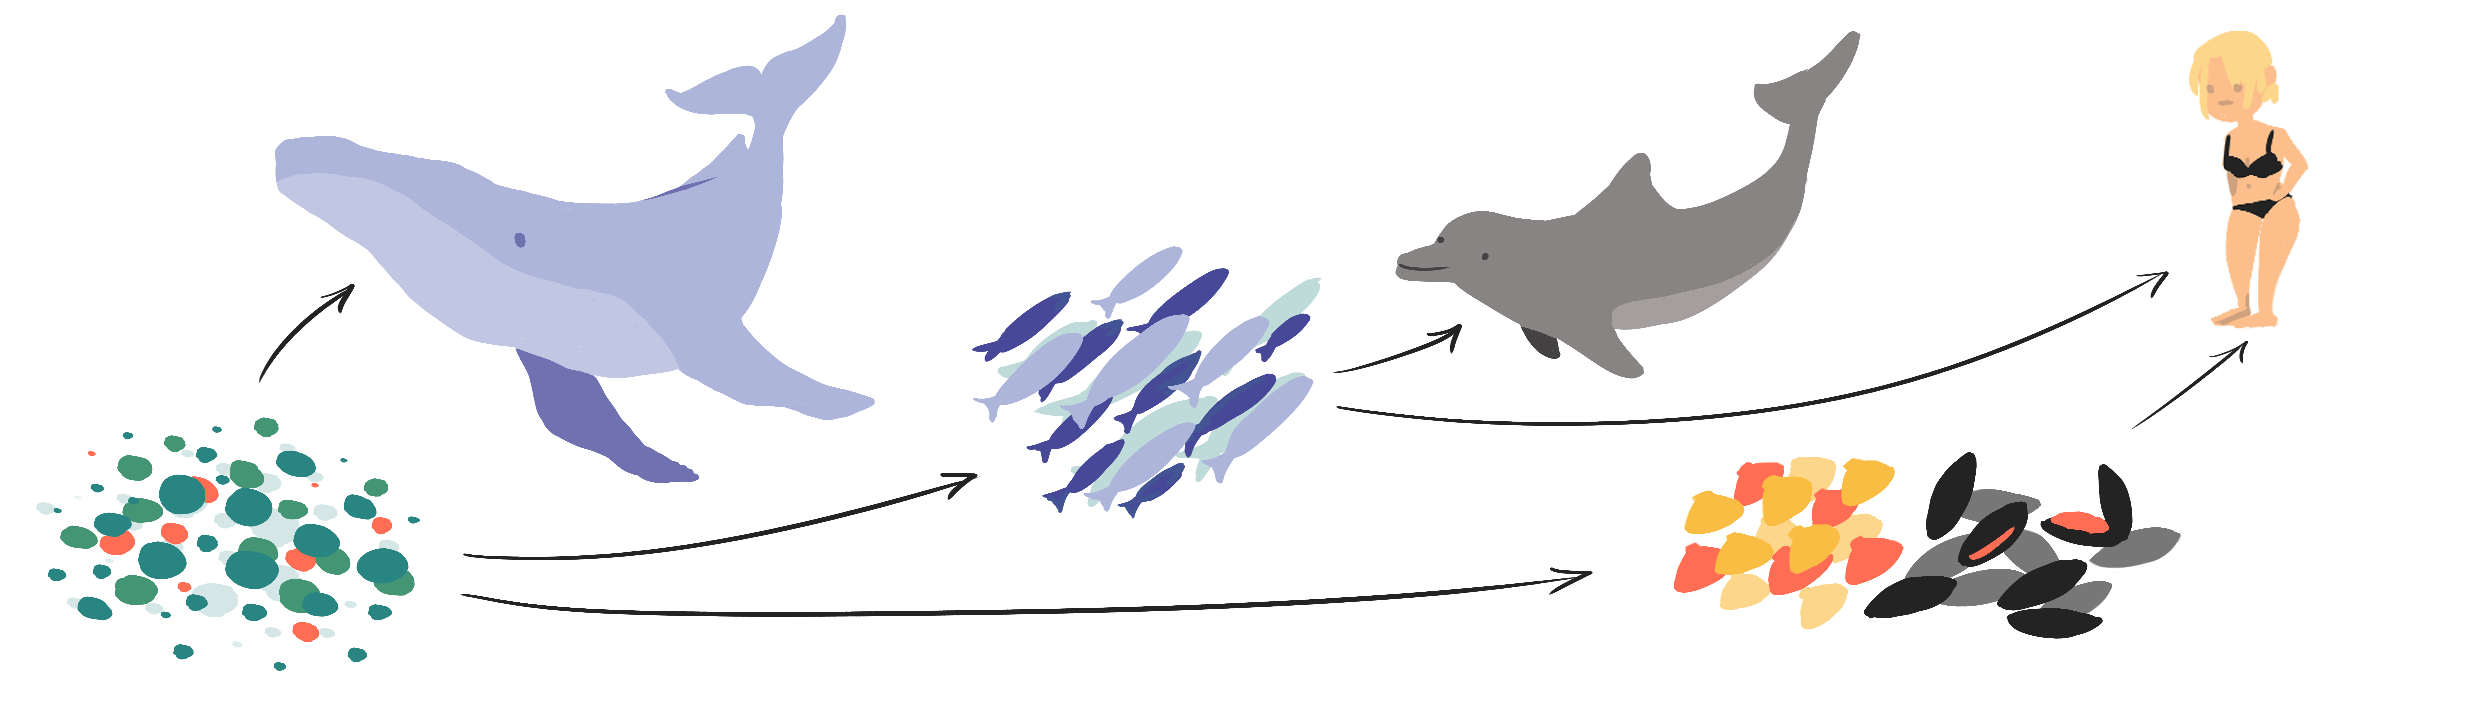
\includegraphics{food-chain}
    \caption[Marine toxins through the food chain]{Example of the advancement of marine toxins through the food chain by bioaccumulation}
    \labfig{food-chain}
\end{figure}

The most direct implication of this phenomenon lies in the seafood industry: when a harmful algal bloom occurs the mollusks that are being grown in the area become poisonous.
In order to prevent intoxications, the harvesting and selling has to be put on hold until the concentration of toxins in the water and in the seafood has gone down back to safe levels, with great economic losses for the fish market, the tourism industry and the restaurant business.\sidecite{hoagland02}

Specifically, STX is produced by phytoplanktons from the genera \genus{Alexandrium}, \genus{Gymnodinium} and \genus{Pyrodinium},\cite{gerssen10} as well as freshwater cyanobacteria bacteria including \genus{Anabaena} and \genus{Scytonema}.\cite{smith11,tebrineh10,}
When these species experience a bloom and free large quantities of STX into their ecosystem, families of bivalve organisms such as \genus{Mactridae}, \genus{Myacidae}, \genus{Mytilidae} and \genus{Veneridae} absorb it by filtration and accumulate it in their kidneys, feet and digestive glands\cite{oikawa05} until they reach hazardous concentrations.

Saxitoxin (STX), the protagonist of this introduction, is one of the substances that commonly become a threat when such blooms happen.
According to their chemical structure, marine toxins can be classified as domoic acid, saxitoxins, brevetoxins, okadaic acid, dinophysitoxins, pectenotoxins, yessotoxins, axaspiracids, spirolides and gymnodimines.\cite{gerssen10}\sidenote{STX, of course, belongs to the family of saxitoxins, but it's actually the head of a group with up to 57 different derivates.\cite{schantz75,bordner75,shimizu81}}

\begin{marginfigure}
    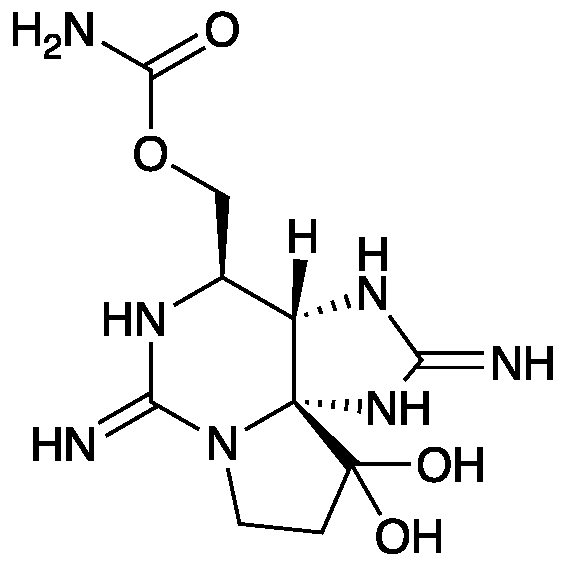
\includegraphics{stx-unlabeled}
    \caption[Structure of STX]{Structure of STX}
    \labfig{stx-unlabeled}
\end{marginfigure}

From a biological standpoint, STX and its family are responsible for a human syndrome known as paralytic shellfish poisoning (PSP).
PSP involves the binding of the toxin to the voltage gated sodium channels of the cells in the nervous systems, blocking the transmission of nervous impulses and effectively paralyzing the poisoned organism.
Specific symptoms of PSP in humans include numbness, headaches, dizziness, nausea, vomiting, diarrhea, weakness, temporal loss of vision, inability to breathe, and even death by respiratory paralysis.\cite{visciano16,gerssen10}
STX is such a potent neurotoxin, with an oral LD$_{50}$ for humans of only \SI{5.7}{\micro\gram\per\kilo\gram} of body weight,\cite{nguyen20} that is was considered and developed as a biochemical weapon by the United States in the past.\cite{stewart06}

For these reasons there exist health regulations, detection and quantification procedures that help identify algal blooms and regulate the seafood market.
Specifically, the standard procedure for the detection of STX is the mouse bioassay (MBA).
The MBA, which has a quantification limit of around \SI{370}{\micro\gram\per\kilo\gram}\sidecite{efsa09} consists in injecting an extract of a contaminated organism into a mouse.
The concentration of toxin in the contaminated sample can be estimated by measuring the time from injection to death.\cite{who84}
Apart from the bioethical issues that are inherently tied to this methods, it's also subject of another controversy.
The current regulatory limits in the European Union are of \SI{800}{\micro\gram\per\kilo\gram}.
However, by following acute reference dose (ARfD) criteria, we find out that the limits should be actually of \SI{75}{\micro\gram\per\kilo\gram}.\sidenote{Which results when taking the acute dose of \SI{0.5}{\micro\gram\per\kilo\gram} of body weight, and considering a \SI{60}{\kilo\gram} adult eating a reference portion of \SI{400}{\gram} of shellfish.}\cite{efsa09}
While its quantification limits are low enough to comply with the current EU regulations, they are insufficient when taking into account realistic health criteria.

There are newer alternative methods that don't rely on animal testing.
One of them is liquid chromatography with fluorescence detection and has a detection limit between \SI{10}{\micro\gram\per\kilo\gram} and \SI{80}{\micro\gram\per\kilo\gram}.\cite{eu17,aoac16}
This method, developed by AOAC Internacional,\sidenote{AOAC is a non-profit scientific association that publishes standarized chamical analysis methods.} is used as a co-official technique in the European union and has a good sensibility, but involves a series of derivatization steps and is time consuming.
Other common tests are enzime-linked inmunnosorbent assays\sidenote{More commonly known by their acronym ELISA}, which have a detection limit of about \SI{0.015}{\nano\gram\per\litre}.\cite{wharton17}
These are not reliable or sensible enough to be used for quantification, and are often relegated to screening purposes.

\begin{marginfigure}
    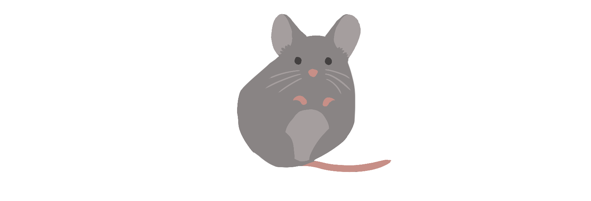
\includegraphics{mouse}
    %\caption[Structure of STX]{Structure of STX}
    \labfig{mouse}
\end{marginfigure}

The aim of this work in the context of the problem at hand, therefore, is to find realistic proposals for a better and more convenient method to identify and quantify STX.
To do this, the main focus of the research is put on spectroscopy.

\section{The work up until now}
\labsec{previous-work}

The author's involvement in finding appropriate spectroscopic techniques and environments for the detection of SXT dates back to previous work.
The efforts began with its computational characterization: modelling the STX, studying its acid-base behavior, assessing its conformational freedom in order to find its predominant structures...
After this preliminary treatment, several spectroscopic techniques were simulated and evaluated.

As a general approximation to vibrational spectroscopy, the vibrational normal modes were calculated and individually assessed in order to select a set of modes that, when present in a spectrum as peaks, could be used to unequivocally identify STX.
These modes could be visible in Infrared (IR) spectra, in Raman spectra, or in both.

IR spectroscopy was the first that was tested.
Vibrational modes are active in IR if by virtue of they symmetry they affect the dipole moment of a molecule.
The IR spectrum of the isolated STX was decently clear, and a good part of its characteristic vibrational modes were visible.
However, we had to take into account the fact that real life samples would consist mainly of seawater.
Water is very active in IR spectroscopy, with an ample signal between \SI{3500}{\per\cm} and \SI{4000}{\per\cm} due to stretchings, and a scissoring peak at \SI{1600}{\per\cm}.
These signals, with intensities proportional to the much higher quantities of water, would obscure those of the dilute STX, located near those same frequencies.
Extracting the STX from the water and redissolving it into a different solvent could be a way to fix this issue and make use of IR, but it would imply additional time and cost.

Water, however, has very weak signals in Raman.
Raman spectroscopy is able to detect vibrational modes that have an effect on the polarizability of a molecule.
This kind of spectroscopic technique relies on the effect of Raman scattering: a phenomenon in which the photons of a laser interact inelastically with molecular vibrations resulting in their energy being shifted up or down.
After generating Raman spectra for the STX, it was decided that the Raman active modes and their corresponding peaks would be sufficient to clearly identify the toxin.
There just remained the issue of the intensity: the effect behind Raman peaks has a very low probability, only one in every \num{1e7} photons that irradiate a molecule results in Raman scattering.
In a real experimental spectrum this translates into very low intensities that could easily get obscured by the noise from the signals of other molecules.
For this reason, the Raman spectroscopy had to be coupled with at least one amplification technique that could selectively amplify the signals related to STX.

The method chosen for this purpose was resonance Raman (RR).\sidecite{vidalvidal18-2}
While more about this effect and its fundamentals can be read in \refsec{rr-methods}, the practical simulation of RR can be summarized as \q{tuning the frequency of a laser so that the Raman scattering excitation coincides with an electronic transition}.
The problem with this approach was the following: while STX certainly benefits from resonance effects and Raman spectra with great amplifications can be generates, all of its electronic transitions are located below \SI{200}{\nano\metre}.
In a real life setting, it would be prohibitively expensive to use lasers of such small wavelengths: the most common lasers for RR range between \SI{244}{\nano\metre} and \SI{1064}{\nano\metre}, where the most common ones tend to be around the visible and near-infrared wavelengths.\cite{karlsson18,horiba}
Additionally, ultraviolet lasers tend carry more energy and could degrade the sample or result in autofluorescence effects that could interfere with the readings.
Since this work aims to propose feasible and practical ideas, we had to find a way to modify STX's natural range of absorption.
The answer lied close to the fundamentals of another Raman amplification technique: surface-enhanced Raman spectroscopy (SERS).
SERS is a variant of Raman that relies on the adsorption of a molecule onto a surface-like structure, usually composed of a metal.
While the Raman signal amplification was notable, the most interesting result that we found while studying SERS was the fact that adsorbing the STX to another molecule modified its electronic properties\sidenote{Resulting in what could be thought of as the shared electronic properties of a complex.} in such a way that its UV-vis absorption range was shifted towards larger wavelengths.

The system with which this effect was initially studied in previous work was a graphene sheet.
While the graphene-STX complex was successful in absorbing wavelengths longer than STX alone, it was found that the vibrations of the surface interfered with the identification of the molecule.

In this work, then, we intend to keep exploring that last idea: the binding of STX to another surface-like molecule with the aim of improving its electronic properties.
To continue the research along these lines would imply the selection of promising surface-like molecules, the characterization of the properties and spectroscopy of said molecules, and the study of their interactions with STX.


\section{The sunflower molecules: introduction and origin}

The search for effective and interesting SERS substrates ended up leading us to a novel class of molecules researched and presented in the year 2006 by Chernichenko and his team.\sidecite{chernichenko06}
The first representative of this family, nicknamed as \q{sulflower}, is the ocatathio[8]circulene.
This highly symmetric structure, which may be described as a form of carbon sulfide and as a belt of annulated thiophene cycles, is claimed to have great stability, high symmetry and unusual electronic properties.

From a synthetic point of view, sulflower also proved to be simple and straightforward to develop despite its complex appearance: start from tetrathiophene, sulphurize its free sites and acidificating to get polythiol, and remove the excess sulfur using vacuum pyrolysis.
%The tetrathiophene was
This process allowed the team to achieve yields of 56\% starting from commercially available reagents.

Interestingly, the team proposed that it could be possible to prepare materials with diverse electronic properties by using different types of heteroatoms and varying on the basic structure of the molecule.%
\begin{marginfigure}
    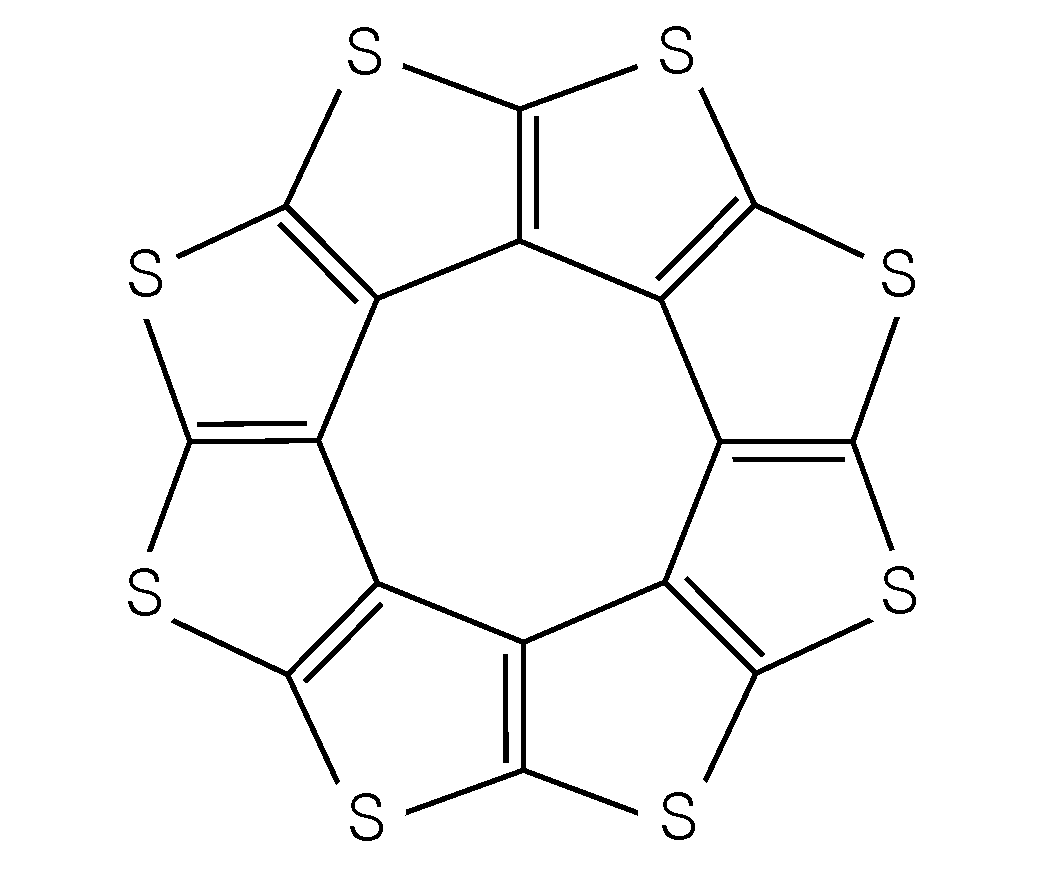
\includegraphics{sulflower-structure}
    \caption[Structure of sulflower]{Structure of sulflower}
    \labfig{sulflower-structure}
\end{marginfigure}%
Such a statement made apparent the potential of this family of molecules: stable, surface-like structures with varying degrees of symmetry and variable electronic behavior could act as suitable substrates for Raman amplification.
\refch{sunflowers} will be entirely dedicated to that premise: the study and characterization of sulflower and sulflower-like molecules, which from now on I will collectively refer to as \q{sunflowers} or simply \q{flowers}.
By designing, generating and studying our own family of sunflowers, we will be contributing to the characterization of a novel and interesting group of molecules, and we may be able to identify an ideal resonance Raman and SERS environment for STX.
Before that, however, a technical word on computational methods, calculation level, software and hardware.

\setchapterimage[2cm]{../images/header-methods.jpg}
%\setchapterpreamble[u]{\margintoc}
\chapter{Computational methods and specifications}
\labch{methods}

\section{Methods and techniques}

Throughout this work, many different computational methods and techniques were employed in order to carry out a diverse set of studies.
Some of them, the ones that are the most relevant to the flow of the work, are specifically explained and developed in detail in their own sections.
Others, however, are deemed to be more of a general character, already well known within the field, or unimportant for the understanding of the main ideas of this thesis.
This section is meant to serve as an overview of the methodology, specifications and theory behind the whole study, and also to provide explanations for that less special set of techniques.
This part may be skimmed and consulted at a later time, or even skipped entirely, as the rest of the work is presented in such a way that can be followed without deep knowledge of the subjects that are explained here.

\subsection{Calculation level}
All of the electronic structure calculations were performed using density functional theory (DFT) in the Kohn-Sham formulation.
Specifically, the functional of choice was Minnesota's M06-2X.\sidecite{truhlar08}
M06-2X is a highly parametrized hybrid meta-GGA functional that features a \SI{54}{\percent} of Hartree-Fock exchange.
It was chosen because it has been extensively trained to perform well in a variety of contexts that include thermochemistry, the study of non covalent interactions, and vibrational and electronic spectroscopy, appearing in numerous publications in the bibliography supporting its effectiveness.\cite{head16,vidalvidal17,vidalvidal17-2,vidalvidal18,sert14,eizig15,coccia17}
While the molecules discussed in the work are novel and have not been previously characterized, it's expected that their chemistry and their spectroscopic behavior aren't out of the ordinary.
Therefore, it should be possible to describe them properly and efficiently with such a functional.

As for the basis functions, the set of choice was Weigend and Ahlrichs' def2-SVP.\sidecite{ahlrichs05}
def2-SVP is of split valence and includes polarization functions, but is overall a fairly small set.
However, it was deemed sufficiently extense to obtain accurate geometry optimizations, and qualitatively good energies and spectra.

Considering the size of the systems of the study, the large amount of planned computations, the available computational resources, and the actual accuracy needs of the project, the M06-2X and def2-SVP calculation level was considered appropriate.

\subsection{Geometry optimization}
The optimization of the geometry of a molecule is a crucial part of any computational modeling.
At its core, it's a process where the geometry of a system gets iteratively modified (and its energy calculated at each step) with the aim of reaching a stationary point on its potential energy surface.
In the case of this work, these optimizations are always minimizations as we just look for energy minima.
In Gaussian09,\cite{gaussian09} our electronic structure computation software of choice, these calculations are carried out using the Berny algorithm in its GEDIIS\sidecite{li06} implementation.

\subsection{Magnetic shielding computation}
Nuclear magnetic resonance type calculations, namely the computation of the magnetic shielding in the nucleus-independent chemical shift study in \refsec{nics}, were carried out using the GIAO method.
GIAO stands for gauge-including atomic orbital.
It solves what is often referred to as \q{the gauge problem}, which can be defined as an error that arises when doing calculations with a magnetic perturbation while having the atomic orbital basis functions depend on position.\sidecite{magyarfalvi11}
Magnetic perturbations usually affect the atomic orbital set of a molecule as rotations.
Atomic orbitals located near to the axis of the rotation won't suffer from this error, as their basis sets should still be able to properly describe the perturbed wave function.
However, as the distance to the axis of rotation increases, the linear translation due to a rotation gets larger, and the description of the atomic orbitals gets progressively worse.
The GIAO method solves this problem by using sets of atomic basis functions that depend explicitly on the magnetic field.

GIAO calculations have been successful in describing the magnetic shielding of a variety of large nuclei in optimized and isolated large molecules.\sidecite{yuksek08} Therefore, it has been considered as an appropriate way of computing the absolute magnetic shieldings needed in this work.

\subsection{Electronic transition study}
\labsec{electronic-transition-study}
The prediction of ultraviolet-visible (UV-vis) spectra, a result of electronic transitions within a molecule, requires the computation of the energies of its electronically excited excited states.
As the electromagnetic waves responsible for such excitations have a time-dependent nature, in this work this is achieved through the application of time-dependent DFT.\sidecite{runge84,adamo13}

\subsection{Vibrational analysis}
Any given non linear molecule with $N$ atoms has 6 translational and rotational normal modes, and $3N-6$ vibrational ones.
Vibrational normal modes are orthogonal, that is, they're vibrational motions that are independent and don't cause movement to the other normal modes.

The frequencies of these modes are calculated through the following procedure.\sidecite{ochterski99}
All starts with a Hessian matrix that contains the second partial derivatives of the potential with respect to the displacement of the atoms.
This Hessian is mass weighted, its principal axes of inertia are determined, and it gets transformed into internal coordinates.
Through these operations, the rotational and translational modes get separated out and only the $3N-6$ vibrational modes remain.
Then, the transformed matrix is diagonalized.
The eigenvalues resulting from this diagonalization, $\lambda_i$, can be used to calculate the frequencies in wavenumbers ($\tilde{\nu_i}$) of each of the modes as described in \refeq{vibrational-frequencies}, where $i$ is a certain vibrational mode and $c$ is the speed of light.

\begin{equation}
    \labeq{vibrational-frequencies}
    \tilde{\nu_i} = \sqrt{\frac{\lambda_i}{4 \pi^2 c^2}}
\end{equation}

After this, the force constants and cartesian displacements for each of the modes can also be calculated.
The force constants $k_i$ can be obtained using \refeq{force-constants}, where $\mu_i$ is the reduced mass.

\begin{equation}
    \labeq{force-constants}
    k_i =  4 \pi^2 \tilde{\nu_i}^2 c^2 \mu_i
\end{equation}

The calculation of the cartesian displacements, on the other hand, can be summarized as \refeq{cartesian-displacements}.

\begin{equation}
    \labeq{cartesian-displacements}
    l_\textit{CART} = MDL
\end{equation}

In this equation, $M$ is a diagonal matrix defined by the masses of the atoms, $D$ is a transformation matrix that transforms from mass weighted cartesian coordinates to internal, and $L$ is a transformation matrix that holds the eigenvectors that result from the diagonalization of the internal coordinate Hessian.

\subsubsection{Normal mode calculation and decomposition}
\labsec{intmodes-methods}
By translating the cartesian displacements that result from the frequency calculations into redundant internal coordinates, it's possible to identify which of the atoms of the molecule or system are the most involved in a particular vibrational mode.
Having the vibrations expressed in such a way is useful in automating the analysis of modes.
In this work, this is used to classify the vibrational modes of a dimer.
Each individual vibration within the mode is classified by whether it belongs to molecule A, to molecule B, or is a mixture of the two.
Thanks to this calculation, the modes can be filtered by their percentage of A, B or mixed vibrations.
This idea is further explored and applied in \refsec{heatmaps}.

\subsection{Raman spectroscopy}
Raman spectroscopy is a technique that allows for the detection of those vibrational normal modes that affect the polarizability of a molecule (i.e. the ease with which its electron cloud can be distorted).
This kind of vibrational transitions are tied to a physical phenomenon known as Raman or inelastic scattering.
For an inelastic scattering event to happen, a photon has to excite a molecule and get it to a virtual energy state before being emitted.
After this, the photon has either a lower or a higher energy, and the molecule ends up in a different vibrational or rotational state due to the energy exchange between them.

Computationally, the intensity of a Raman active mode $i$ can be derived from its scattering factor $S_i$, which in turn it can be obtained from its polarizability tensor following \refeq{raman-activity}.
$Q_i$ represents the displacements of the vibrational mode, $\alpha$ is the isotropic polarizability, and $\gamma$ is the anisotropic one.

\begin{equation}
    \labeq{raman-activity}
    S_i = 45\left( \dv{\alpha}{Q_i} \right)^2 + 7\left( \dv{\gamma}{Q_i} \right)^2
\end{equation}

\subsubsection{Resonance Raman}
\labsec{rr-methods}
The regular Raman effect is usually very weak, as the probability of Raman scattering occurring is extremely low.\sidenote{Only about 1 in every \num{1e7} photons results in inelastic scattering}

\begin{marginfigure}
    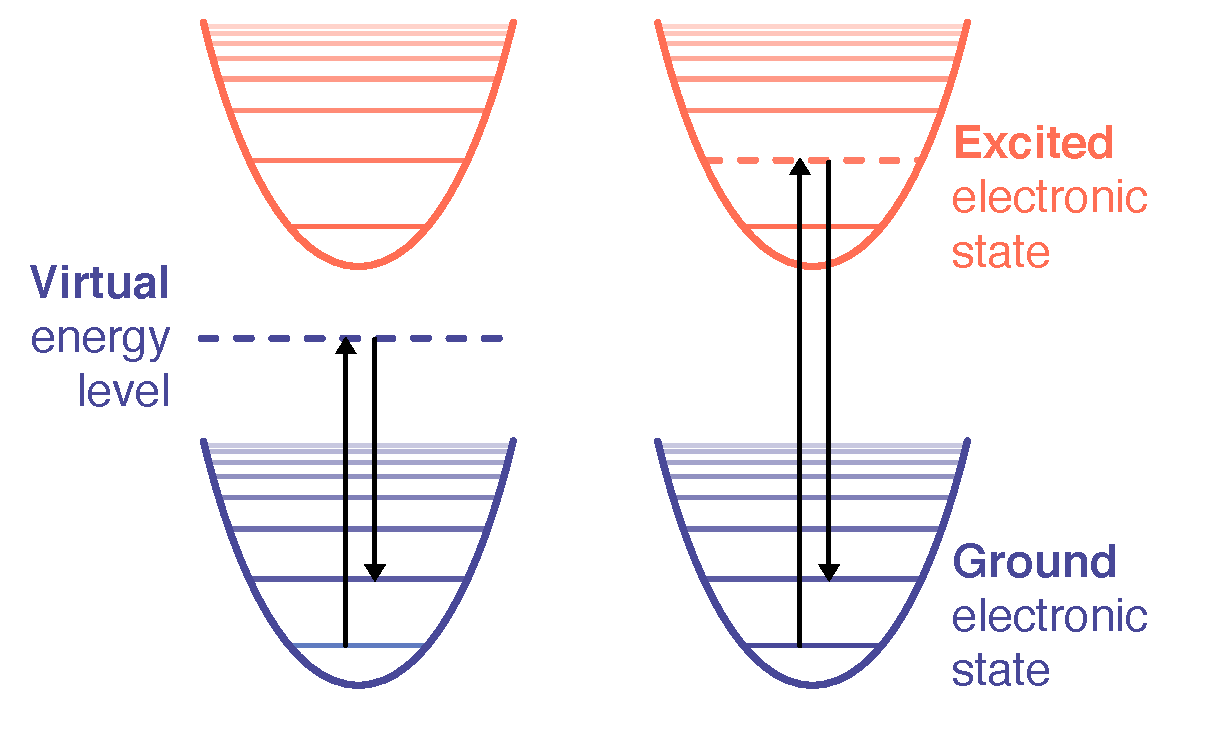
\includegraphics{raman-rr-comparison}
    \caption[Standard and resonance Raman excitations]{Standard and resonance Raman excitations}
    \labfig{raman-rr-comparison}
\end{marginfigure}

Resonance Raman (RR) spectroscopy is a variation of Raman in which the intensities are greatly amplified.
This technique relies in the usage of a carefully selected laser wavelength to perform the measurement: if it's close enough to an electronic transition, the scattering effect, and therefore the intensity of the measured Raman peaks, can increase by several orders of magnitude.
In regular Raman scattering, the energy that the molecule absorbs from the photon just makes it reach a virtual energy level before returning to a different rotational or vibrational state.
By using photons that have the same energy as electronic transitions, however, the molecule reaches a real excited electronic state as shown in \reffig{raman-rr-comparison}.
This excited state has a different geometry, and that affects the polarizability of the molecule and increases the magnitude of the subsequent Raman signal.\sidecite{hirakawa75}

These dynamic changes in the polarizability due to the electromagnetic radiation have to be taken into account in the calculation of the Raman intensities, and in Gaussian09 this is achieved through the introduction of perturbations by applying couple-perturbed DFT.

\subsubsection{Surface-enhanced Raman spectroscopy and surface interactions}
Surface-enhance Raman spectroscopy (SERS) is a variation of Raman spectroscopy that explores the large enhancements in intensity that the Raman signals of a molecule may experience when interacting with a surface.
While such effect was originally observed in roughened silver and is usually studied using metal surfaces and clusters, it has also been found in non-metal nanostructures and surface-like molecules.\sidenote{Which will be referred to as \q{SERS substrates} in general.}
The nature of this effect has been related to resonance.
Specifically, it's been said that it draws upon three different kinds: surface plasmon resonance, charge-transfer resonance, and molecular resonance.\sidecite{lombardi08}
The first of these effects, surface plasmon resonance, is defined as the coherence of the oscillation of the conduction electrons of the substrate\marginnote{Such as the free flowing electrons in a metal cluster, or the electron cloud of a large conjugated covalent system such as graphene} with an external exciting electromagnetic radiation.
Charge-transfer resonance may be present when there is a significant transfer of electron density between the substrate and the molecule.
Finally, molecular resonance may appear too as a property almost exclusive to the molecule, but can still have a significant contribution to the total effect.

The main focus of this work, however, is resonance Raman.
The adsorption of the molecule to a substrate makes it benefit from SERS effects, but it shares importance with its other purpose: shifting the UV-vis absorption range.
Adhering a molecule that absorbs short wavelengths to a substrate that absorbs long ones may result in a complex that has a range of absorption that's higher than that of the molecule alone.
Since real-life laser devices for Raman spectroscopy can get rare, expensive and energetic to the point of being destructive as the wavelength gets shorter, it's desired to achieve such effects.
For these reasons, while SERS is an interesting technique that certainly plays a part in the results achieved in this work, we don't delve too deep into the explanation of its nature.

\subsection{Spectra envelope calculation}
\labsec{spectra-envelope-calculation}

\begin{margintable}
    \centering
    \caption[Raman activity of STX]{Raman activity for each vibrational mode of STX in arbitrary units}
    \begin{tabular}{@{}c
                       S[table-format=1.4]
                       S[table-format=1.4]@{}}
        \toprule
        {Mode} & {$\tilde{\nu}$ (\si{\per\cm})} & {Ram. act.} \\
        \midrule
        1 & 0.0917 & 0.0236 \\
        2 & 0.9542 & 1.9687 \\
        3 & 0.8552 & 1.2691 \\
        4 & 1.7897 & 3.3270 \\
        \multicolumn{3}{c}{{\ldots}}
    \end{tabular}
    \labtab{oscillator-strengths}
\end{margintable}

This work deals with two types of spectra: electronic and vibrational.
Computational chemistry software is able to predict spectroscopic values such as electronic transition energies, vibrational mode wave numbers, Raman activities and oscillator strengths.
However, to get from those numbers to the familiar bands and peaks that are characteristic of experimental spectra, a few extra steps are involved.
This additional representation procedure will be exemplified by plotting both kinds of spectra for the saxitoxin (STX) molecule.

We start from the list of vibrational normal modes that results from a Raman calculation.
Then, their vibrational frequencies in the form of wave numbers as well as their corresponding Raman activity values are extracted using a custom script.
Plotting these values directly as vertical lines along the wave number range results in \reffig{without-envelope}.

\begin{figure}
    \centering
    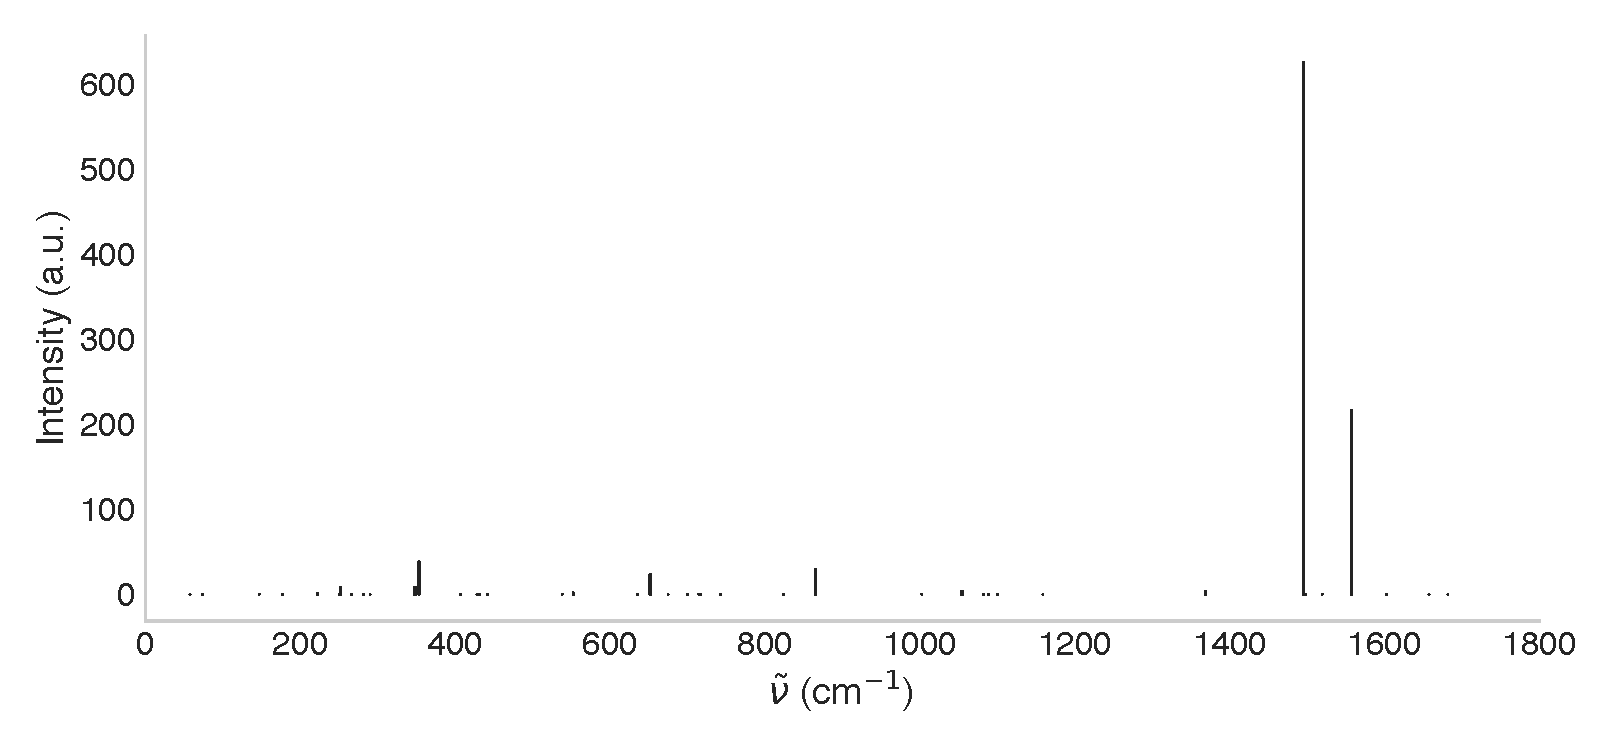
\includegraphics{without-envelope}
    \caption[Raman spectrum as simple peaks]{Raman spectrum of STX using a simple peak representation}
    \labfig{without-envelope}
\end{figure}

While such a graph could still be useful to display and compare the intensities of the vibrational modes, it could be harder to compare to real experimental spectra.
In order to make our theoretical spectra look more realistic, then, an envelope line is added.
This is done by replacing each of the simple vertical lines by Gaussian functions.
These functions are designed so that they are as tall as the intensity of the peak that they're representing.
They are evaluated at the full range of frequencies, and linearly combined forming a continuous curve that smoothly wraps all of the peaks.

In the case of Raman spectra, the value of each of the Gaussians at a certain wave number value is calculated following \refeq{raman-envelope}.

\begin{equation}
    \labeq{raman-envelope}
    I_i (\tilde{\nu}) = I_i^\textit{max}e^{-\left(\frac{\tilde{\nu} - \tilde{\nu}_i}{\sigma}\right)^2}
\end{equation}

The value of $\sigma$, which is the full width at half maximum of each curve, is set arbitrarily at \SI{4}{\per\cm}.
The same STX Raman spectrum, plotted after computing this set of equations, is displayed in \reffig{with-envelope}.

\begin{figure}
    \centering
    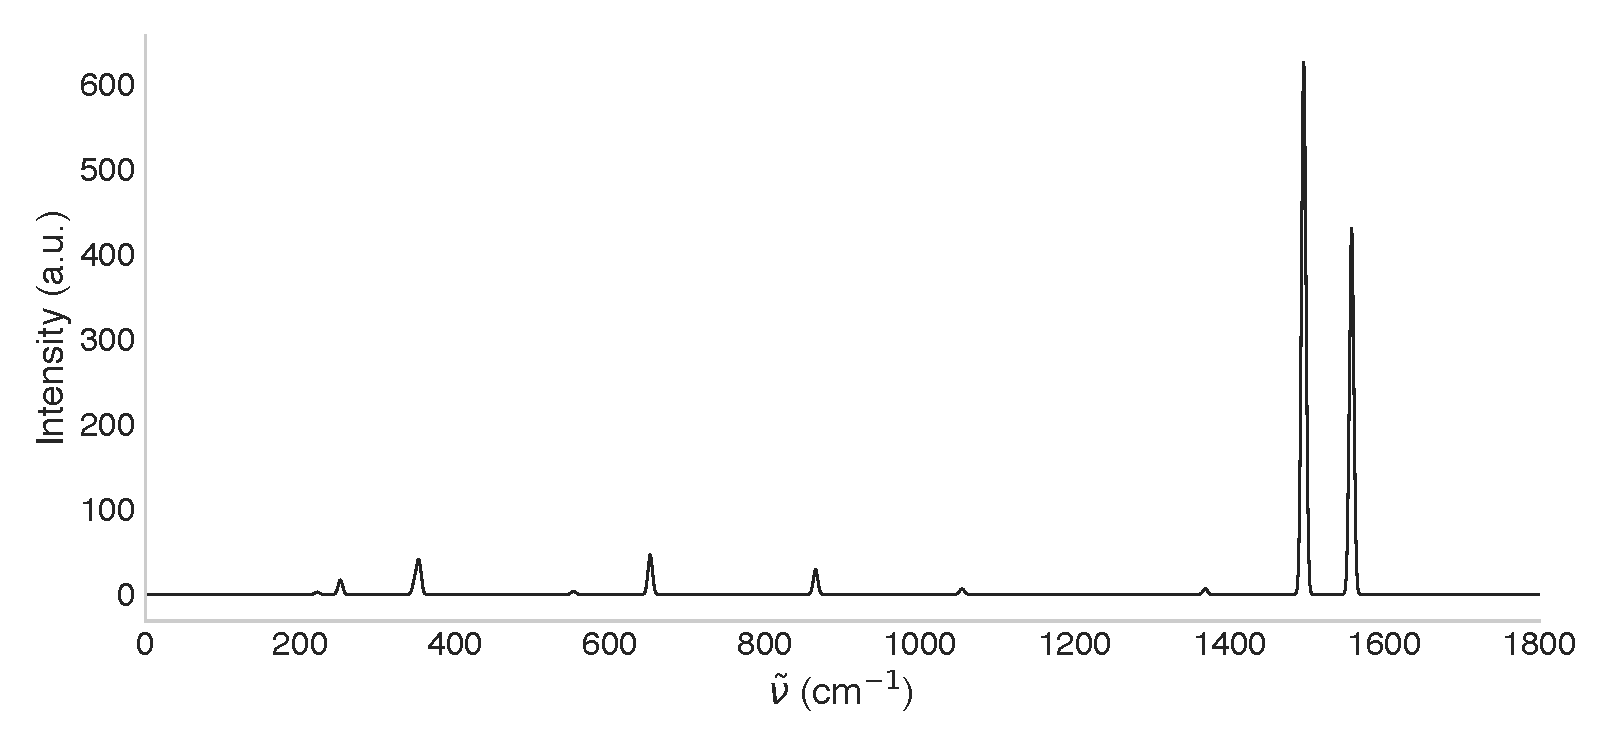
\includegraphics{with-envelope}
    \caption[Raman spectrum with Gaussian envelope]{Raman spectrum of STX using an envelope of Gaussian functions}
    \labfig{with-envelope}
\end{figure}

As for the electronic spectra, the procedure is quite similar.
In this case, the values to be plotted are the energies of the electronic transitions in the form of wavelengths, as well as their corresponding oscillator strengths.
Similarly to before, an envelope curve is created by calculating as many Gaussian functions as there are transitions, but with a slightly different formula as displayed in \refeq{uv-envelope}.

\begin{equation}
    \labeq{uv-envelope}
    \varepsilon_i (\lambda)) = \num{1.306297e8} \frac{f_i}{\sigma} e^{-\left(\frac{1/\lambda - 1/\lambda_i}{\sigma}\right)^2}
\end{equation}

Here, $\lambda_i$ and $f_i$ are the wavelength and oscillator strength of each transition. The constant before the exponential\marginnote{
\begin{equation}
    \labeq{uv-constant}
    \frac{\sqrt{\pi} e^2 N}{1000 \ln(10) c^2 m_e} = \num{1.306297e8}
\end{equation}
Where $e$ and $m_e$ are the charge and mass of the electron, $N$ is Avogadro's number, and $c$ is the speed of light
} (see \refeq{uv-constant}) is a conversion factor that is added in order to achieve the right units for the intensity $\varepsilon$, which should be \si{\litre\per\mole\per\cm}.
A value of \SI{0.4}{\eV} was chosen for $\sigma$.
For the case of STX, the spectrum that results from combining the Gaussian band shapes for the 50 most intense electronic transitions is shown in \reffig{uv-envelope}

\begin{figure}
    \centering
    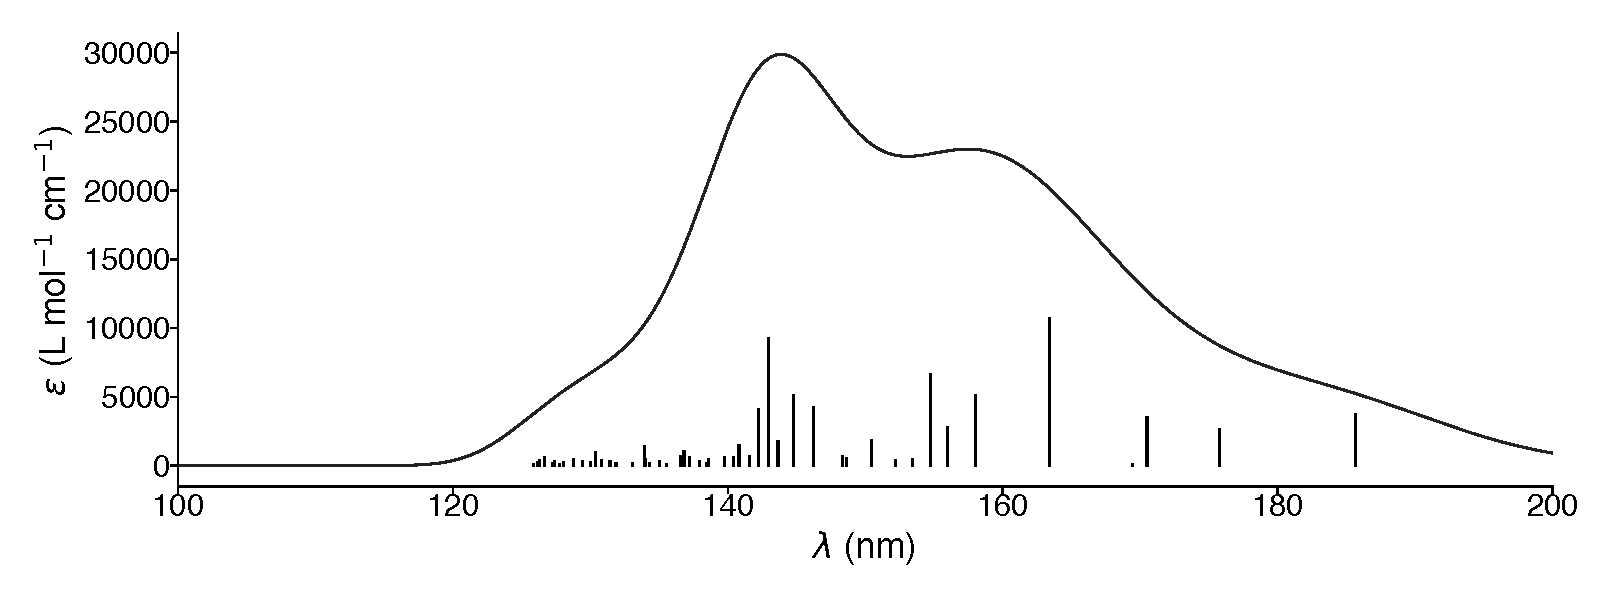
\includegraphics{uv-envelope}
    \caption[Electronic spectrum with Gaussian envelopes]{Electronic spectrum of STX using an envelope of Gaussian functions}
    \labfig{uv-envelope}
\end{figure}


\section{Software}

The software used to perform all of the calculations is summarized in \reftab{computational-techinques}

\begin{table*}[h]
    \centering
    \caption[Overview of techniques, level and software]{Overview of the computational techniques, calculation level and software that were used in this work}
    \labtab{computational-techinques}
    \begin{tabular}{@{}llllll@{}}
        \toprule
        Calculation & Technique & Spec. & Functional & Basis set & Software \\
        \midrule
        Geometry optimization                   & DFT       & GEDIIS    & M06-2X & def2SVP & Gaussian09 \\
        Vibrational analysis                    & DFT       &           & M06-2X & def2SVP & Gaussian09 \\
        Raman activity                          & DFT       &           & M06-2X & def2SVP & Gaussian09 \\
        Resonance Raman activity                & DFT       & CPDFT     & M06-2X & def2SVP & Gaussian09 \\
        Electronic transition calculation       & TD-DFT    &           & M06-2X & def2SVP & Gaussian09 \\
        Magnetic shielding calculation          & DFT       & GIAO      & b3lyp  & 6-31G*  & Gaussian09 \\
        Surface generation                      &           &           & & & nics.py \\
        \bottomrule
    \end{tabular}
\end{table*}


\section{Hardware}
All of the electronic structure calculations were performed using either the Centro de Supercomputación de Galicia's (CESGA) infrastructures, or the propietary cluster of the S3 research group.

CESGA's supercomputer, FinisTerrae-II (FTII), is a Bull ATOS bullx machines that features \num{320} computation nodes, \num{7712} cores, \SI{44544}{\giga\byte} of RAM, and \SI{750000}{\giga\byte} of storage capacity.
All of the calculations carried out at FTII were performed in standard nodes, utilizing \num{12} cores at a time, and \SI{60}{\giga\byte} of RAM.
These nodes include each 2 Intel\textregistered Xeon\textregistered E5-2630 v3 \SI{2.50}{\giga\hertz} processors with \num{24} cores total, and \SI{128}{\giga\byte} of RAM.

S3's cluster is composed of nodes that feature \num{16} cores running on Intel\textregistered Xeon\textregistered E5-2630 v3 \SI{2.40}{\giga\hertz} processors, and \SI{64}{\giga\byte} of RAM.

Smaller calculations such as input file generation, output parsing, surface estimation, graph representation... were carried out in the author's personal computer.

\setchapterimage[2cm]{../images/header-sunflowers.png}
%\setchapterpreamble[u]{\margintoc}
\chapter{Characterization of the sunflower molecules}
\labch{sunflowers}

\section{Sunflower design}

\begin{marginfigure}
    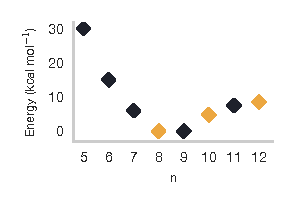
\includegraphics{sulflower-strain}
    \caption[Strain of thiophenic circulenes]{Strain of thiophenic circulenes with n rings}
    \labfig{sulflower-strain}
\end{marginfigure}

To start designing a family of molecules, first we must clearly state their defining pattern.
For this purpose, we adopt Chernichenko's own proposal: \q{a novel class of heterolytic circulenes}.
We start expanding the model by answering the question: are thiophene based circulenes with other than 8 rings stable enough to be worth considering?
The answer is in the original paper itself.
\reffig{sulflower-strain}, which was recreated to use our calculation level and adapt to the style of the document, shows that 8 ring structures are the most stable alongside 9 ring ones.
The details about this calculation are further explained in \refsec{study-of-stability}.
However, considering their low relative energies and the fact that they would have an even number of electrons even if (which would greatly simplify later calculations), 10 and 12 ring sunflowers were also chosen as part of the study.

Expanding upon this idea to allow for further heteroatom substitution, we ended up with the templates in \reffig{sunflower-skeletons}.
The possibilities were numerous, but we settled for S, Se, As and P substitutions on X$_1$ sites, and N substitutions in some cases in X$_2$ sites.
A full table detailing all of the structures that were generated and will comprise this study can be found in \reftab{sunflower-family}, as well as the short names or IDs that were given to each species based on its composition and number of petals for the sake of abbreviation.

\begin{figure*}
    \centering
    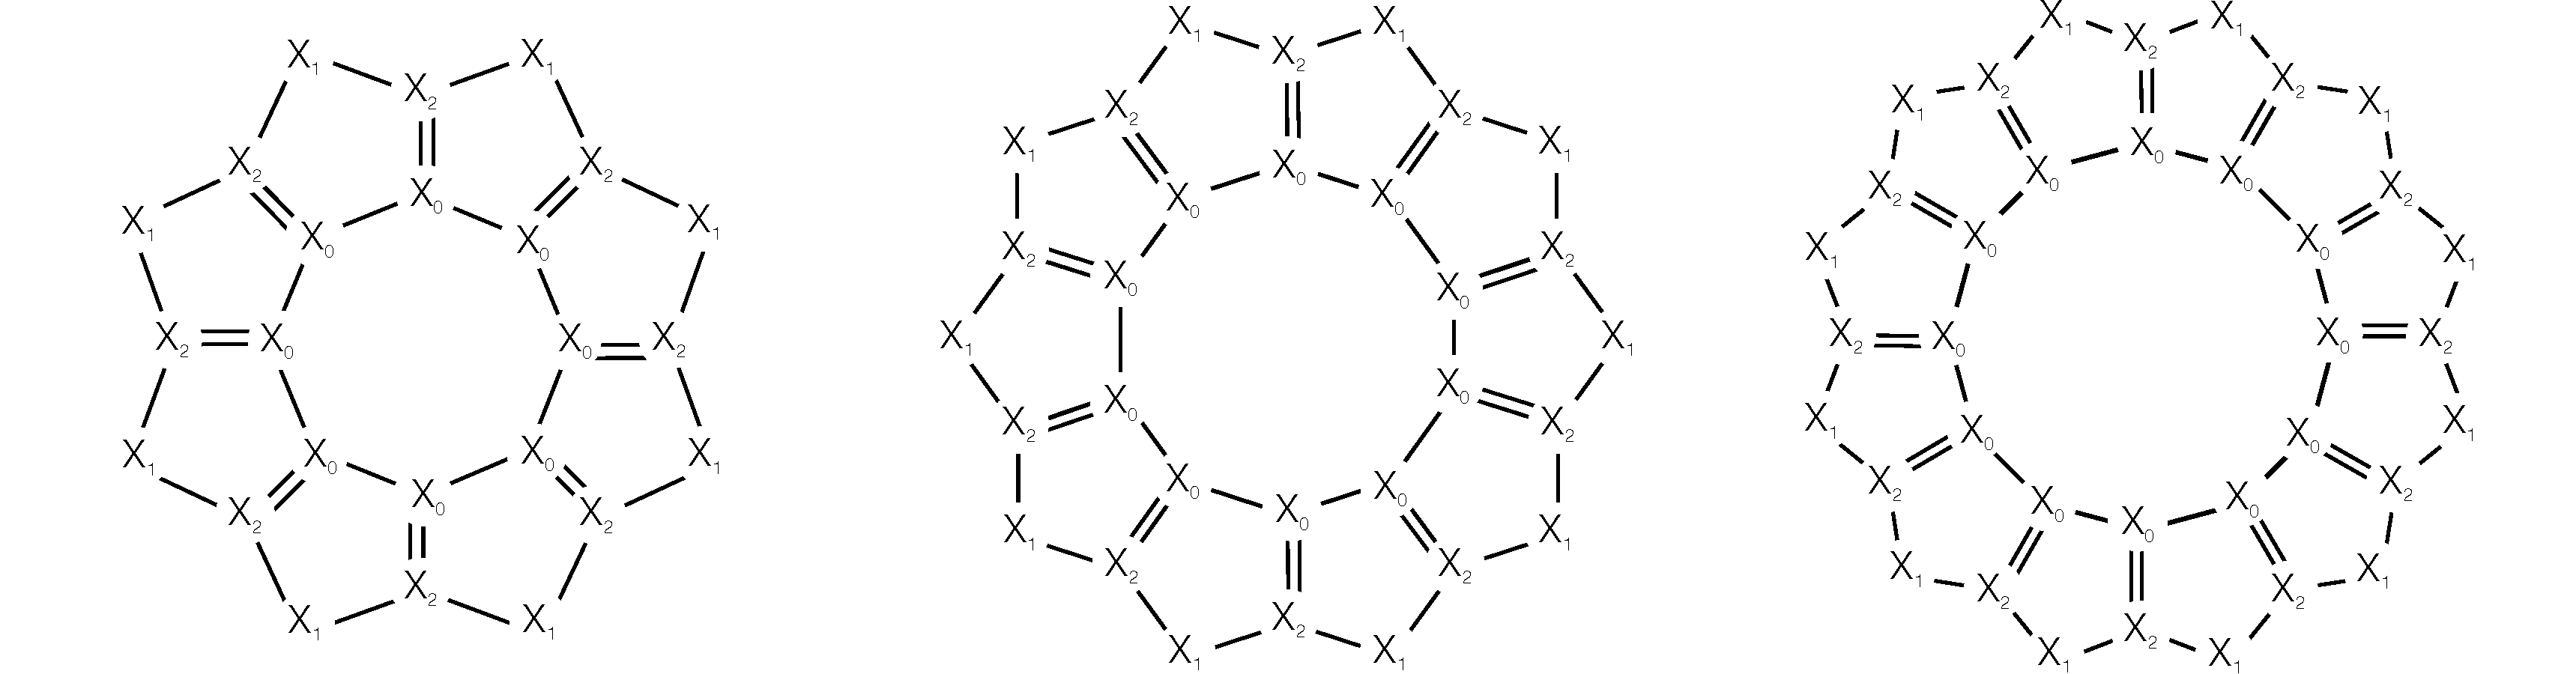
\includegraphics{sunflower-skeletons}
    \caption[General structures of the sunflower family]{From left to right, general structures of the 8, 10 and 12 ring sunflowers}
    \labfig{sunflower-skeletons}
\end{figure*}

\begin{table}
    \centering
    \caption[Sunflowers in this study]{Subset of the sunflower family that is going to be studied}
    \begin{tabular}{@{}cccrrr@{}}
        \toprule
        &&& \multicolumn{3}{c}{number of rings} \\
        X$_0$ & X$_1$ & X$_2$ & \multicolumn{1}{c}{8} & \multicolumn{1}{c}{10} & \multicolumn{1}{c}{12} \\
        \midrule
        C & S & C & S08 & S10 & S12 \\
        C & Se & C & Se08 & Se10 & Se12 \\
        C & As & C & As08 & As10 & As12 \\
        C & As & N & AsN08 & AsN10 & AsN12 \\
        C & P & C & P08 & P10 & P12 \\
        C & P & N & PN08 & PN10 & PN12 \\
        \bottomrule
    \end{tabular}
    \labtab{sunflower-family}
\end{table}


\section{Study of geometry}
\labsec{study-of-geometry}

Coordinate files for all of the designed sunflowers were created using the 3D molecule modeling program GaussView 6\sidecite{gv6}.
Then, they were optimized at the M06-2X/def2SVP calculation level.

\begin{figure}
    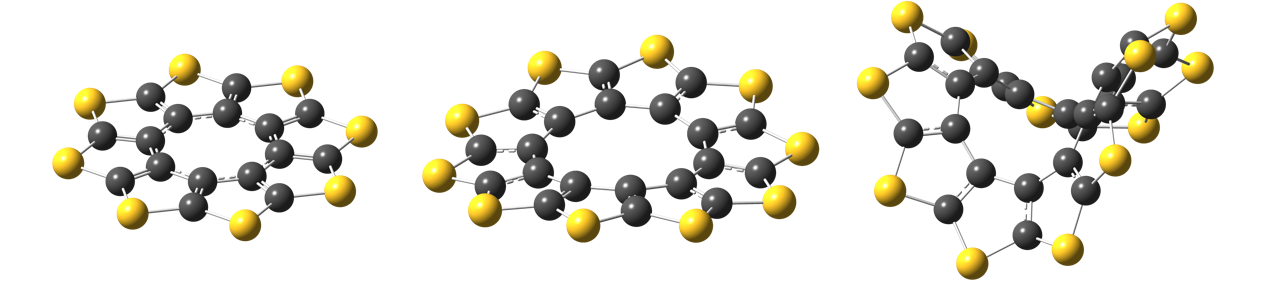
\includegraphics{sunflower-shapes}
    \caption[Shape of the sunflowers]{Shape of optimized S08, S10 and S12, from left to right (note the progressive increase in their deviation from planarity)}
    \labfig{sunflower-shapes}
\end{figure}

Using the output files for these calculations, all of the bond distances in all of the systems were extracted using Python.
Then, the bonds were grouped by type: inner (I, bonds between X$_0$ atoms, which were carbon in all cases), middle (M, between X$_0$ and X$_2$ atoms, which were either C-C or C-N bonds), and outer (O, between X$_2$ and X$_1$ atoms).
The mean and standard deviation of these groups were computed for all of the flowers and displayed in \reftab{bond-length-study}.%
\begin{marginfigure}
    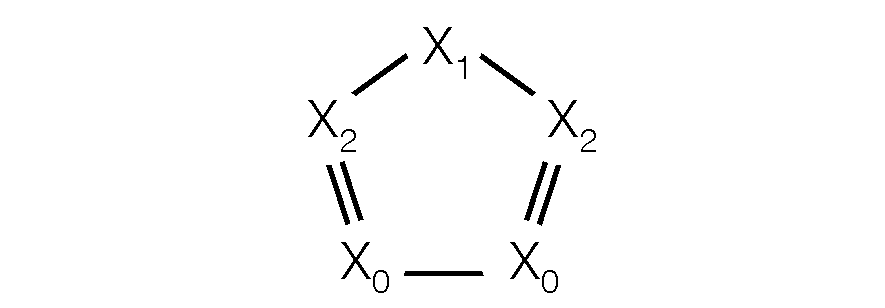
\includegraphics{pentagon-structure}
    \caption[Single petal structure template]{Single petal structure template (hydrogen is added to adjust for neutrality as needed)}
    \labfig{pentagon-structure}
\end{marginfigure}%
Additionally, pentagonal structures of the form displayed in \reffig{pentagon-structure} were modeled and optimized, and their bond length data was compared with the rest and also presented in \reftab{bond-length-study}.
These are used to compare the geometry of the flowers with that of single petals.

How is this information useful?
In the first place, it allows us to easily compare the average length of each bond type as the number of units increases.
More interestingly, it serves as a way to assess the nature of each bond group.
Take the inner C-C bonds.
In all cases, the average length lies between the usual values for single and double C-C bonds,\sidenote{\SI{1.54}{\angstrom} for single and \SI{1.34}{\angstrom} for double bonds\cite{chang12}} an information that immediately suggests us that the flowers might be conjugated systems with $\pi$ electron delocalization.
However, it could also be possible that there were equal amounts of single and double bonds, and that these apparently conjugated bond lengths were just a the result of a lousy statistical approximation.
That's why the $\sigma$ metric was also computed.
Groups with a relatively high $\sigma$ such as the I bonds of As08, As12, P08 and P12 are actually composed of longer and shorter bonds, and it's likely that their $\pi$ electrons aren't delocalized.
On the other hand, groups with small $\sigma$ values are more likely to correspond to conjugated systems, which may be stabilized by electron delocalization.
This concept of bond length equalization and conjugation may be tied to that of aromaticity, where equalized C-C bonds could be a sign of it, and uneven ones could indicate non aromaticity or antiaromaticity.\sidecite{zhongfang05} This topic will be covered in greater detail in \refsec{study-of-aromaticity}.

\begin{table}
    \centering
    \caption[Bond length study]{Bond length statistics for each studied species, units are \si{\angstrom}, and $\tilde{x}$ and $\sigma$ are the mean and the standard deviation}
    \begin{tabular}{@{}rlcccccc@{}}
        \toprule
        && \multicolumn{2}{c}{I (X$_0$-X$_0$)} & \multicolumn{2}{c}{M (X$_0$-X$_2$)} & \multicolumn{2}{c}{O (X$_1$-X$_2$)} \\
        && $\tilde{x}$ & $\sigma$ & $\tilde{x}$ & $\sigma$ & $\tilde{x}$ & $\sigma$ \\
        \midrule
        \multirow{4}{*}{S} & ring & 1.429 & - & 1.367 & 0.000 & 1.719 & 0.000 \\
        & 08 & 1.423 & 0.000 & 1.377 & 0.000 & 1.754 & 0.000 \\
        & 10 & 1.482 & 0.000 & 1.399 & 0.000 & 1.712 & 0.000 \\
        & 12 & 1.466 & 0.004 & 1.389 & 0.000 & 1.732 & 0.004 \\
        \\
        \multirow{4}{*}{Se} & ring & 1.434 & - & 1.363 & 0.000 & 1.857 & 0.000 \\
        & 08 & 1.454 & 0.000 & 1.385 & 0.000 & 1.865 & 0.000 \\
        & 10 & 1.478 & 0.003 & 1.389 & 0.000 & 1.861 & 0.004 \\
        & 12 & 1.466 & 0.007 & 1.381 & 0.000 & 1.877 & 0.005 \\
        \\
        \multirow{4}{*}{As} & ring & 1.468 & - & 1.354 & 0.000 & 1.918 & 0.000 \\
        & 08 & 1.434 & 0.050 & 1.448 & 0.000 & 1.859 & 0.008 \\
        & 10 & 1.436 & 0.000 & 1.454 & 0.001 & 1.856 & 0.001 \\
        & 12 & 1.435 & 0.042 & 1.446 & 0.002 & 1.867 & 0.007 \\
        \\
        \multirow{4}{*}{AsN} & ring & 1.495 & - & 1.283 & 0.000 & 1.854 & 0.000 \\
        & 08 & 1.434 & 0.000 & 1.361 & 0.000 & 1.858 & 0.000 \\
        & 10 & 1.450 & 0.001 & 1.364 & 0.001 & 1.856 & 0.004 \\
        & 12 & 1.440 & 0.004 & 1.357 & 0.001 & 1.873 & 0.006 \\
        \\
        \multirow{4}{*}{P} & ring & 1.467 & - & 1.359 & 0.000 & 1.794 & 0.001 \\
        & 08 & 1.410 & 0.048 & 1.445 & 0.000 & 1.764 & 0.006 \\
        & 10 & 1.431 & 0.000 & 1.471 & 0.000 & 1.736 & 0.000 \\
        & 12 & 1.429 & 0.045 & 1.462 & 0.002 & 1.747 & 0.005 \\
        \\
        \multirow{4}{*}{PN} & ring & 1.485 & - & 1.293 & 0.000 & 1.707 & 0.000 \\
        & 08 & 1.404 & 0.000 & 1.364 & 0.000 & 1.752 & 0.000 \\
        & 10 & 1.448 & 0.000 & 1.385 & 0.000 & 1.715 & 0.001 \\
        & 12 & 1.435 & 0.002 & 1.378 & 0.001 & 1.732 & 0.004 \\
        \bottomrule
    \end{tabular}
    \labtab{bond-length-study}
\end{table}


\section{Study of stability}
\labsec{study-of-stability}

Using the output files from the previous step, specifically those from the initial optimization, calculations related to the energies of the flowers were performed in order to assess their stabilities.

\subsection{Ring strain}
\labsec{ring-strain}
Ring strain may be defined as a kind of instability that arises when angles of the bonds in a cyclic molecule deviate from their optimal values, which they would be able to adopt if they weren't coiled in the shape of a ring.
The energy associated to this phenomenon can serve as a way to compare the stabilities of flowers with different numbers of petals, as it was done in the original paper and reproduced in \reffig{sulflower-strain}.
Its calculation relies on the design of an homodesmotic reaction.
What does this mean?
In a homodesmotic reaction, the number of atoms and the type of hybridations in the products are the same as in the reactants.
Our goal is to devise a chemical equation where the strained structure appears in only one of its sides and the rest of the chosen molecules don't present any strain effects.\sidecite{vidalvidal18}
If we manage to create such an equation, the reaction energy will correspond to the strain, as the rest of the components of the energy should nullify themselves between the two sides of the reaction.

In this case, apart from the sunflower structure B, the equations that were designed included molecules A and C, non-cyclic structures composed of 3 and 2 petals. \marginnote{
	\begin{equation}
        \labeq{homodesmotic-equation}
        E_\text{strain} = \frac{E_B + nE_C - nE_A}{n}
	\end{equation}
} By following this reaction, which is fully displayed in \reffig{homodesmotic}, the strain energy was calculated as shown in \refeq{homodesmotic-equation}.

\begin{figure}
    \centering
    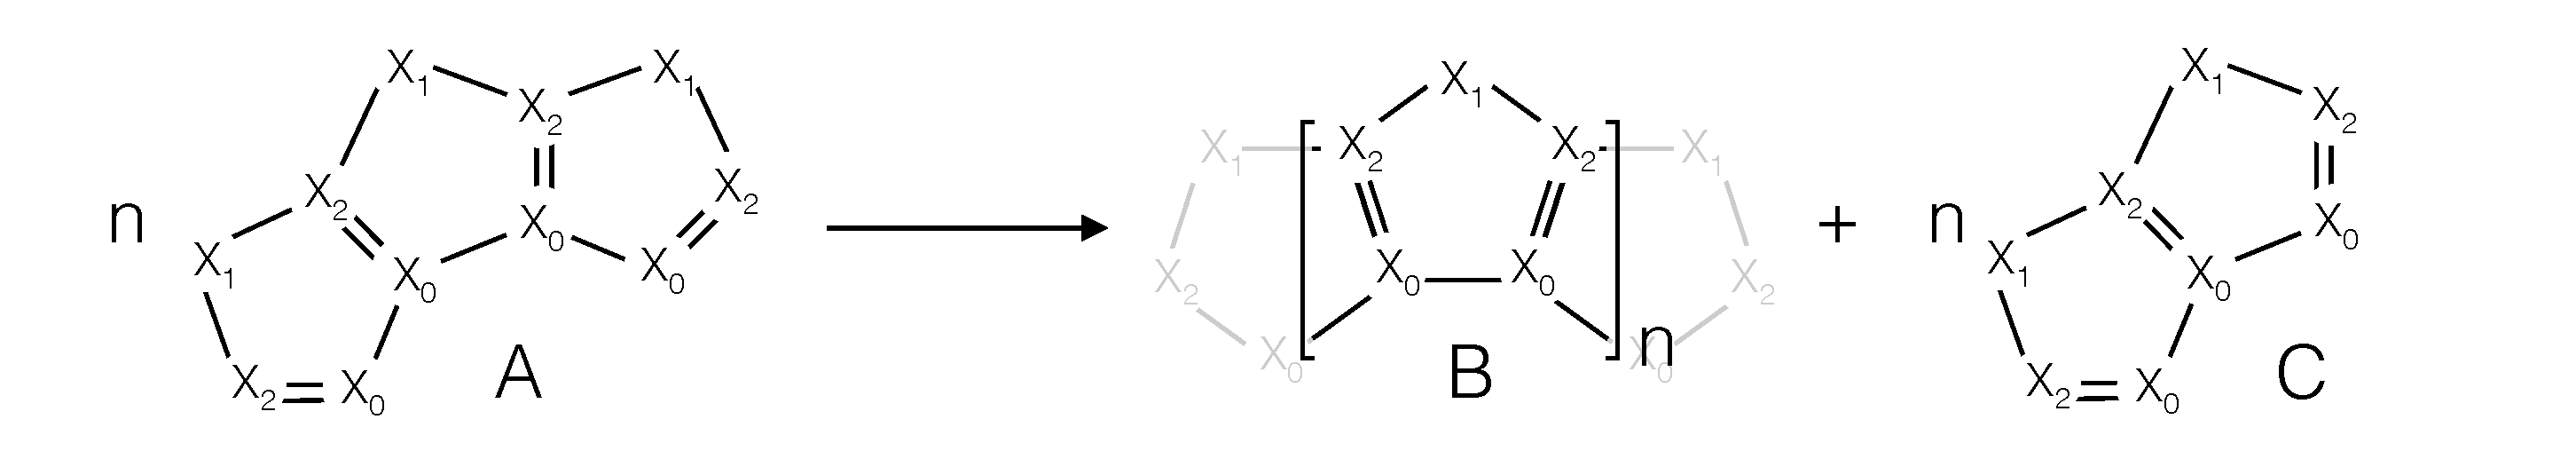
\includegraphics{homodesmotic}
    \caption[Homodesmotic reaction used to calculate strain energies]{Homodesmotic reaction used to calculate strain energies}
    \labfig{homodesmotic}
\end{figure}

This calculation, which is the one that was used to generate the previous sulflower stability curve \reffig{sulflower-strain}, was applied to all of the sunflowers of the study, and the resulting strain energies are presented in \reffig{sunflower-stability}.
As it can be seen, the strain energies always increase with the number of petals (as it's the case for the original sulflower series).
However, it may be noted that their increase follows slightly different tendencies.
Notable examples are the P family, where the 8 and 10 petal species have very similar strains; and the Se, As and AsN families, where the energies of the 10 and 12 petal structures are very close.
These energy values are an useful indication of the relative strains of the different species within a family, and an estimation of their
stabilities with respect to the original sulflower.
Nevertheless, it should be kept in mind that this calculation is an approximation, and that the values of the so called strain energy might be accounting for other effects such as conjugation stabilization or repulsion between the heteroatoms.

\begin{figure}
    \centering
    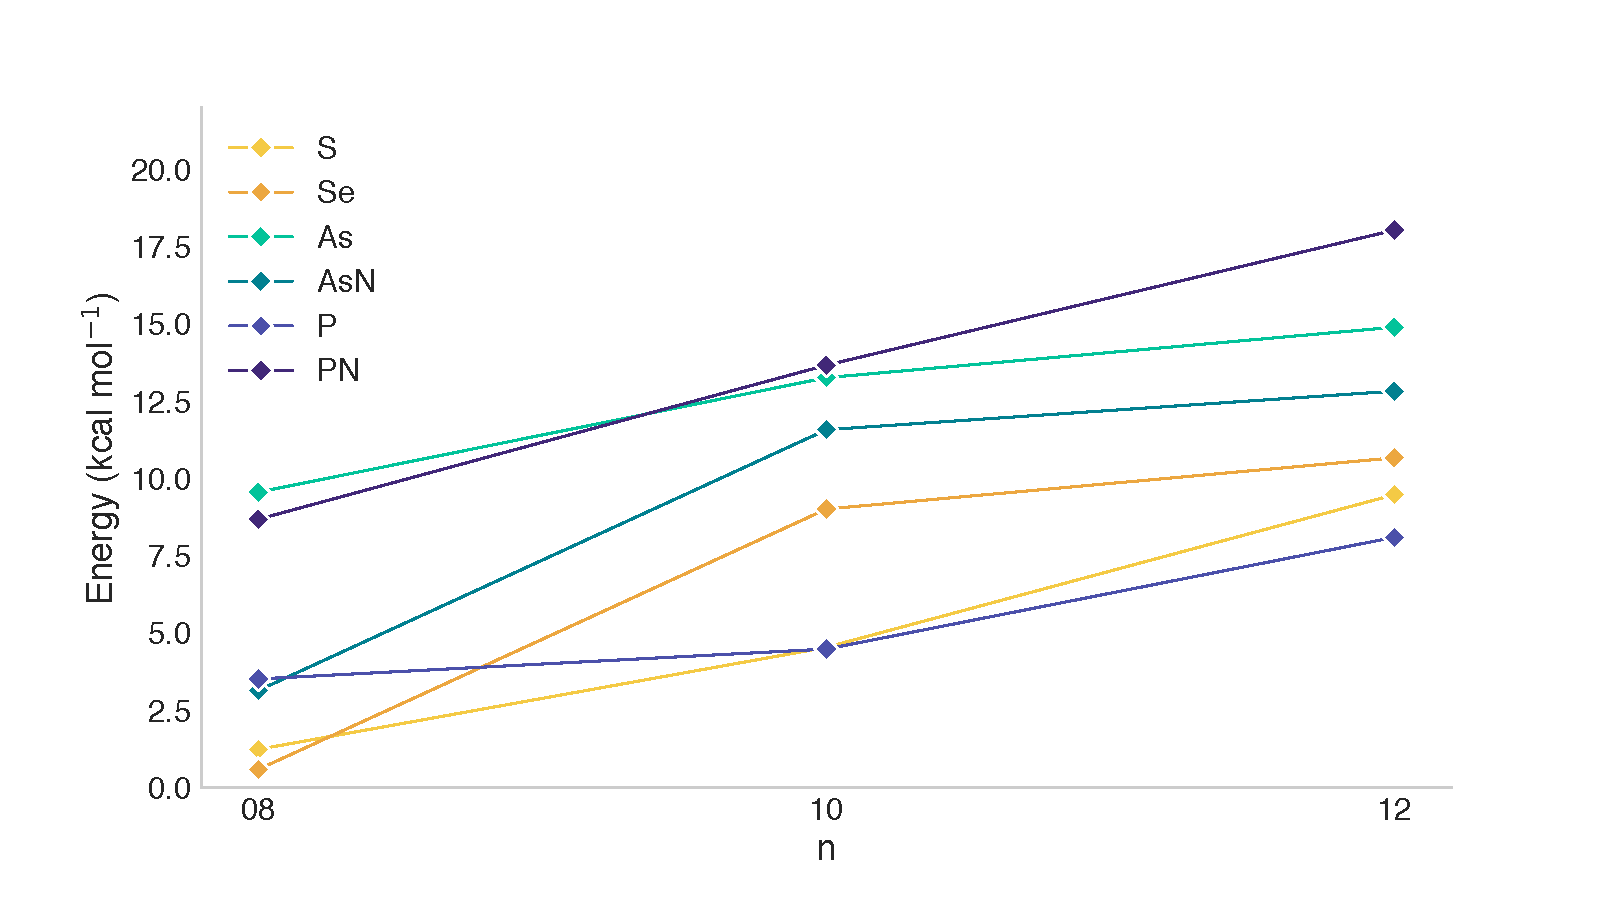
\includegraphics{sunflower-stability}
    \caption[Strain energies of sunflower groups]{Strain energies of all of the studied sunflower groups}
    \labfig{sunflower-stability}
\end{figure}


\section{Study of aromaticity}
\labsec{study-of-aromaticity}

Aromaticity is a property related to molecules that contain a ring or a chain of resonance bonds that increases their stability.
It’s typically found in flat ring structures, although the definition has been discussed and expanded since its initial association to benzene\cite{faraday1825} and there are other varieties such as annulenic, azulenic, inorganic, homoaromatic, three-dimensional, $\sigma$-electron, and even metallic electron aromaticity.\sidecite{zhongfang05}
Considering their ringed structure and possibly high conjugation, we wondered if the sunflowers could present any kind of aromatic tendencies.
Having already studied their degree of bond length equalization in \refsec{study-of-geometry}, we set out to assess their aromaticity from the point of view of their magnetic properties.

\subsection{Nucleus-independent chemical shift}
\labsec{nics}
Since its introduction in 1996 by Schleyer et al.\sidecite{schleyer96}, Nucleus-independent chemical shift (NICS) has become the most popular and widely used technique to estimate aromaticity in a quantitative way.
It's based on the study of electronic ring currents.
As the electrons in the possibly-aromatic systems have a certain degree of free circulation, an external magnetic field perpendicular to the main plane of the system is able to induce a ring current.
Said ring currents generate their own magnetic field, which can weaken or strengthen the effect of the external field, resulting in decreased or increased NMR chemical shifts.
Aromatic systems will experience shielding on the inside of the ring and deshielding on the outside.
Antiaromatic systems will experience the opposite.

\begin{margintable}
    \centering
    \caption[Popular NICS variants]{Popular NICS variants depending on the location of the molecule in which the magnetic shielding is calculated}
    \begin{tabular}{@{}ll@{}}
        \toprule
        Name & Measurement \\
        \midrule
        NICS(0) & At the center of the ring \\
        NICS(1) & \SI{1}{\angstrom} above the center \\
        NICS$_\textit{zz}$ & Out-of-plane \\
    \end{tabular}
    \labtab{nics-variants}
\end{margintable}

\subsubsection{The basic application of NICS}
NICS is usually applied to single rings, and quantified by computing the absolute magnetic shielding at key locations.
This key location is usually one of the following: the center of the ring (calculated as the non-weighted mean of the positions of the heavy atoms), several points along a central axis perpendicular to the plane of the ring (calculated trivially in planar rings as the plane that passes through any three ring atoms), at several points on a grid perpendicular to the plane of the ring, or as three dimensional isosurfaces using dense grids.
Considering this location criterion, some of the most applied variants of NICS have been summarized in \reftab{nics-variants}.

\subsubsection{A custom solution for non-planar molecules}

\begin{marginfigure}
    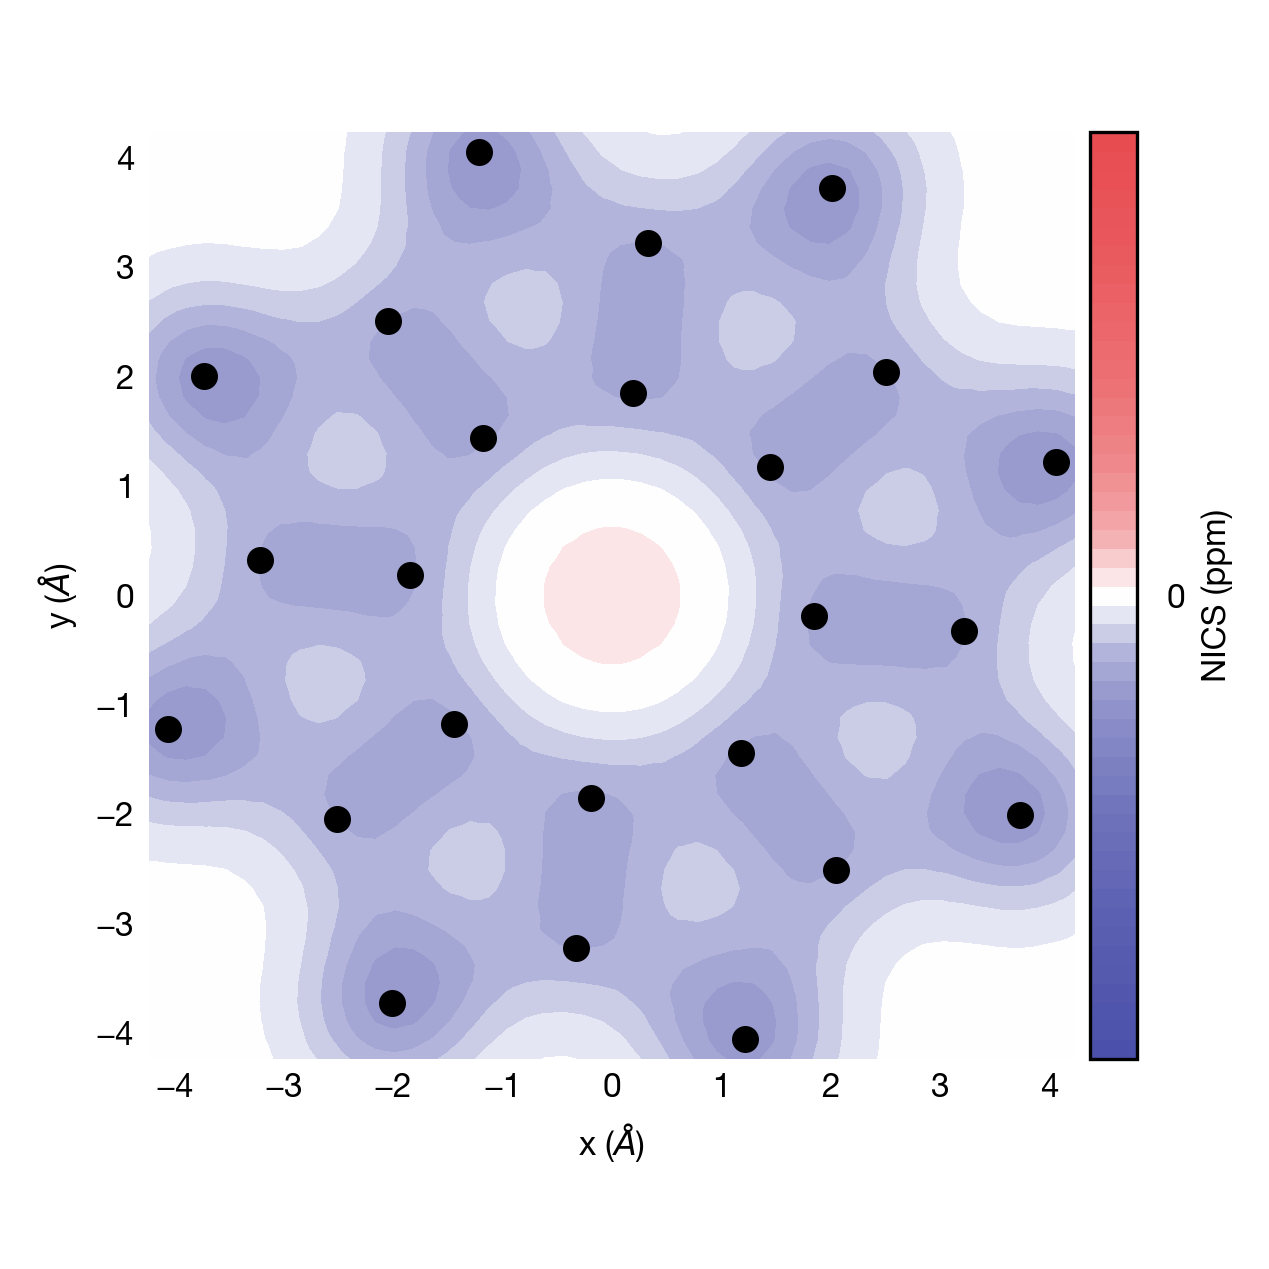
\includegraphics{s08-2d}
    \caption[NICS applied to sulflower]{Custom NICS technique applied to the original 8 petal sulflower molecule as a sample of the legacy approach}
    \labfig{s08-2d}
\end{marginfigure}

A seen in \reffig{sunflower-shapes} in \refsec{study-of-geometry}, 8 petal sunflowers are perfectly planar.
In previous studies, NICS calculations on flat grids parallel to their planes were applied with success.
All of the points of the grid were equidistant to the plane of the molecule to be able to properly compare their values (the magnitude of the magnetic shielding decreases the farther away from the molecule that it is measured).
The positive values of the magnetic shielding were plotted in red and the negative ones in blue, which overlaid over the atoms of the flower, resulted in graphs like \reffig{s08-2d}.
However, 10 and 12 petal sunflowers have bended and warped shapes, and the \q{general plane} of the molecule is no longer a plane.
In order to translate the old method, a new approach was developed and applied.
The idea of extending a grid of points over the surface of the system and plotting it as a 2D projection is maintained, but what is exactly the surface of a non planar molecule, and how can it be generalized for non planar molecules?

Defining the concept of \q{general surface} for a warped ring is a tricky task, but we've set on the following description: a 3D surface that is equidistant to all of the heavy atoms of a molecule and to all of the middle points of their bonds, and that follows a smooth and intuitive tendency in the places where are neither atoms nor bonds. A general surface could be loosely thought of as a blanket that was being draped over a physical molecular model of the system, sitting on the places where there are balls and sticks, and covering the empty spaces smoothly without caving in.

To mathematically model such an idea, several approaches were evaluated and tested,\sidenote{Such as using interpolation algorithms to calculate the grid points in the empty spaces, or generating compound surfaces by tiling all of the possible planes based on groups of three atoms.} but in the end, the method was based on linearly combining a set of simple 3D cartesian functions.

This idea was born while thinking about the curvature of the largest sunflowers.
\q{This Se10 molecule looks like it has the shape of a saddle.\sidenote{The equation of a basic saddle is essentially $z=x^2-y^2$.} What if we could find the precise parameters for a saddle that adjusted to the shape of this molecule?}
This concept was expanded to include a wider variety of molecules and shapes: there's a limit to the angles and deformations that a ring in a molecule can display... so therefore, it should be possible to get a decent approximation to any molecular surfaces by combining and fine tuning a selection of common 3D shapes in the form of functions.
The remaining question is... how can we find which 3D functions should be used, and what coefficients should be assigned to them?
The functions were picked out by hand, and will later be enumerated and justified.
The coefficients, however, had to be calculated somehow.
Our solution, which will be fully explained hereunder, relies upon the core concepts of statistical learning.

\begin{margintable}
    \centering
    \caption[xyz coordinates]{xyz coordinates of the atoms of Se10}
    \begin{tabular}{@{}S[table-format=1.4]
                       S[table-format=1.4]
                       S[table-format=1.4]@{}}
        \toprule
        $x$ & $y$ & $z$ \\
        \midrule
        0.9154 & 0.0917 & 0.0236 \\
        -0.0971 & 0.9542 & 1.9687 \\
        1.0978 & 0.8552 & 1.2691 \\
        1.8126 & 1.7897 & 3.3270 \\
        \multicolumn{3}{c}{{\ldots}}
    \end{tabular}
    \labtab{xyz}
\end{margintable}

First off, we start with just the coordinate file of the optimized structure of the studied molecule.
We will use Se10 as an example.
This file should contain the position of each of the atoms in the 3D cartesian space relative to the origin of coordinates (i.e., an xyz file).
In order to stabilize the calculations and apply the method properly, the molecule has to undergo two transformations: it has to be translated so that its center coincides with the origin of coordinates $(0,0,0)$; and it has to be rotated so that its main axis aligns with $z$, or $(0,0,1)$.

The first one is trivial, the centroid of the ring is calculated as the mean of all of the positions of the atoms, and is then subtracted from them.

The second one, the rotation, is not as straightforward.
First, the main axis of the molecule has to be calculated.
In this case, the main axis is defined as the direction where there is the least amount of variance.
Mathematically, it's equal to the eigenvector that corresponds to the smallest eigenvalue of the covariance matrix of the relative coordinates.\sidenote{That is, the coordinates after having been translated to $(0,0,0)$ in the previous step}
After having calculated such a vector, it's a matter of calculating the angle that it forms with the $z$ axis using simple dot product, and designing and applying an adequate rotation matrix.

\begin{marginfigure}
    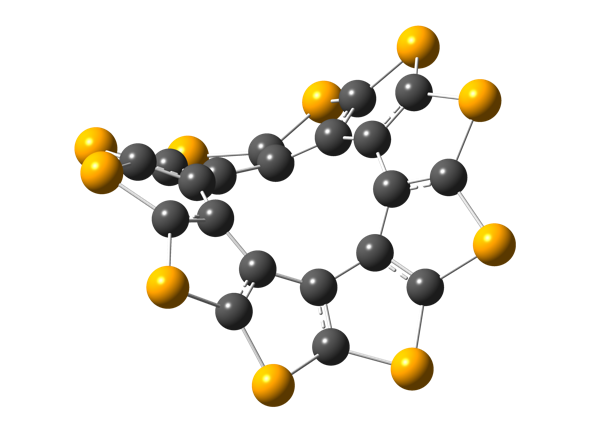
\includegraphics{se10}
    \caption[Se10 3D structure]{The 3D structure of Se10, the example molecule}
    \labfig{se10}
\end{marginfigure}

Se10, as well as all of the other sunflowers of the study, only contains heavy atoms that are relevant to the problem, so we can just ignore their chemical elements and treat every point equally.
However, it should be noted that in other cases there might be irrelevant atoms such as hydrogens, or parts of the molecule that don't belong to the surface that we are trying to identify.
In those situations, special care should be taken: the transformation operations have to be designed around the important atoms, but they should be applied to the whole system.

At this point, the relevant part of the molecule (i.e. the ring object of study), should be centered and aligned with the $z$ axis.
All of these preparatory steps ensure the optimal application of the actual method.

The method itself consists in the optimization of the coefficients of a multiple linear regression model.\marginnote{
	\begin{equation}
        \labeq{multiple-linear-regression}
        f_i \approx \beta_0 + \beta_1 x_{i1} + \beta_2 x_{i2} + ... + \beta_p x_{ip} \quad i=1,...,n
	\end{equation}
} %
A linear regression model with $p$ predictors and $n$ data points, as shown in \refeq{multiple-linear-regression}, consists of several elements.
$y$ is the target feature, the one that we wish to predict.
The various $x$ are the predictors, variables on which we base our predictions.
The various $\beta$ values are the coefficients that accompany the predictors and that we want to approximate.

In our case in particular, the bits of real data that we have -our ground truth- are the coordinates of the atoms of the molecule, which include $x$, $y$ and $z$ values.
Looking at it from the point of view of statistical learning, the problem could be defined as \q{designing a model that predicts the values of $z$ by using the values of $x$ and $y$}.
If such a model was developed, we could just input a square grid of $(x,y)$ values and get the height (or $z$ value) that they should be placed at to conform to our concept of general surface.
There is just a problem with this approach: using just $x$ and $y$ by themselves as the predictors is not enough to generate the kind of warped, wavy surfaces that we're looking for!
Just by adding different proportions of $x$ and $y$, the best one that we could get would be a tilted plane.%
\begin{margintable}
    \centering
    \caption[Calculated predictors]{Calculated predictors, with $f=\sqrt{(x^2+y^2)}$}
    \begin{tabular}{@{}S[table-format=1.4]
                       S[table-format=1.4]
                       S[table-format=1.4]
                       S[table-format=1.4]@{}}
        \toprule
        {$x^2$} & {$y^2$} & {$xy$} & {$f$} \\
        \midrule
        0.0230 & 1.8121 & 1.7809 & 3.3327 \\
        1.9680 & 0.9151 & 0.0901 & 0.3023 \\
        1.2690 & 0.0971 & 0.9504 & 1.3968 \\
        3.3270 & 1.0971 & 0.8505 & 1.3269 \\
        \multicolumn{4}{c}{{\ldots}}
    \end{tabular}
    \labtab{all-predictors}
\end{margintable}%
That is where the 3D surface selection approach gets mixed in.
We can combine the $x$ and $y$ values in certain ways in order to generate a wider variety of basic shapes to linearly combine, resulting in a better set of predictors.
For this problem, the following set of predictors was chosen: $x^2$ and $y^2$ (half cylinders, which result in a saddle when subtracted and a dome when added), $xy$ (a saddle aligned with the diagonal $x=y$), and $\sqrt{(x^2+y^2)}$ (a cone).\sidenote[][*9]{It should be noted that this is not proper statistical learning practice: in a real application the predictors shouldn't have any correlation between them.}

Having defined the elements of the model, its a matter of transforming the $x$ and $y$ values into their function forms, initializing a linear model, training it with these predictors and the values of the target variable $z$, and retrieving the coefficients.
This is all done using the convenient scikit-learn module,\sidecite{scikit-learn} a machine learning framework for the Python language.
Without delving deep in their lineal model's inner workings, it can be said that it relies on two key parts: a cost function that measures its deviation from the target, and an algorithm that minimizes it by iteratively modifying its coefficients.
When the model has been trained, its accuracy is measured by computing the values of the $R^2$ metric for two sets of points: the original coordinates of the atoms (i.e., the data points that the model is based on), and the middle points of each of the bonds (i.e. a collection of new data that the model hadn't previously known about).

All of this operations have been combined and encapsulated inside a custom Python command line application available in the author's GitHub account\sidecite{github-nics}.

Continuing with the running example, the output of the adjustment of Se10 would be as follows.
\begin{lstlisting}[label=se10-output, style=kaolstplain]
$ python nics.py surface se10.xyz

    Linear regression results:
                     x^2: -0.1056911
                     y^2:  0.1064271
                      xy:  0.1375246
         sqrt(x^2 + y^2): -0.0081293

    R2 score: 0.978916
    R2 score of atom midpoints: 0.988095
\end{lstlisting}

As a way of clearly displaying the result, the idea behind the method, and the elements of the linear combination, the functions have been plotted individually (omitting the last one due to its low contribution) in \reffig{linear-combination}.

\begin{figure*}
    \centering
    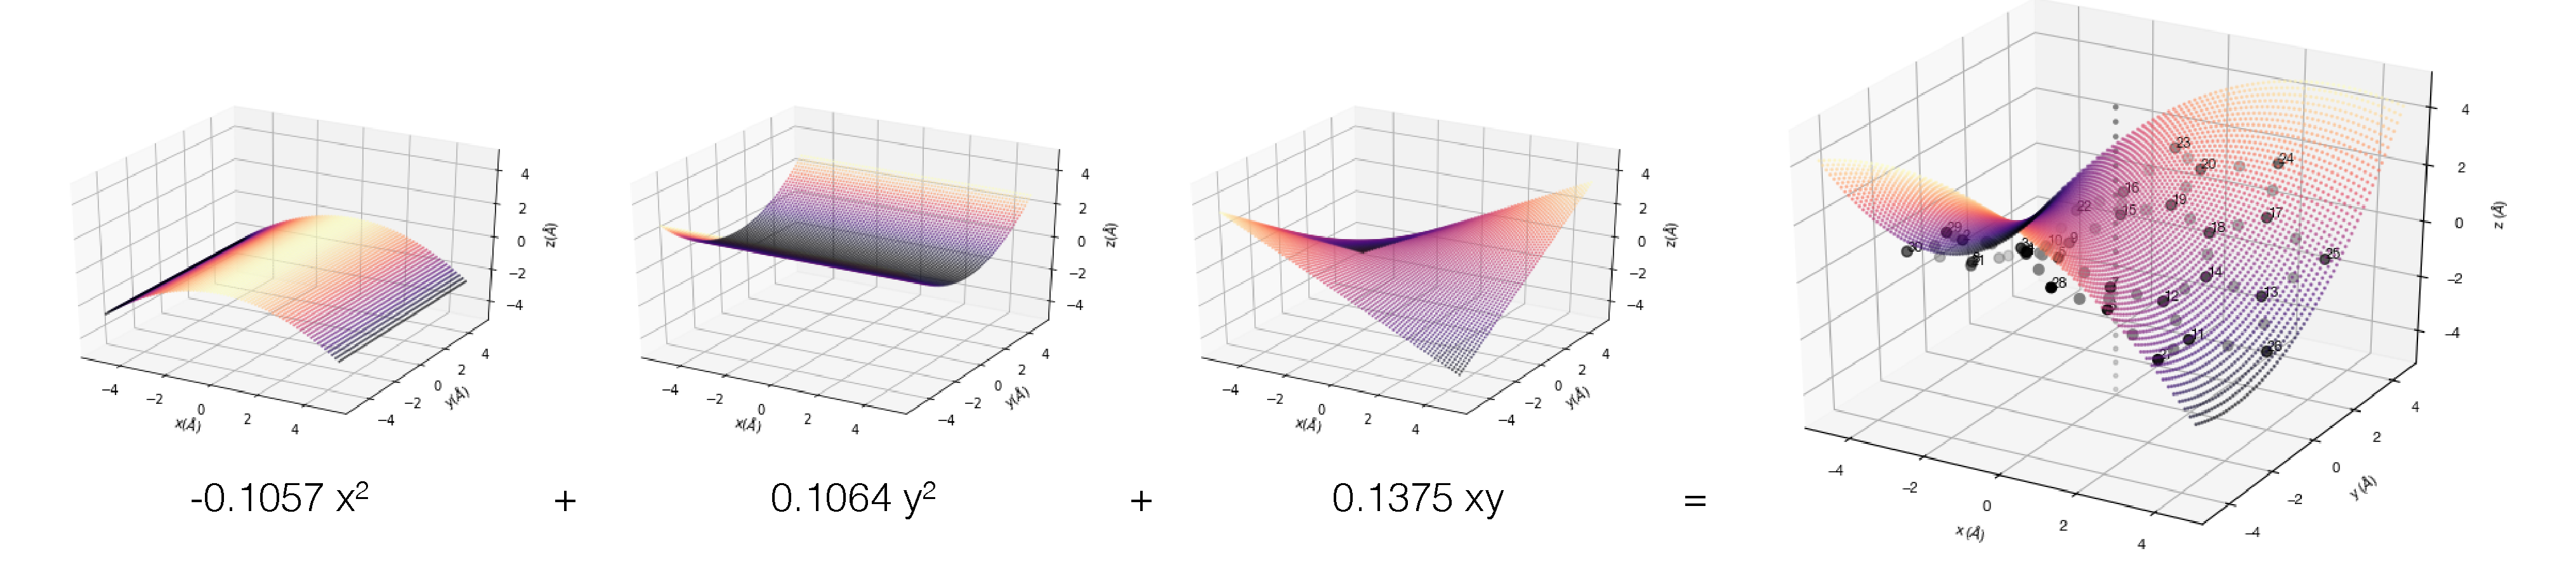
\includegraphics{linear-combination}
    \caption[Linear combination of base 3D functions]{Linear combination of base 3D functions to model the surface of Se10}
    \labfig{linear-combination}
\end{figure*}

After the surface has been defined, the results of the fitting are used to calculate a square grid of equally spaced points that are all equidistant to this molecule's surface.
In this case, a distance of \SI{1}{\angstrom} is set by general agreement with the literature.
Then, both the molecule atoms and the grid points are written into a Gaussian input file (the latter as dummy atoms), where the values of NICS will be calculated.
The calculation, specifically, estimates the values of the magnetic shielding using the Gauge-Independent Atomic Orbital (GIAO)\sidecite{keith93} method.

When the calculation is finished, the results can be visualized in 3D and plotted using the same program.
As it was previously said, through this technique aromatic compounds will experience shielding -negative values, marked in blue- on the inside of the ring and deshielding -positive values, marked in red- on the outside.
On the other hand, antiaromatic systems will experience the opposite effect.
This is the expected behavior and should be the basis for the evaluation of the technique, so to further verify it and illustrate it, the method has been applied to the well known model systems of benzene and cyclobutadiene.
Their 2D NICS graphs are included in \reffig{method-test}.

\begin{figure}[h]
    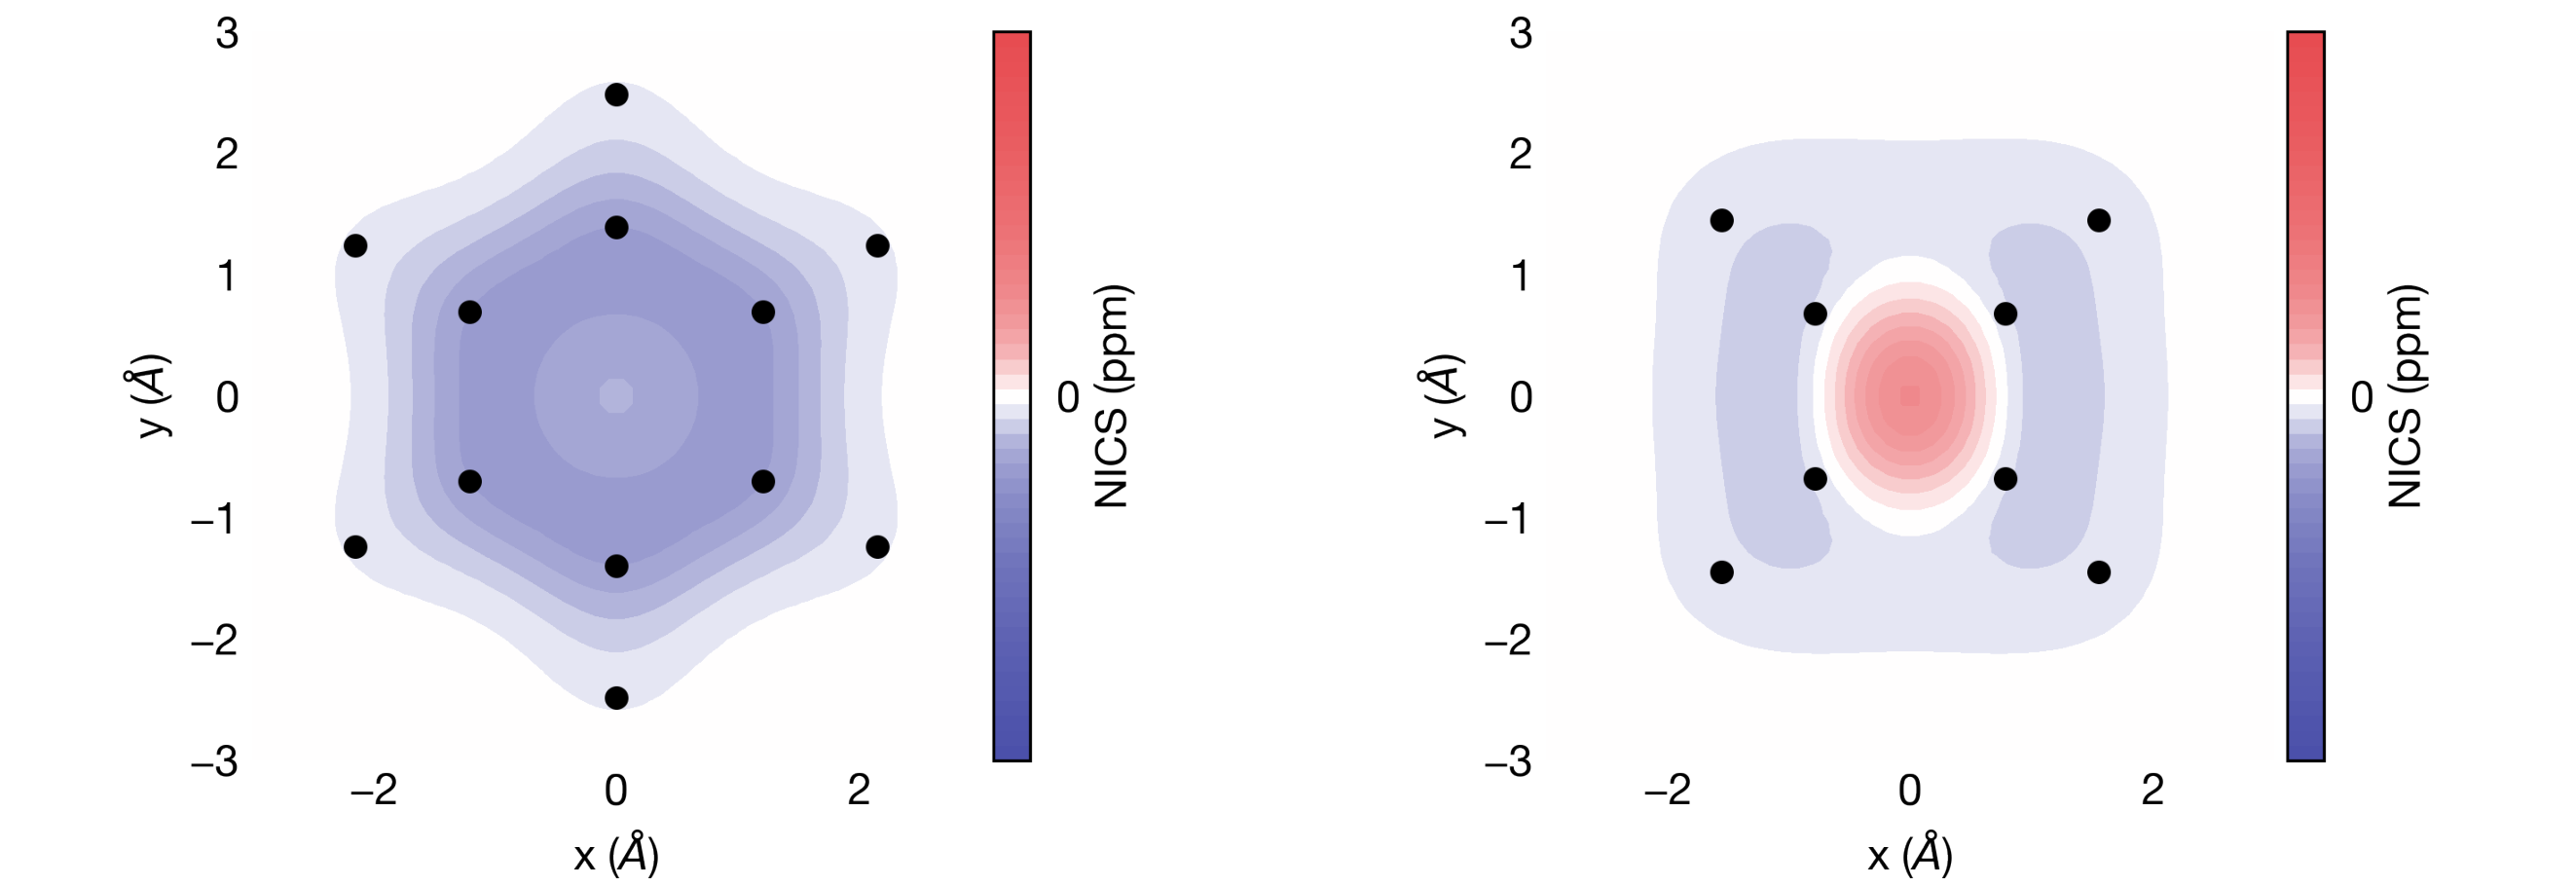
\includegraphics{method-test}
    \caption[NICS applied to test systems]{The custom NICS method, applied to benzene and cyclobutadiene from left to right}
    \labfig{method-test}
\end{figure}

The outcome for the Se10 calculation, plotted as a 2D projection onto the $xy$ plane, is displayed in \reffig{se10-2d}.
As it can be noted, all of the pentagonal rings that comprise the structure seem to have negative values of NICS, while only in the very center of the whole flower there seems to be a tendency towards positive values.
This hints that the Se10 flower may have aromatic characteristics from a magnetic point of view.
Complementing this insight with the geometry metrics summarized in \reftab{bond-length-study}, which indicated that all of the bonds of the same type had approximately the same distances, we could say that Se10 has an aromatic character.

\begin{marginfigure}
    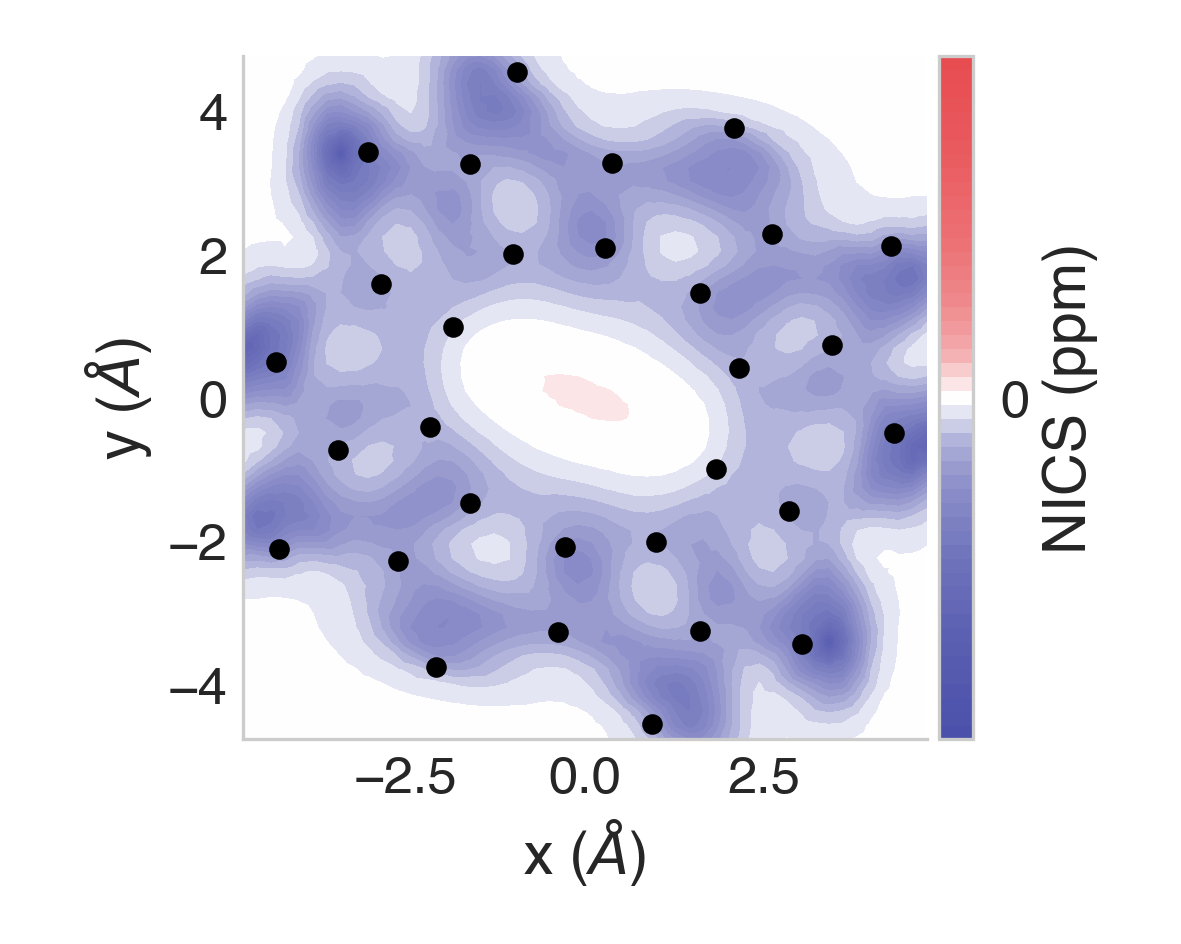
\includegraphics{se10-2d}
    \caption[NICS applied to Se10]{Custom NICS technique applied to the Se10 system}
    \labfig{se10-2d}
\end{marginfigure}%

On the other hand, let's take the example of the As08 molecule.
Its NICS projection, plotted in \reffig{as08-2d}, shows positive values all through the inside of all of the rings, with negative values on the outside of the whole structure.
This behavior is much more similar to that of cyclobutadiene than to that of benzene as shown in \reffig{method-test}.
These magnetic properties, in addition to the fact that the lengths of its bond groups had noticeably higher standard deviations, hint towards an antiaromatic character.

\begin{marginfigure}
    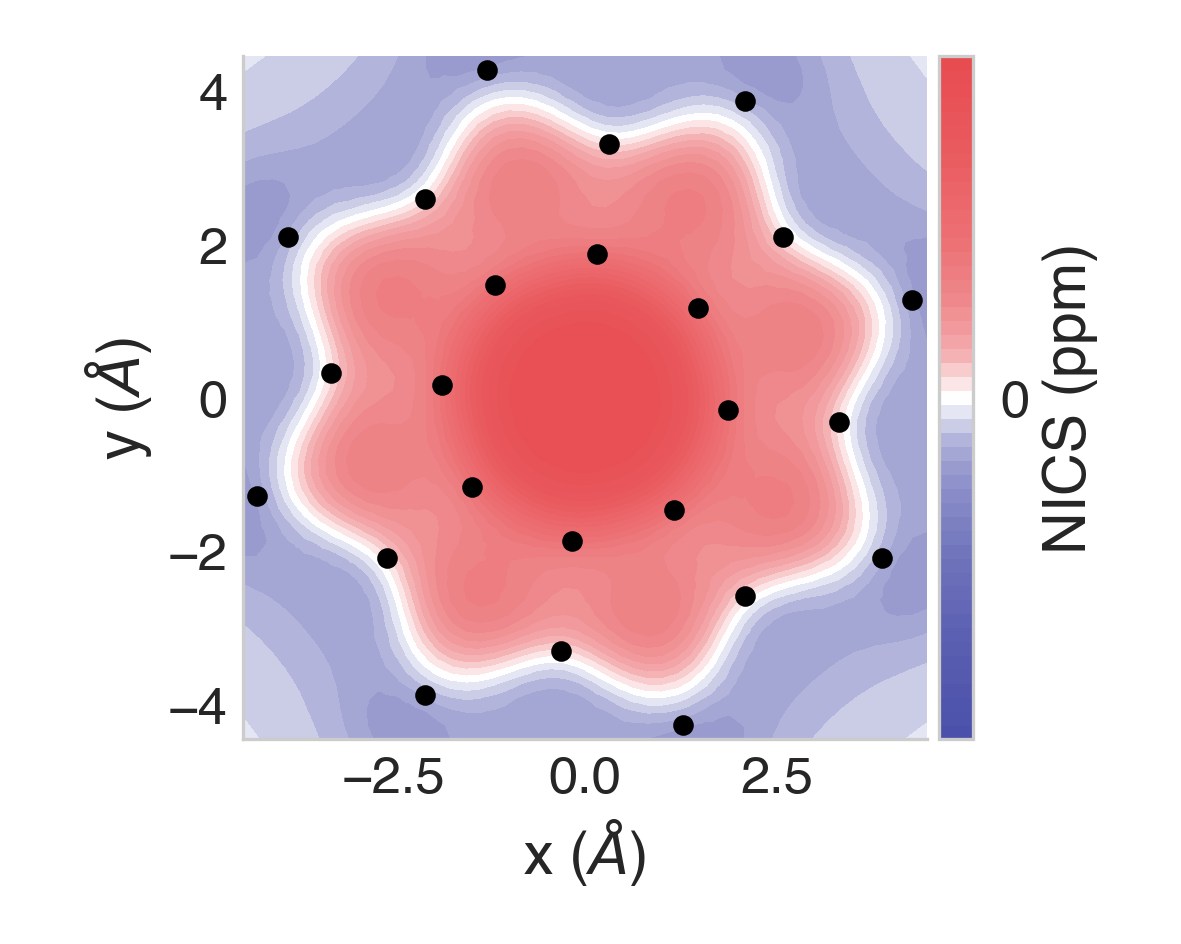
\includegraphics{as08-2d}
    \caption[NICS applied to As08]{Custom NICS technique applied to the As08 system}
    \labfig{as08-2d}
\end{marginfigure}

All of the NICS 2D projections for the rest of the flowers can be found in \refsec{ap:nics}, along with the corresponding comments interpreting each of them and proposing their most likely aromatic profile.
In general, two main conclusions were taken from the interpretation of these graphs.

First, only the As and P families presented magnetic profiles characteristic of antiaromaticity.
All of the other families had graphs similar to that of Se10: negative values of NICS all through the petals and only low positive values in the center, indicating signs of aromaticity.

Additionally, it was observed that the absolute values of NICS varied according to the number of petals depending on these proposed aromatic behaviors.
In aromatic families, the absolute value of the shielding increased as the number of petals did: S12 has larger NICS values than S08 (exemplified in \reffig{nics-s-family}).
However, in antiaromatic families, the largest absolute values were found in the flowers with the fewer petals.

\begin{figure*}
    \centering
    \begin{subfigure}{5.5cm}\centering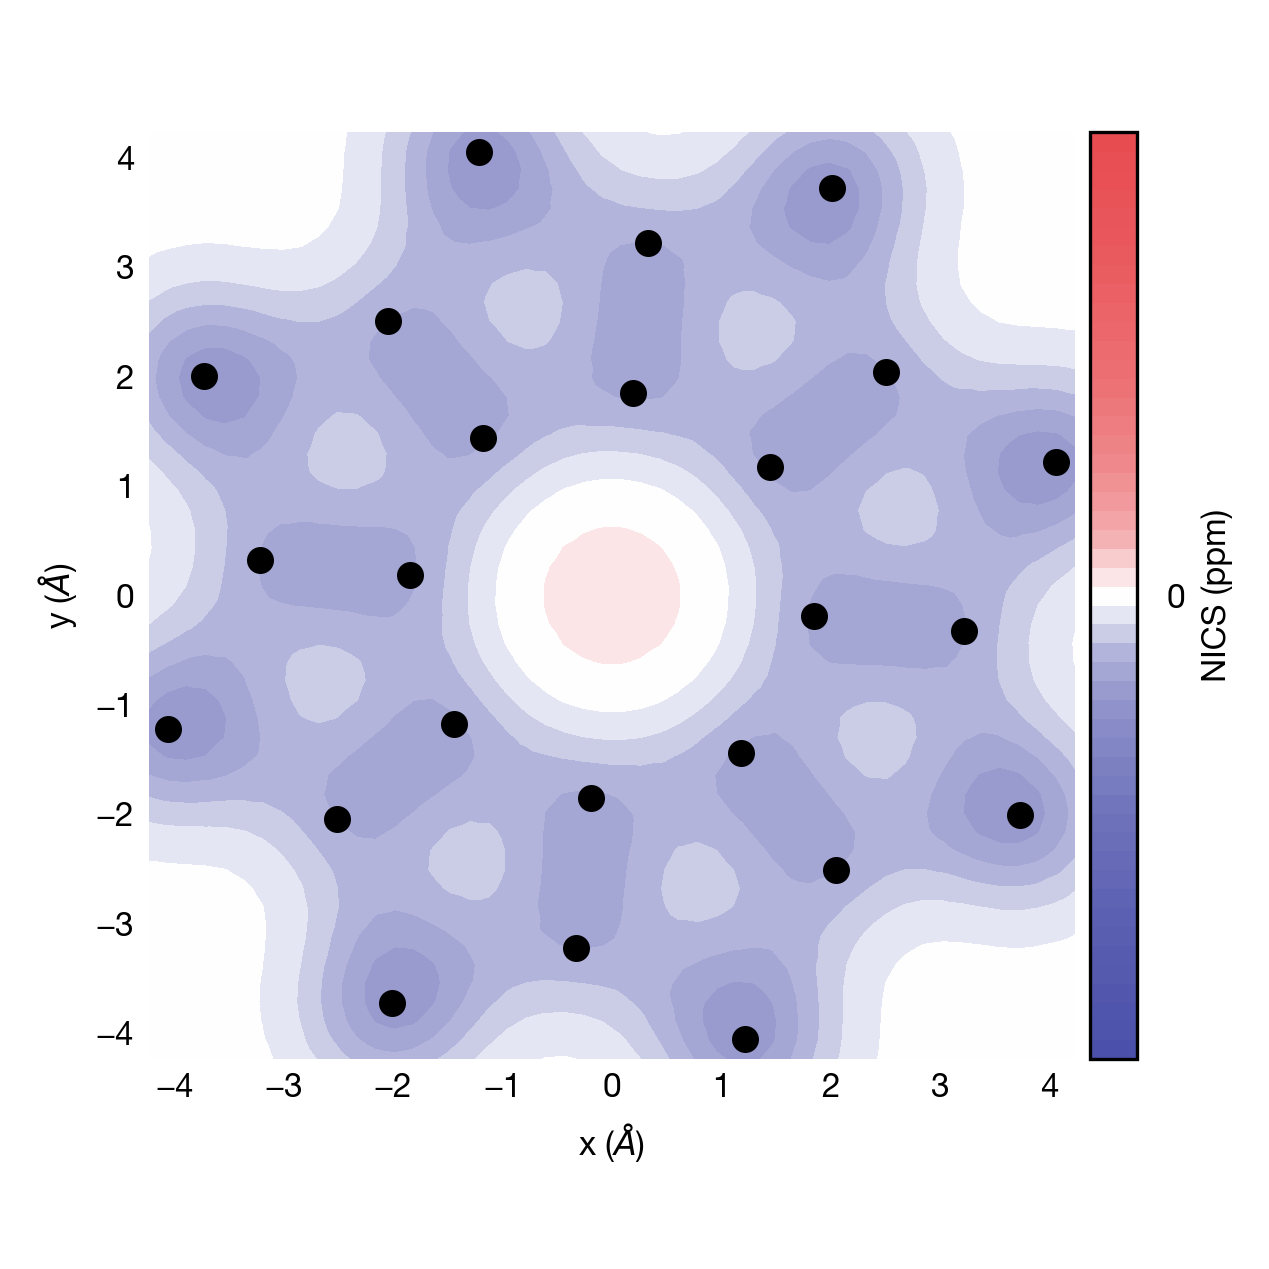
\includegraphics{s08-2d}\caption{NICS 2D projection for S08}\end{subfigure}%
    \begin{subfigure}{5.5cm}\centering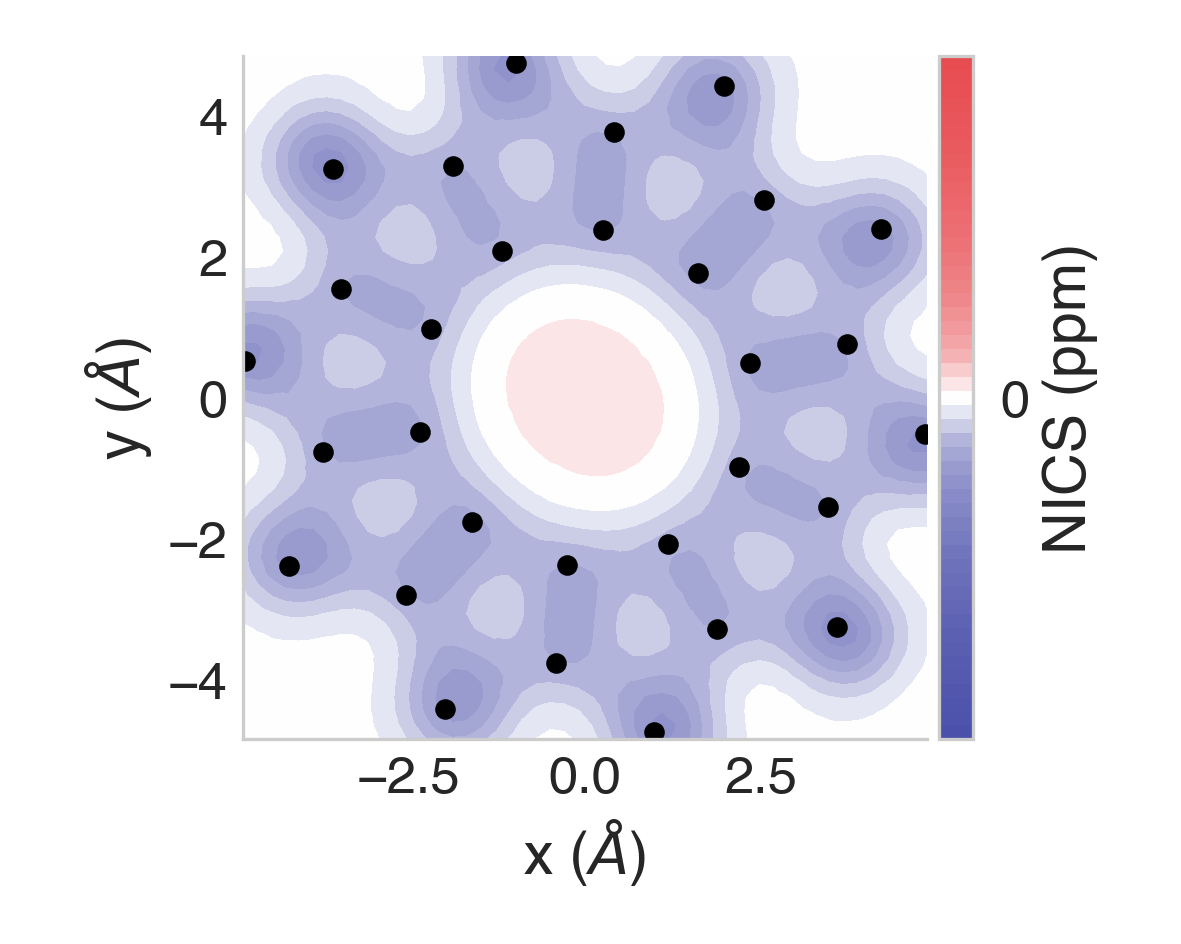
\includegraphics{s10-2d}\caption{NICS 2D projection for S10}\end{subfigure}%
    \begin{subfigure}{5.5cm}\centering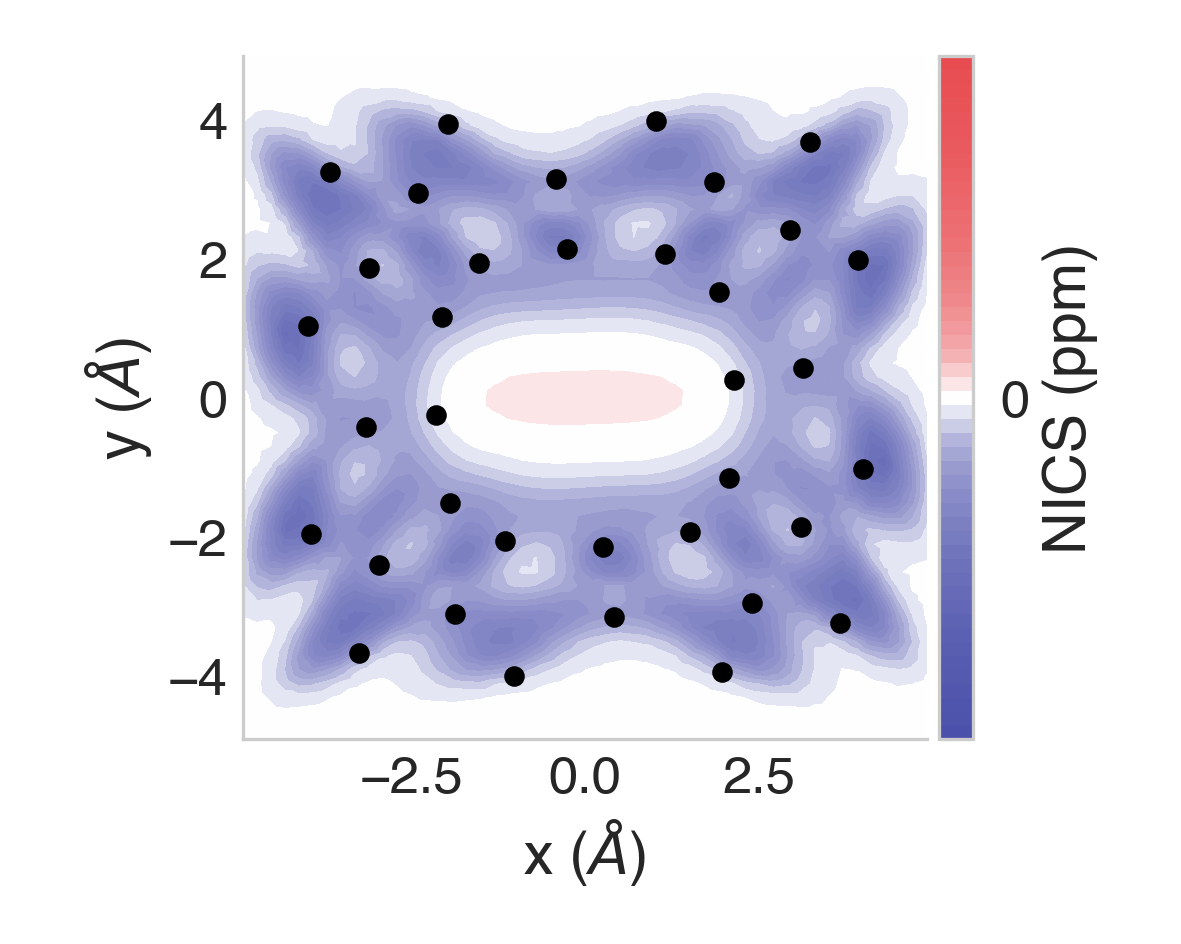
\includegraphics{s12-2d}\caption{NICS 2D projection for S12}\end{subfigure}
    \caption[NICS of S family]{NICS of the S family of flowers. Note the deeper blue values of NICS as the number of petals increases}
    \labfig{nics-s-family}
\end{figure*}

\section{Spectroscopic characterization}
After having obtained a general profile of the nature of this novel family of molecules, we start delving into the main topic of the work: spectroscopy.

\subsection{Vibrational spectroscopy}
\labsec{raman-flowers}
Sunflowers of 8, 10 and 12 petals have 66, 84 and 102 vibrational modes, respectively.\marginnote{Any non linear molecule with $N$ atoms has $3N-6$ vibrational normal modes}
Depending on whether these vibrations actively affect the dipole or the polarizability of the flowers, they can be detected using infrared spectroscopy, Raman spectroscopy, or both.
In this work we will focus on the vibrational modes that are visible through Raman spectroscopy, as previously discussed in \refsec{previous-work}.

\subsubsection{Raman spectra}
Raman spectra for all 18 sunflower systems were generated following the procedures detailed in \refsec{spectra-envelope-calculation}.

Their vibrational profiles were quite simple, but quite varied.
However, one specially characteristic vibrational mode was found common to all of them: the symmetric and simultaneous stretching ($\nu_\textit{s}$) of all of the middle bonds (those formed between X$_0$ and X$_2$ atoms).
These special vibrations, referred to as \q{A} modes from now on, are associated to clean high intensity peaks in the spectrum, and are therefore easily identifiable.
In all of the generated Raman spectra, the A mode has been plotted as a vertical dashed line.
Other vibrational modes that were also deemed important were plotted using vertical solid lines.
These other modes, while still characteristic and useful for the identification of the flowers, were not as clean or easily describable as A modes.
They involved mixtures of asymmetric scissoring ($\delta_\textit{as}$) of the inner (X$_0$-X$_0$) and outer (X$_1$-X$_2$) bonds, and the asymmetric stretching ($\nu_\textit{as}$) of inner and middle bonds.

Using the Raman spectra of some of the 8 petal flowers as an example, plotted in \reffig{flower-raman}, it can be observed that they always have present an A-type mode at fairly similar frequencies.

\begin{figure*}[h]
    \centering
    \begin{subfigure}{8.25cm}\centering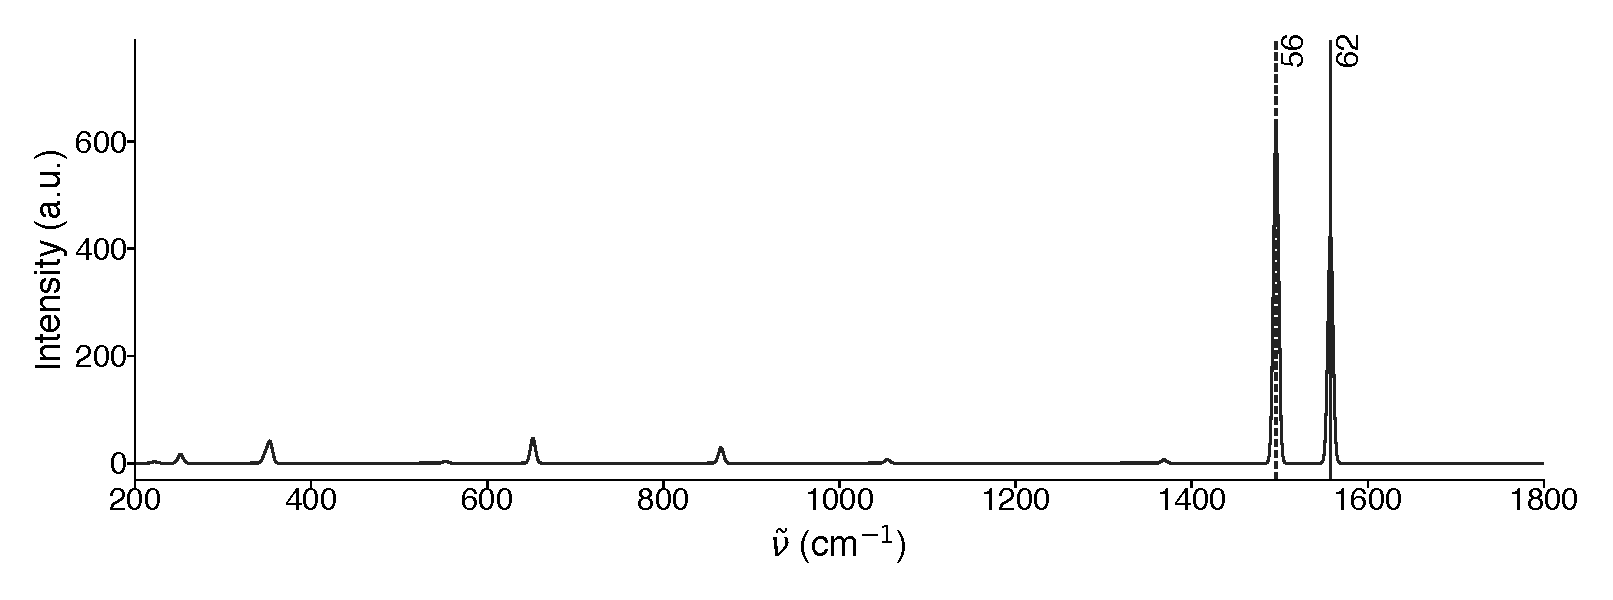
\includegraphics{raman-s08}\caption{Raman spectrum for S08}\end{subfigure}%
    \begin{subfigure}{8.25cm}\centering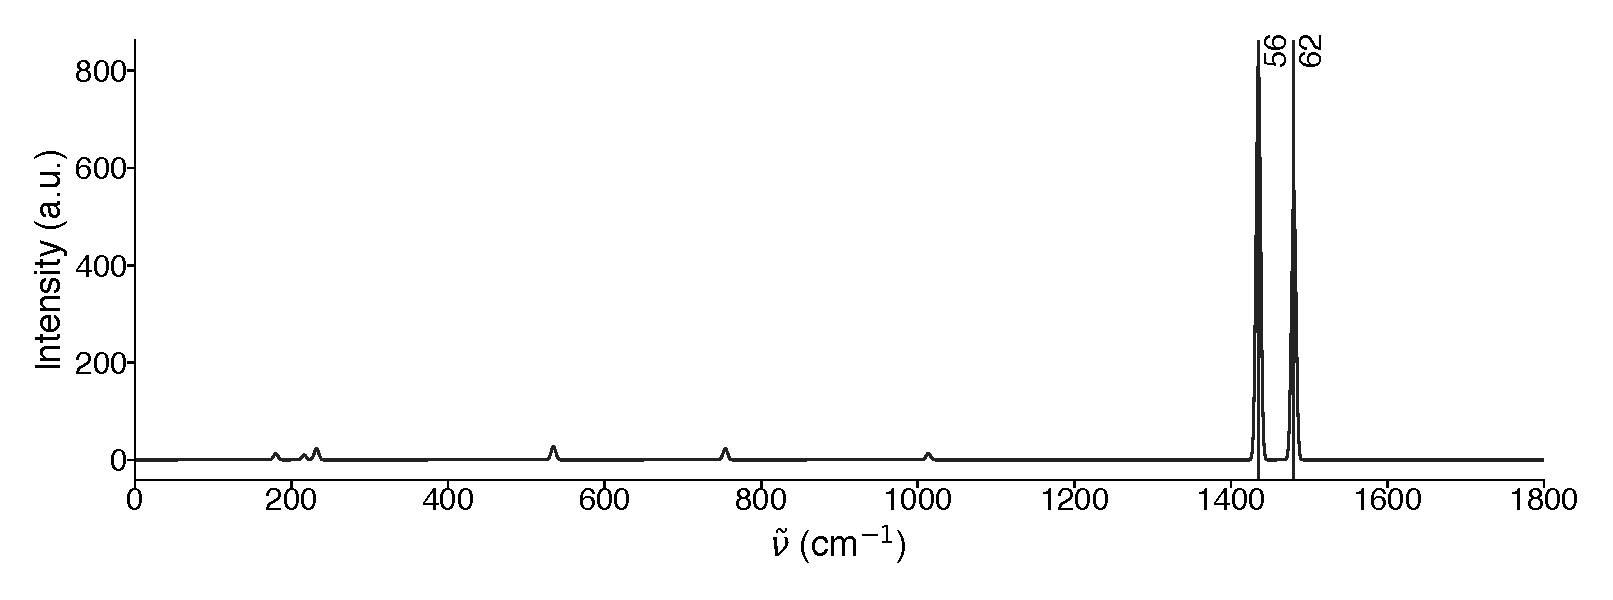
\includegraphics{raman-se08}\caption{Raman spectrum for Se08}\end{subfigure}
    \begin{subfigure}{8.25cm}\centering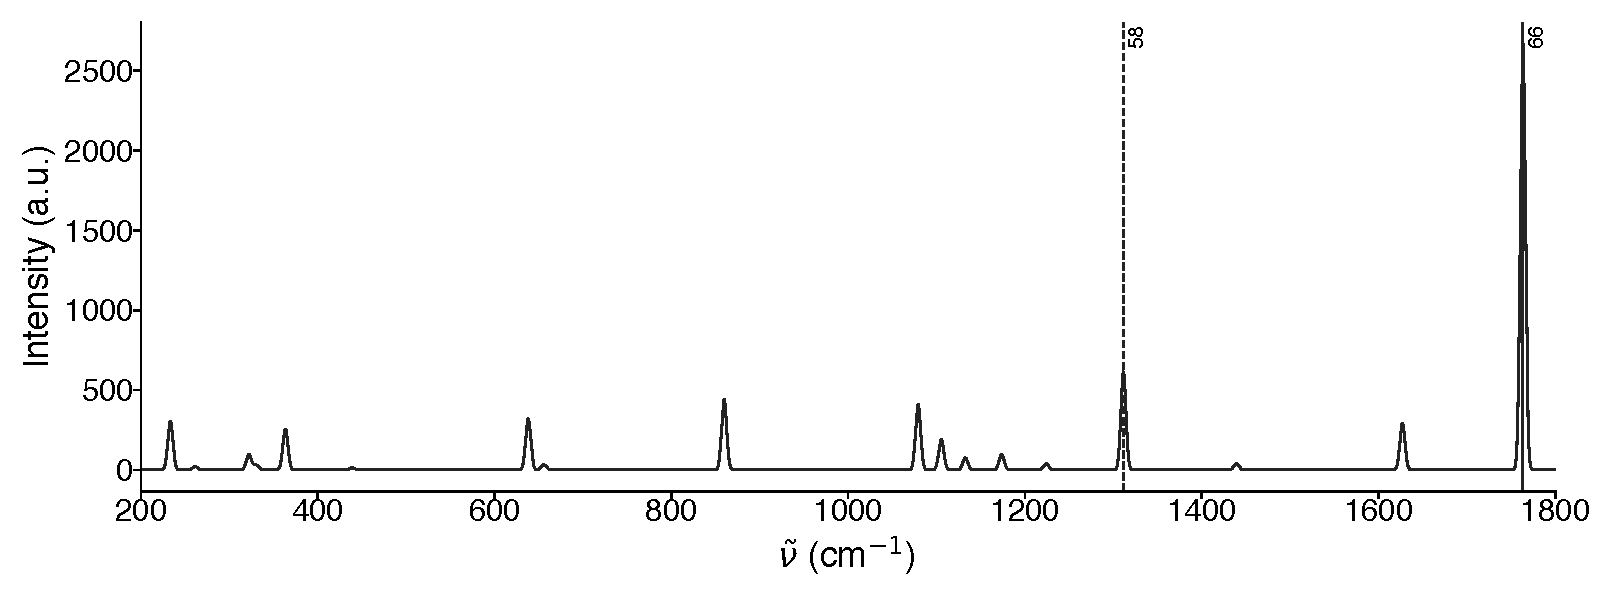
\includegraphics{raman-p08}\caption{Raman spectrum for P08}\end{subfigure}%
    \begin{subfigure}{8.25cm}\centering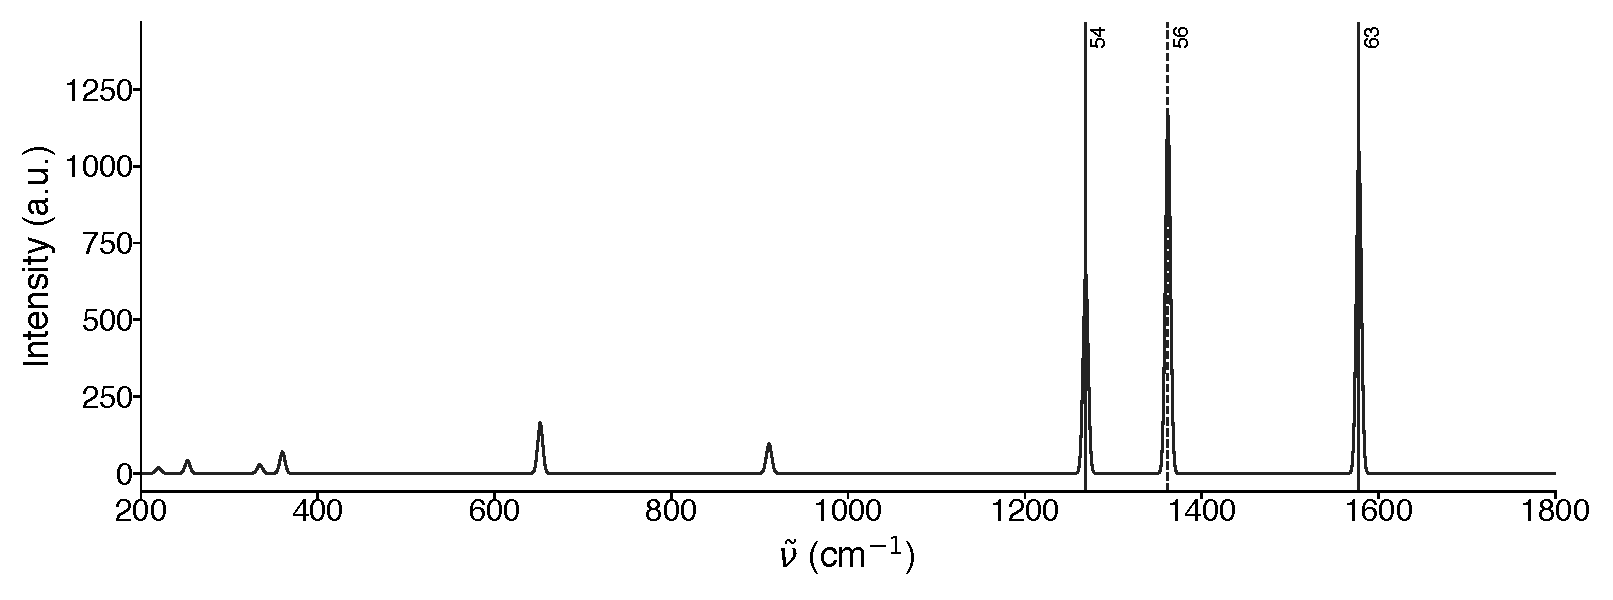
\includegraphics{raman-pn08}\caption{Raman spectrum for PN08}\end{subfigure}
    \caption[Raman spectra of 8 petal flowers]{Raman spectra of a selection of 8 petal flowers. Note the A modes plotted with dashed lines}
    \labfig{flower-raman}
\end{figure*}

Additionally, in general, an increase in the complexity of the spectra and a decrease in the cleanliness of the spectra was observed alongside the increase of the number of petals: flowers with 12 petals had more complex patterns of modes than flowers with 8.

Let's take, for example, the As family.
The spectra for As08 and As12, displayed  in \reffig{as-raman}, have clear differences in intricacy and number of modes.

\begin{figure*}[h]
    \centering
    \begin{subfigure}{8.25cm}\centering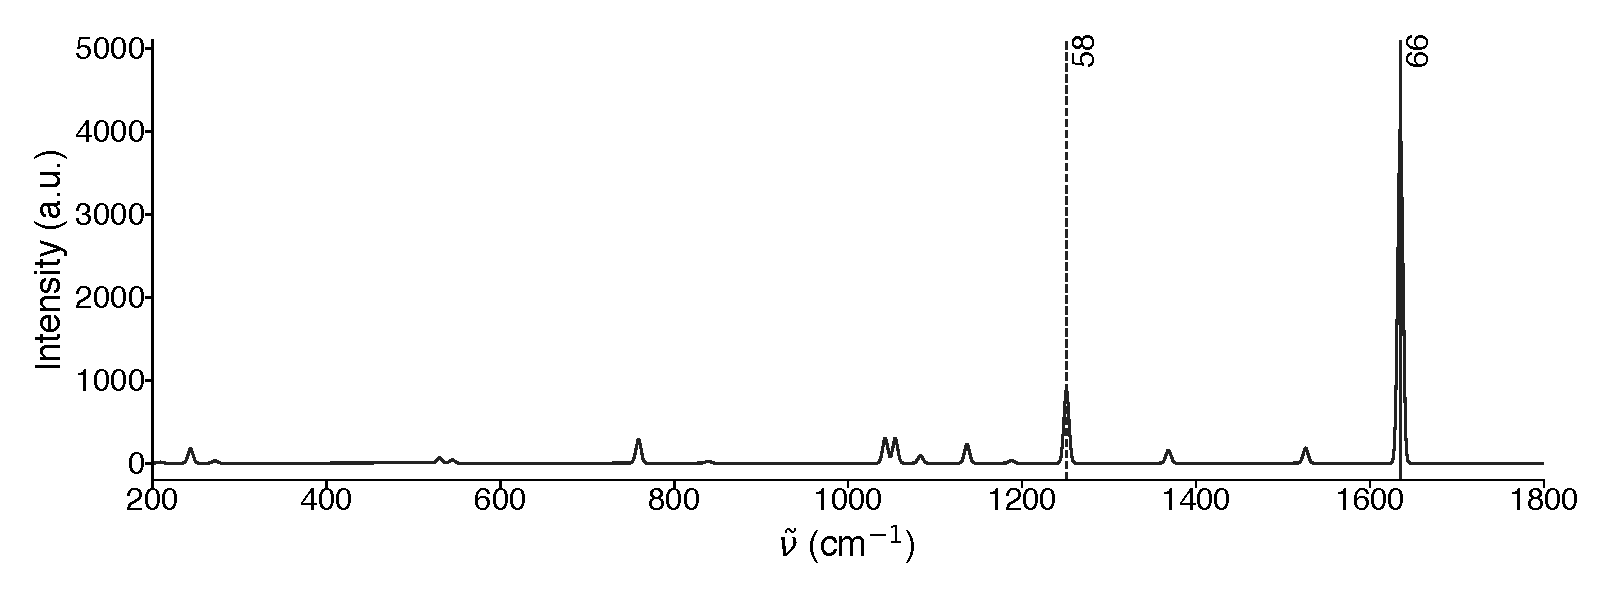
\includegraphics{raman-as08}\caption{Raman spectrum for As08}\end{subfigure}%
    \begin{subfigure}{8.25cm}\centering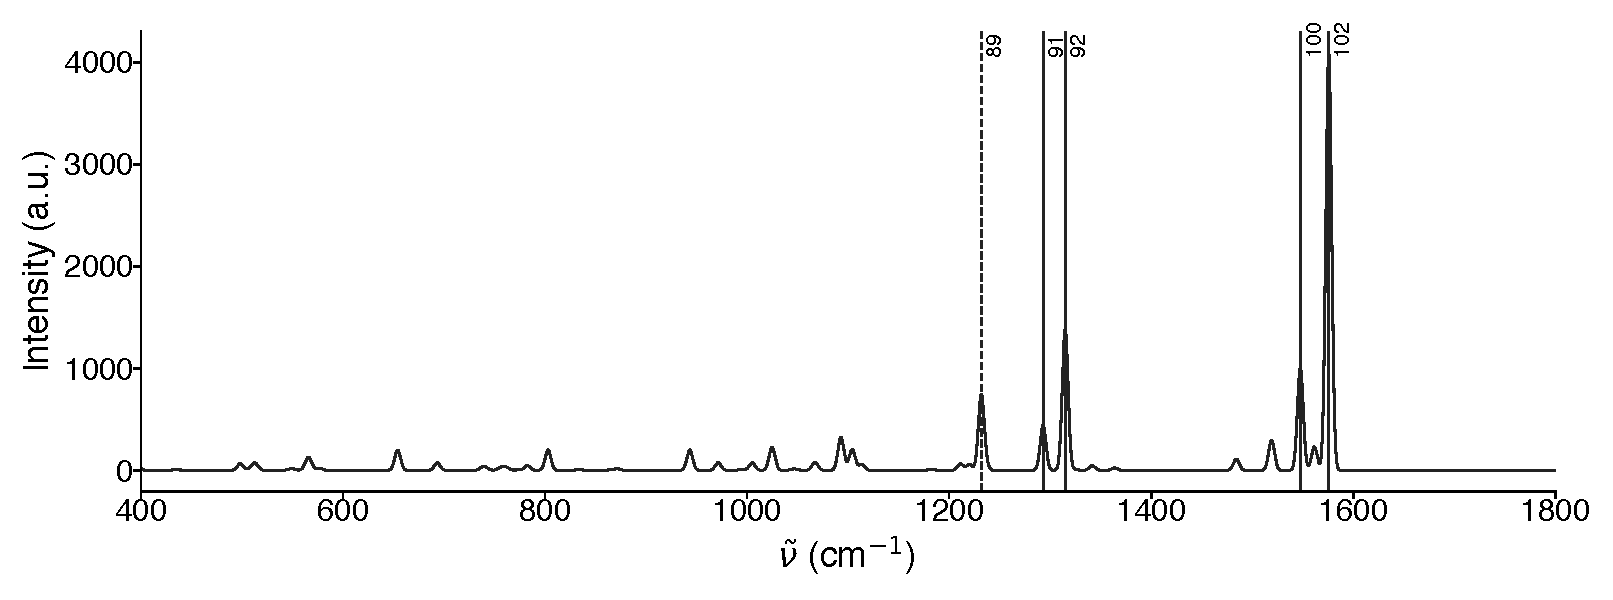
\includegraphics{raman-as12}\caption{Raman spectrum for As12}\end{subfigure}
    \caption[Raman spectra of As08 and As12]{Raman spectra of As08 and As12}
    \labfig{as-raman}
\end{figure*}

All in all, these spectra were considered simple and clear enough to allow for the identification of the flowers.
The other spectra that weren't displayed in this section can be found in \refsec{ap:raman-flowers}.

\subsection{Electronic spectroscopy}
\labsec{uv-sunflowers}
Keeping in mind the final objectives of the work of applying resonance Raman, the electronic spectroscopic behavior of the flowers was deemed as a relevant point to study: the characterization of the electronic transitions of a molecule might yield insight about its interactions with light.

\subsubsection{UV-vis spectra}
The most straightforward way to study electronic spectroscopy is by simulating ultraviolet-visible (UV-vis) spectra.
In order to generate this, the energies of the 50 first transitions from the ground state to excited states were computed using TD-DFT in the Gaussian09 suite.
Then, using their energy and oscillator strength values, Gaussian functions were calculated for each of the transitions and linearly combined to create continuous spectra similar to those obtained using real spectrophotometers.
This procedure is further explained in \refsec{spectra-envelope-calculation}.
UV-vis spectra were generated for all of the sunflowers, but since they are fairly simple graphs, only the one for S08 will be explained in this section as an example.
It's displayed in \reffig{uv-s08-simple}.

\begin{figure}[h]
    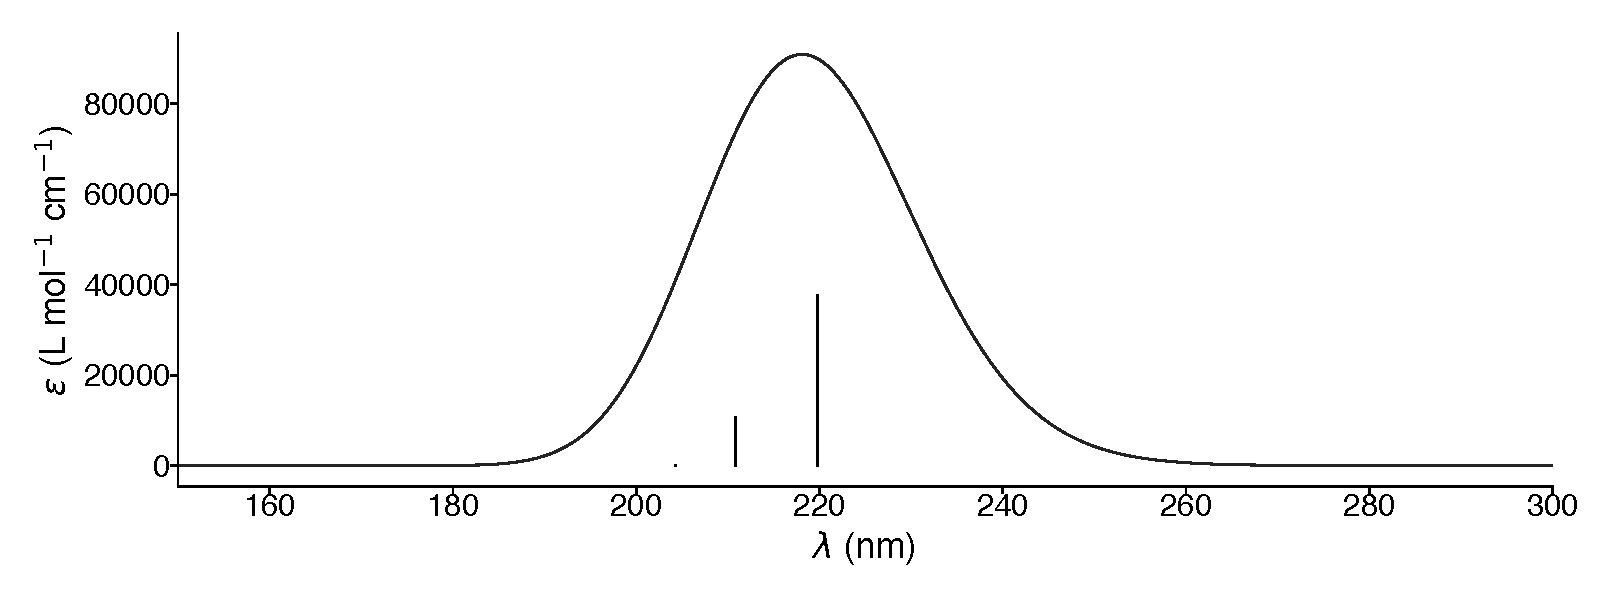
\includegraphics{uv-s08-simple}
    \caption[UV-vis spectrum of S08]{UV-vis spectrum of S08}
    \labfig{uv-s08-simple}
\end{figure}

\begin{margintable}
    \centering
    \caption[UV-vis absorption range of isolated flowers]{Approximate UV-vis absorption range of isolated flowers}
    \begin{tabular}{@{}rc@{}}
        \toprule
        System & $\lambda$ (\si{\nano\metre}) \\
        \midrule
        S08 & 180-260 \\
        S10 & 180-280 \\
        S12 & 200-400 \\
        Se08 & 200-280 \\
        Se10 & 200-400 \\
        Se12 & 225-500 \\
        As08 & 250-800 \\
        As10 & 250-700 \\
        As12 & 300-900 \\
        AsN08 & 300-450 \\
        AsN10 & 300-650 \\
        AsN12 & 300-850 \\
        P08 & 225-700 \\
        P10 & 250-500 \\
        P12 & 250-700 \\
        PN08 & 250-500 \\
        PN10 & 250-550 \\
        PN12 & 300-700 \\
    \end{tabular}
    \labtab{flower-uv-ranges}
\end{margintable}

We can see that the spectrum for S08 goes from \SI{190}{\nano\metre} to \SI{260}{\nano\metre}, approximately.
Plotted as straight vertical lines, the individual electronic transitions have been included, where their height is proportional to their oscillator strength.
However, this is not an adequate representation in this case.
What appear to be 2 electronic transitions located at \SI{210}{\nano\metre} and \SI{219}{\nano\metre} are, in fact, 4 different transitions (specifically, there are 2 groups of 2 each): it's just that due to the high symmetry of the molecule, transitions that occur in regions of the molecule that are very electronically similar might have coinciding wavelengths.

This was true for most of the flowers: many of the transitions with the higher intensities were grouped in pairs.
The only cases where this effect didn't clearly happen were the sunflowers with the most warped and most bent geometries, such as As12, AsN12, P12 and PN12.

In any case, since the purpose of studying individual electronic transitions is to serve as a guide when applying resonance techniques and we won't study the resonance of the isolated flowers, they were left out of the spectra.

The rest of the UV-vis spectra of the flowers may be found in \refsec{ap:uv-vis-flowers}.
Their absorption ranges, nonetheless, have been summarized and presented in \reftab{flower-uv-ranges} as an overview.

\section{Conclusions}

Summarizing this whole chapter into a list of important points:

\begin{itemize}
    \item The family of molecules of the study, collectively named as \q{flowers} or \q{sunflowers}, was built using molecules based on \q{sulflower} using S, Se, As, As+N, P and P+N as substituents.
    \item Flowers with 8, 10 and 12 petals were generated due to their higher structural and electronic stability, resulting in a total of 18 different molecules.
    \item Statistical analysis was performed on the length of their bonds, and the values of their mean and standard deviation were considered as early indicatives of their stability and their possible conjugation effects.
    \item The strain energy for each flower was calculated through the design of a homodesmotic reaction.
    \item Aromaticity was directly studied using an approach designed and programmed by the author using multiple linear regression and NICS. It was found that all flower groups except for As and P exhibited magnetic behavior that hinted towards aromatic character.
    \item The Raman active vibrational modes of the flowers were briefly characterized and plotted as Raman spectra.
    \item The electronic spectroscopy of the flowers was studied by generating their UV-vis spectra.
\end{itemize}

All in all, all of the studied flowers were considered stable and interesting enough to be applied to the STX problem as surface-like adsorption substrates.

\setchapterimage[2cm]{../images/header-stx.png}
%\setchapterpreamble[u]{\margintoc}
\chapter{Study of sunflower-saxitoxin complexes}
\labch{stx}

\begin{marginfigure}
    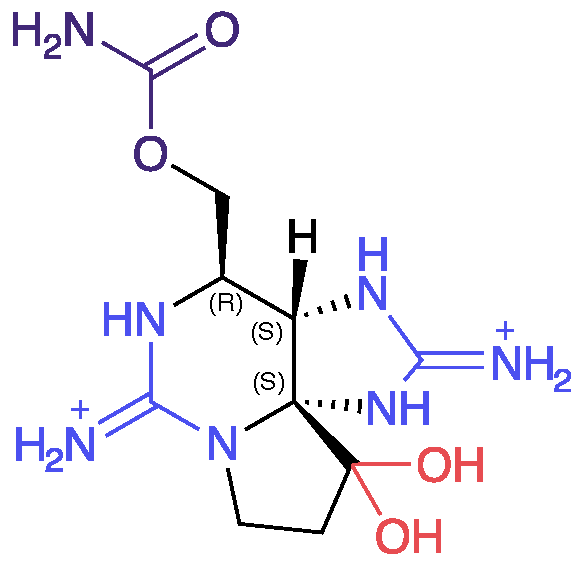
\includegraphics{stx-structure}
    \caption[Functional groups of STX]{Functional groups of STX}
    \labfig{stx-structure}
\end{marginfigure}

Having obtained a general characterization of the sunflower-type molecules and their spectroscopy, it was time to get back to the problem at hand and start looking into how they can be applied.

Let's reintroduce the molecule that motivated this whole study: saxitoxin (STX).
For the purposes of this study, the STX structure features two guanidinium moieties (which are easily susceptible to protonation and are marked in blue), two hydroxyl (in orange), and one carbamate group (in green) as it can be seen in \reffig{stx-structure}.

The STX being doubly protonated in the figure is not an arbitrary choice.
While studying its acid-base behavior in previous work we faced a certain issue: the STX molecule has many possible protonated variations, and at the pH of real life samples there would be a coexistence of several of them.
This was a problem, because having to apply the study to these different multiple forms in order to account for the situation would greatly increase the number of calculations.
After some thought, it was decided that the simplest way to solve this issue would be to work at a pH where only one of the protonated species would be present at a significant amount.
It was found that, at the moderate pH value of 6, the majority of the STX could be found as its doubly protonated form.
Since in real life experimental conditions attaining a pH of 6 in an hypothetical water-based sample would only imply the addition of a few drops of dilute acid, it was decided that all further studies would be carried out using such diprotonated structure.

\section{Spectroscopic study of lone STX}
The goal of this work was presented as \q{finding suitable substrate to aid in the detection of STX} from the beginning, but this desire came from a place of previous study and understanding about the spectroscopic properties of the lone STX.

This section aims to display and share the most important of these previously known facts, which are about the behavior of saxitoxin in both vibrational and electronic spectroscopy contexts.

\subsection{Vibrational spectroscopy}
As a non linear molecule with 40 atoms, STX presents a total of 114 vibrational normal modes.
Many of those modes cause changes in its polarizability, and are therefore visible in its Raman spectrum.
In this section, we pinpoint and describe a selection of the most characteristic and noticeable vibrational modes that could allow for the identification of the isolated STX.

\subsubsection{Raman spectrum}
The Raman spectrum of STX was calculated and plotted in the same way as those of the sunflowers, and displayed in both \reffig{raman-stx} and \ref{fig:raman-stx-zoom}.

\begin{figure}
    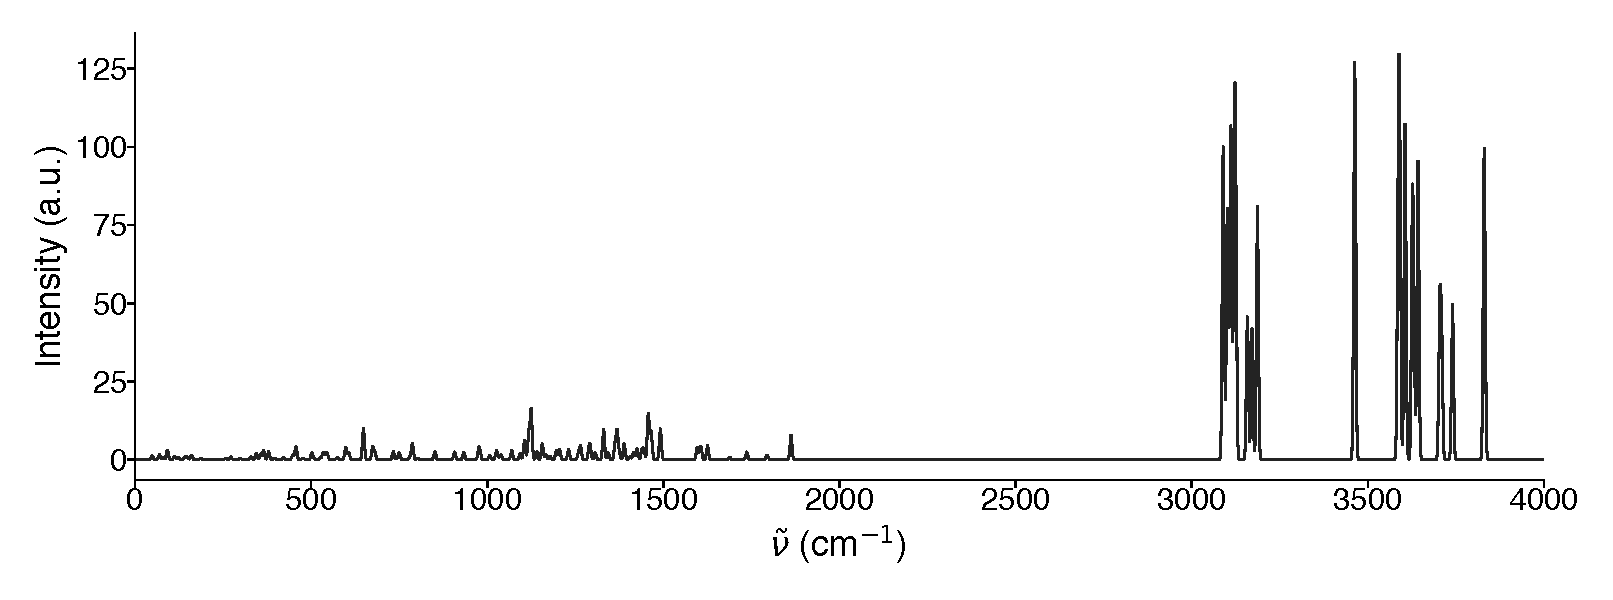
\includegraphics{raman-stx}
    \caption[Raman spectrum of lone STX]{Raman spectrum of lone STX}
    \labfig{raman-stx}
\end{figure}

\begin{figure*}
    \begin{subfigure}{8.25cm}\centering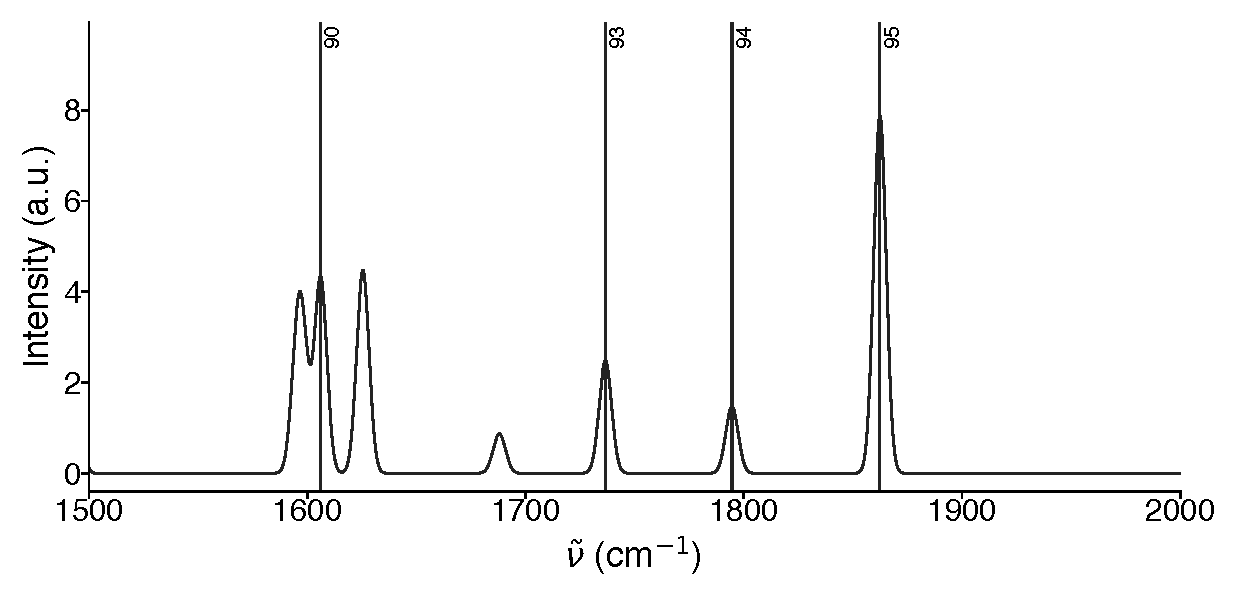
\includegraphics{raman-stx-left}\end{subfigure}%
    \begin{subfigure}{8.25cm}\centering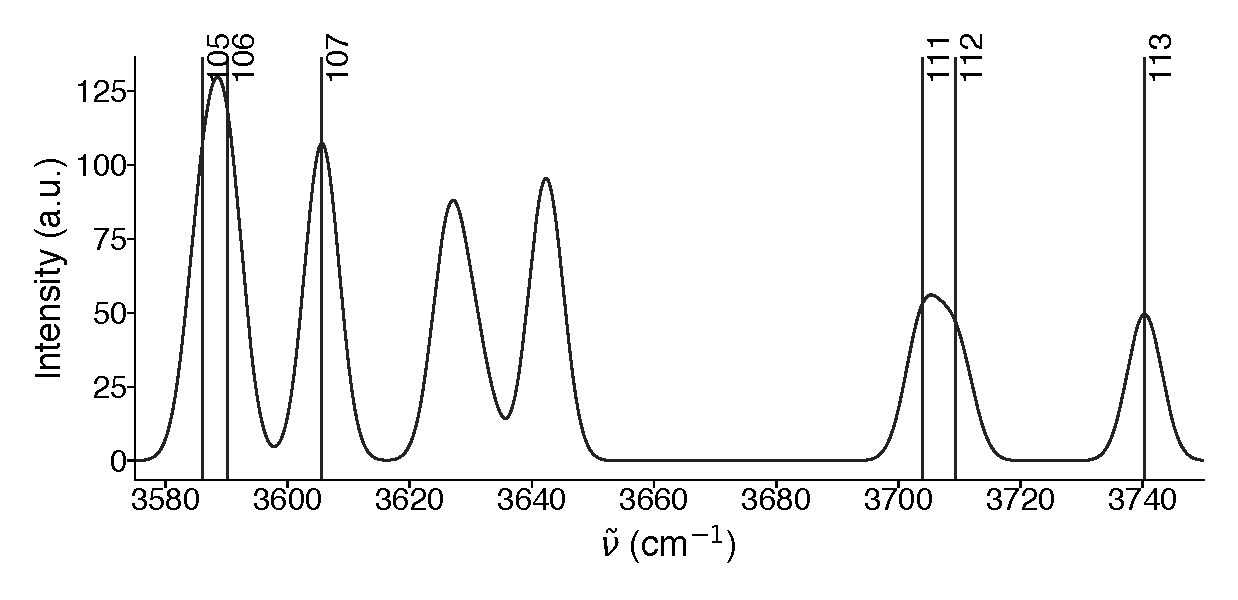
\includegraphics{raman-stx-right}\end{subfigure}
    \caption[Zoomed in Raman spectrum of lone STX]{Zoomed in Raman spectrum of lone STX with annotated vibrational modes}
    \label{fig:raman-stx-zoom}
\end{figure*}

\begin{table}
    \caption[Raman modes of STX]{Selected Raman active vibrational modes for STX. Letters $\delta$ and $\nu$ are scissoring and stretching vibrations; subscripts $_\textit{s}$ and $_\textit{as}$ mean symmetric and antisymmetric; and G5, G6 and Cb are the 5 atom guanidinium moiety, the 6 atom guanidinium moiety, and the carbamate group.}
    \labtab{stx-modes}
    \begin{tabular}{@{}rS[table-format=4.1]r@{}}
        \toprule
        Mode & {$\tilde{\nu}$} & Description \\
        \midrule
        90 & 1606.2 & $\delta_s$ \ce{NH2} G5 \\
        91 & 1625.5 & $\delta_s$ \ce{NH2} G5 \\
        93 & 1736.6 & $\delta_s$ \ce{NH2} G6 \\
        94 & 1794.6 & $\delta_s$ \ce{NH2} G5 \\
        95 & 1862.4 & $\delta_s$ \ce{NH2}, $\nu_\textit{as}$ \ce{OCN} Cb \\
        105 & 3586.1 & $\nu_\textit{s}$ \ce{NH2} G5 \\
        106 & 3590.2 & $\nu_\textit{s}$ \ce{NH2} G6 \\
        107 & 3605.6 & $\nu_\textit{s}$ \ce{NH2} Cb \\
        111 & 3704.0 & $\nu_\textit{as}$ \ce{NH2} G5 \\
        112 & 3709.4 & $\nu_\textit{as}$ \ce{NH2} G6 \\
        113 & 3740.3 & $\nu_\textit{as}$ \ce{NH2} Cb \\
        \bottomrule
    \end{tabular}
\end{table}

These annotated modes, specified and described in \reftab{stx-modes}, were deemed as sufficient to identify the lone STX in a sample.
This is a good exercise to start identifying characteristic vibrations that could be attributed to STX.
However, it must be kept in mind that this analysis only serves as an initial approximation, as it's possible that these same vibrational modes have shifted wave numbers and/or are different when the STX gets adsorbed and forms complexes.

\subsection{Electronic spectroscopy}
\labsec{uv-stx}
STX doesn't have any special chromophore groups, and its excited states are available at the UV range of electromagnetic radiation.
Nevertheless, it's important to identify and study these transitions in order to facilitate the application of further techniques.

\subsubsection{UV-vis spectrum}
As before, using TD-DFT as implemented in Gaussian09, the first 50 electronic transitions were calculated and used to generate the UV-vis spectrum of STX, displayed in \reffig{uv-stx}.

\begin{figure}
    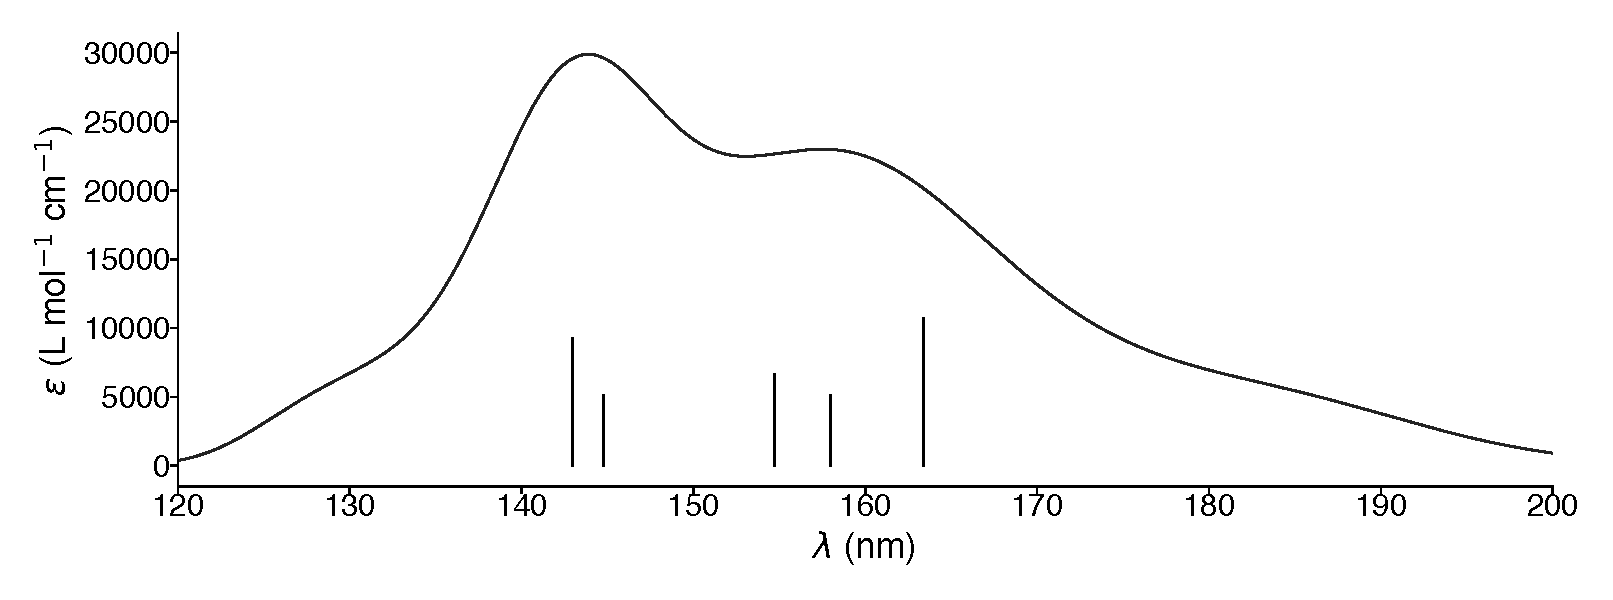
\includegraphics{uv-stx}
    \caption[UV-vis spectrum of lone STX]{UV-vis spectrum of lone STX, the 5 electronic transitions with the largest contributions have been annotated}
    \labfig{uv-stx}
\end{figure}

As it may be noted, the range of absorption (between \SI{120}{\nano\metre} and \SI{200}{\nano\metre}) is located within the UV region.
As discussed previously in \refsec{previous-work}, it's possible to induce resonance Raman effects at this wavelengths, it's just that it's expensive and impractical to use lasers that energetic in real experimental settings.
This range of UV-vis absorption need to be shifted to allow for the usage of more common incident laser wavelengths.

\section{Study of adsorption}

Having characterized the spectroscopic profile of STX, it's time to assess its interactions with the members of the sunflower family, keeping in mind the goal of determining if any of them could be a substrate suitable for its detection.
The first study that must be carried out, before any spectroscopic technique can be applied, is that of adsorption: how does STX adhere to the flowers, how stable the resulting complex is...
This is a crucial matter, as there's no point in calculating spectra for a system that isn't stable.

\subsection{Sampling and optimization}

\begin{margintable}
    \centering
    \caption[Energies of S08-STX conformers]{Relative energies of the S08-STX conformers, with respect to the most stable one}
    \begin{tabular}{@{}l
                       S[table-format=2.3]@{}}
        \toprule
        System ID & {Rel. E (\si{\kilo\calorie\per\mole})} \\
        \midrule
        S08-STX-1 & 0.000 \\
        S08-STX-2 & 1.337 \\
        S08-STX-9 & 7.133 \\
        S08-STX-7 & 7.504 \\
        S08-STX-6 & 9.896 \\
        S08-STX-4 & 18.554 \\
        S08-STX-3 & 20.321 \\
        S08-STX-10 & 21.734 \\
        S08-STX-5 & 22.529 \\
        S08-STX-8 & 29.715 \\
    \end{tabular}
    \labtab{stx-s08-energies}
\end{margintable}

In order to take into account the possible conformational variability, the STX was manually given an array of different relative positions and angles with respect to the surface of the flowers.
Following this idea, 10 different variations were modeled for each of the 18 sunflower-STX pairs, resulting in a total of 180 structures.
These various orientations will be referred to as \q{conformers}.
All of the conformers for each pairing were optimized at the M06-2X/def2SVP calculation level, and their final energies were compared in order to identify the most stable ones and discard the unstable.
Taking the S08-STX system as an example, the relative energies of all of its generated conformers are displayed in \reftab{stx-s08-energies}.
As it can be seen, the most stable conformer (MSC) is S08-STX-1.
However, S08-STX-2, S08-STX-9 and S08-STX-7 are also close energy-wise.
A question arises, how can we determine which conformers are stable enough to be important, and which are not?

\begin{figure}
    \includegraphics{s08-conformers}
    \caption[Conformers of S08-STX]{Examples of conformers of the S08-STX system, from left to right, S08-STX-1, S08-STX-9, and S08-STX-3}
    \labfig{s08-conformers}
\end{figure}

\begin{margintable}
    \centering
    \caption[Maxwell-Boltzmann populations of S08-STX]{Maxwell-Boltzmann populations of the S08-STX conformer set, expressed as percentages}
    \begin{tabular}{@{}l
                       S[table-format=2.2]@{}}
        \toprule
        System ID & {Population (\si{\percent})} \\
        \midrule
        S08-STX-1 & 58.56 \\
        S08-STX-2 & 34.16 \\
        S08-STX-9 & 3.30 \\
        S08-STX-7 & 2.83 \\
        S08-STX-6 & 1.08 \\
        S08-STX-4 & 0.03 \\
        S08-STX-3 & 0.02 \\
        S08-STX-10 & 0.01 \\
        S08-STX-5 & 0.01 \\
        S08-STX-8 & 0.00 \\
    \end{tabular}
    \labtab{stx-s08-populations}
\end{margintable}

\subsection{Maxwell-Boltzmann statistics}
Our answer to this problem consisted in applying Maxwell-Boltzmann statistics to transform these energies into population fractions.
This concept essentially translates as the fraction of each conformer that would be present in a macroscopic sample at a certain temperature.
As modeled in \refeq{maxwell-boltzmann}, $p_i$ represents the population fraction of the conformer $i$, while $p_\textit{MSC}$ is the fraction of the MSC of that particular set of conformers.
As for the rest of the elements of the equation, $\varepsilon$ corresponds to the absolute energies of the systems, $N$ is the total number of conformers in each set (which is 10 in our case), $k$ is Boltzmann's constant, and $T$ is the temperature of the system in \si{\kelvin} (which for the purposes of this study is set at \SI{298.15}{\kelvin}).

\begin{align}
\begin{split}
    \labeq{maxwell-boltzmann}
    \frac{p_i}{p_\textit{MSC}}&=e^{\varepsilon_\textit{MSC}-\varepsilon_i/kT} \\
    \sum_{i=1}^{N}\frac{p_i}{p_\textit{MSC}}&=\frac{\sum_{i=1}^{N}p_i}{p_\textit{MSC}}=\frac{1}{p_\textit{MSC}} \\
    \frac{p_i/p_\textit{MSC}}{1/p_\textit{MSC}}&=\frac{e^{\varepsilon_\textit{MSC}-\varepsilon_i/kT}}{\sum_{i=1}^{N}\frac{p_i}{p_\textit{MSC}}}=p_i \\
\end{split}
\end{align}

Continuing with the example, the populations for S08-STX were computed and are displayed in \reftab{stx-s08-populations}.
As an arbitrary threshold, it was decided to filter out all of the conformers with populations lower than \SI{1}{\percent}, and to just keep studying the remaining ones.
That is, all further calculations that involve the computation of weighted mean values or spectra will only take into account conformers with populations higher than that value.

\begin{table}
    \centering
    \caption[Maxwell-Boltzmann populations for all sets]{Maxwell-Boltzmann populations for the 5 most stable conformers in all sets, as percentages, with non significant conformers marked in grey}
    \begin{tabular}{@{}c
                    S[table-format=2.2]
                    S[table-format=2.2]
                    S[table-format=2.2]
                    S[table-format=2.2]
                    S[table-format=2.2]
                    S[table-format=2.2]@{}}
        \toprule
        System & {S} & {Se} & {As} & {AsN} & {P} & {PN} \\
        n of petals & {\si{\percent}} & {\si{\percent}} & {\si{\percent}} & {\si{\percent}} & {\si{\percent}} & {\si{\percent}} \\
        \midrule
        \multirow{5}{*}{08}
        & 58.56 & 79.24 & 60.96 & 81.32 & 40.79 & 65.13 \\
        & 34.16 & 15.57 & 35.22 & 15.98 & 37.48 & 29.71 \\
        & 03.30 &  1.90 &  2.19 &  2.16 & 20.53 &  4.61 \\
        &  2.84 &  1.15 &  1.38 &  \color{fd}0.25 &  \color{fd}0.44 &  \color{fd}0.24 \\
        &  1.08 &  \color{fd}0.14 &  \color{fd}0.16 &  \color{fd}0.23 &  \color{fd}0.32 &  \color{fd}0.21 \\
        \\
        \multirow{5}{*}{10}
        & 38.68 & 61.74 & 99.64 & 100.00 & 86.97 & 51.05 \\
        & 36.07 & 38.26 &  \color{fd}0.30 &   \color{fd}0.00 & 10.12 & 46.11 \\
        & 25.21 &  \color{fd}0.00 &  \color{fd}0.00 &   \color{fd}0.00 &  2.83 &  2.26 \\
        &  \color{fd}0.02 &  \color{fd}0.00 &  \color{fd}0.00 &   \color{fd}0.00 &  \color{fd}0.06 &  \color{fd}0.56 \\
        &  \color{fd}0.01 &  \color{fd}0.00 &  \color{fd}0.00 &   \color{fd}0.00 &  \color{fd}0.02 &  \color{fd}0.01 \\
        \\
        \multirow{5}{*}{12}
        & 99.99 & 58.93 & 99.75 & 97.75 & 93.29 & 93.83 \\
        &  \color{fd}0.01 & 18.98 &  \color{fd}0.10 &  2.23 &  3.26 &  5.97 \\
        &  \color{fd}0.00 & 14.52 &  \color{fd}0.08 &  \color{fd}0.01 &  2.42 &  \color{fd}0.20 \\
        &  \color{fd}0.00 &  6.03 &  \color{fd}0.04 &  \color{fd}0.00 &  \color{fd}0.74 &  \color{fd}0.00 \\
        &  \color{fd}0.00 &  1.55 &  \color{fd}0.02 &  \color{fd}0.00 &  \color{fd}0.16 &  \color{fd}0.00 \\
        \bottomrule
    \end{tabular}
    \labtab{maxwell-boltzmann-all}
\end{table}

\subsection{Basis set superposition error correction}
These optimization calculations have served as a way to estimate the populations of the conformers and to identify the most stable and relevant ones.
However, they cannot be used directly to obtain accurate values for the interaction energies due to the basis set superposition error (BSSE).
In this case, this error arises when the STX molecule is close to the sunflower and their basis functions overlap.
The part of STX basis functions that comes near the sunflower improves its part of the calculation, and vice versa.
This is a problem because in order to get the interaction energy we have to subtract the energy of the complex from the energies of the isolated molecules,\marginnote{
    \begin{equation}\labeq{interaction-energy}
        V_\textit{flower-STX} = E_\textit{flower-STX} - E_\textit{STX} - E_\textit{flower}
    \end{equation}
} but the former has a better calculation level than the latter.

To solve this problem, we used the counterpoise method.
For hypothetical molecules A and B, this technique estimates their BSSE by placing the basis functions of molecule A next to molecule B, right where molecule A would go in the optimized geometry of the complex.\sidecite{duijneveldt94,rosch03}
However, its nuclei are ommited, and just the energy of A is calculated using such an extended basis set.
The same process is applied to get the corrected energy of isolated B.
Finally, the same formula as in \refeq{interaction-energy} is applied to the new values, which results in the counterpoise corrected interaction energy.

All such energies were calculated for all of the flower-STX system conformers.
Their weighted averages using the population values of \reftab{maxwell-boltzmann-all} were computed, and are displayed in \reffig{counterpoise-energies}.

\begin{figure}
    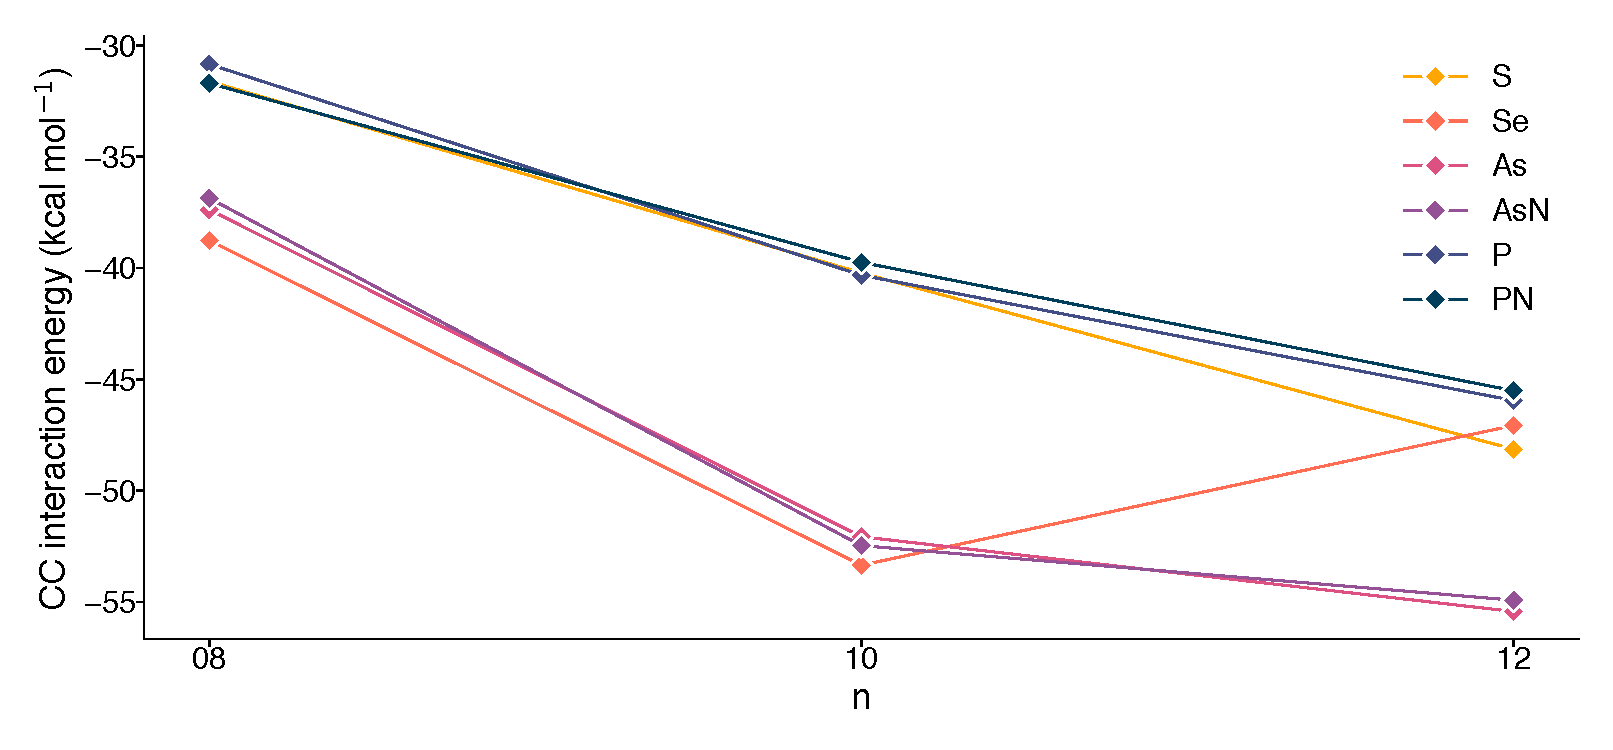
\includegraphics{counterpoise-energies}
    \caption[Counterpoise corrected interaction energies]{Counterpoise corrected interaction energies as weighted averages for all of the sets}
    \labfig{counterpoise-energies}
\end{figure}

As it can be noted, all of the systems present negative interaction energies, that is, the complex has a lower energy than the sum of the energies of its constituents.
This is a good indication that the systems are all stable and can be further studied.
All of the families (except for Se) appear to have a common tendency: the higher the amount of petals, the higher the stabilization. This could be due to the flower having a larger area and bending in a way that maximizes the interactions with the STX molecule.

\section{Study of UV-vis behavior}
\labsec{complex-uv}
One of the main points of adsorbing the STX to the flowers is the desire of increasing its range of absorption of UV-vis radiation.
It's possible that the flower-STX complex absorbs light at longer wavelengths than the isolated STX, and this could be highly beneficial to apply further detection techniques based on resonace.

\subsection{General UV-vis spectroscopy}
Electronic spectra were calculated as described in \refsec{electronic-transition-study} and \refsec{spectra-envelope-calculation} for the most stable conformers of all of the flower-STX complexes.

First, they were plotted together with the UV-vis spectrum of STX and of their corresponding isolated flower.
The individual transitions with significant weights were also plotted as straight vertical lines.
This allowed us to compare the absorption ranges of the complex versus those of the isolated STX and flowers, and to judge if the shifting effect is good enough.

As an example of this, the UV-vis spectra of STX, S08 and S08-STX are displayed in \reffig{uv-s08}.

\begin{figure}
    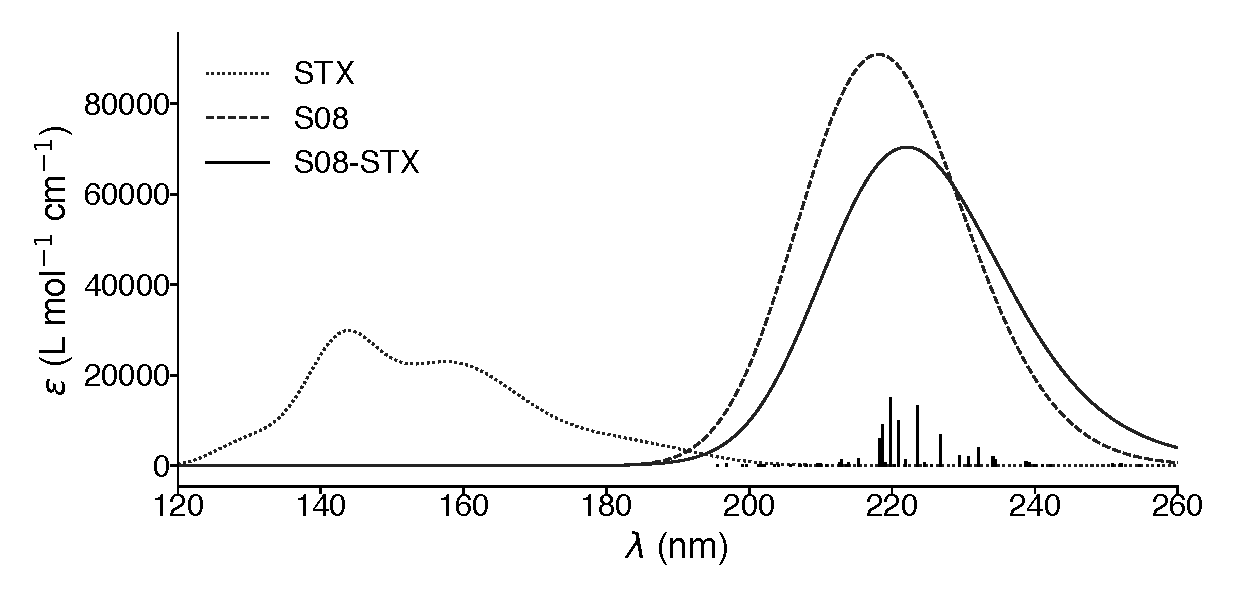
\includegraphics{uv-s08}
    \caption[UV-vis spectrum of S08-STX]{UV-vis spectra of S08-STX and its components}
    \labfig{uv-s08}
\end{figure}

As it may be noted, the spectra of the complex has almost the same absorption range as that of the isolated S08, and in any case, it's definitely shifted towards longer wavelengths in contrast with that of STX.
This effect was the same for all of the flower-STX complexes, and the full list of compared UV-vis spectra can be found in \refsec{ap:uv-vis-flowers}.

After this, the UV-vis absorption spectra of all of the complexes were plotted together in order to visually compare just their absorption ranges. This plot is displayed in \reffig{complex-uv}, where the main heteroatoms of the flowers and their number of petals are distinguished using different colors and linestyles, respectively.

\begin{figure*}
    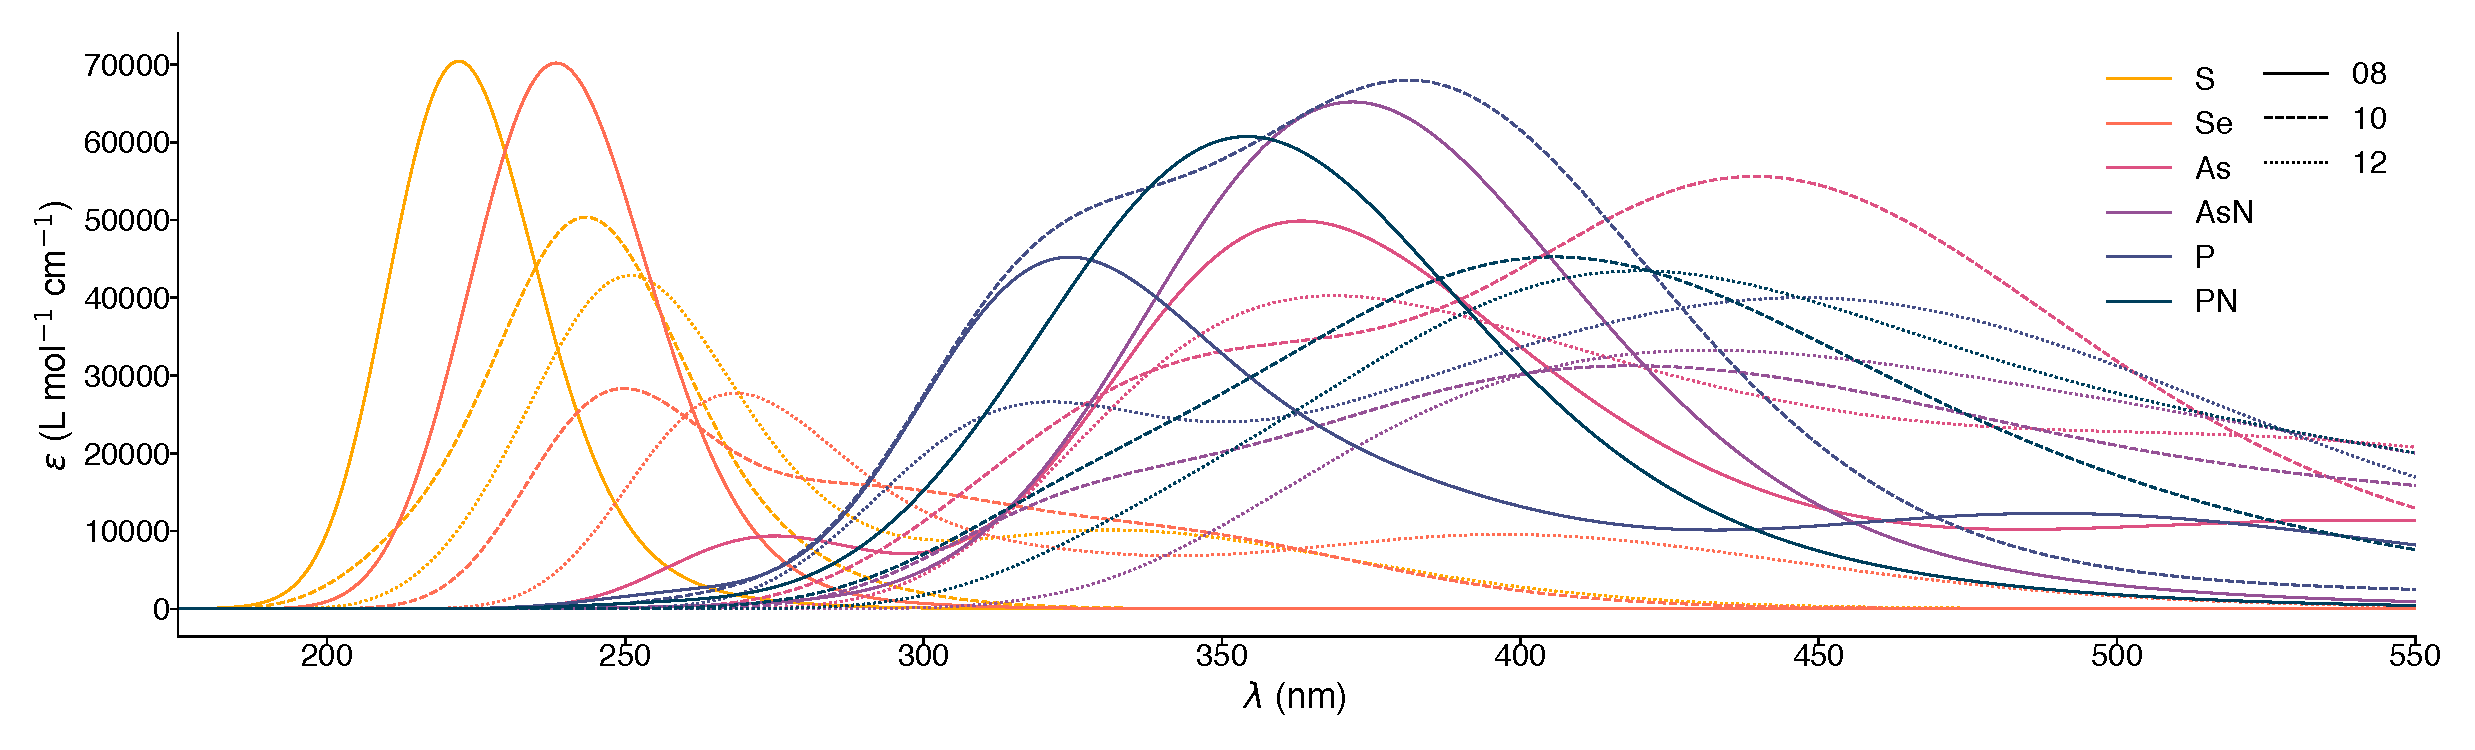
\includegraphics{complex-uv}
    \caption[UV-vis absorption spectra of all complexes]{UV-vis absorption spectra of all flower-STX complexes}
    \labfig{complex-uv}
\end{figure*}

Since this work aims to propose realistic detection techniques, it's important that the systems are actually detectable and identifiable in a real setting.
With this purpose in mind, and keeping into account the usual wavelengths of commercially available lasers for Raman,\sidenote{Which, as detailed in \refsec{previous-work}, lie between \SI{244}{\nano\metre} and \SI{1064}{\nano\metre}} all of the complexes with absorption ranges starting below \SI{250}{\nano\metre} were filtered out.
From the remaining ones, a select few were hand-picked according to the upper limit of their ranges and to their specific individual electronic transitions.
This left us with 8 systems out of the starting 18, which were deemed as a sufficient amount to continue with the last part of the study.

\begin{margintable}
    \centering
    \caption[UV absorption range of selected complexes]{UV absorption range of selected complexes}
    \begin{tabular}{@{}rc@{}}
        \toprule
        System & $\lambda$ (\si{\nano\metre}) \\
        \midrule
        As10 & 300-600 \\
        As12 & 300-900 \\
        AsN08 & 300-450 \\
        AsN10 & 300-650 \\
        AsN12 & 350-850 \\
        P12 & 300-700 \\
        PN10 & 300-550 \\
        PN12 & 325-625 \\
    \end{tabular}
    \labtab{uv-ranges}
\end{margintable}

The UV absorption range for those remaining complexes was also displayed on \reftab{uv-ranges} for convenience.

\section{Resonance Raman}
At last, it was time to apply the previous parts of the study and test the performance of the selected sunflowers.
As seen in \refsec{complex-uv}, all of these complexes have absorption ranges that could be useful in real life, and all of them should be able to be subject the resonance Raman phenomenon.
The main point of this section is generating actual amplified Raman spectra, identifying the lasers that would produce the best amplifications, and being able to select a flower that makes the identification of STX easier.

\subsection{Generation and comparison of spectra}
\labsec{heatmaps}
RR spectra were generated for each of the flower-STX systems by using incident laser wavelengths in their particular ranges of absorption.
Specifically, the whole of their absorption interval was covered by selecting wavelengths with a step of \SI{3}{\nano\metre}.\sidenote{So in the case of As10, for example, the Resonance raman calculations were performed with lasers of \num{300}, \num{303}, \num{306}... all up until \SI{600}{\nano\metre}}

The RR calculations from this step amounted to a total of 2858, where the amplification, position and relevance of each vibrational mode\sidenote{\num{186}, \num{204} or \num{222} depending on the size of the flower} had to be evaluated.
For this purpose, the two following metrics were developed.

\subsubsection{Individual molecule contribution to a complex vibrational mode}
The first of these evaluations was differentiating which vibrational normal modes involve the vibration of the flower, which modes involve the vibration of the STX, and which modes are mixed.
As introduced in \refsec{intmodes-methods}, this was done by analyzing the displacements of the vibrations translated into redundant internal coordinates.
To understand how this is done, we will use the As12-STX system as an example.
The standard Gaussian09 output describes normal modes as cartesian displacements of normal coordinates, indicating vectors for each atom.
For instance, the beginning of the output of vibrational normal mode number 42 looks like this:

\begin{lstlisting}[label=normal-mode-output, style=kaolstplain]
                    42
                     A
Frequencies --    229.2846
Red. masses --     36.2305
Frc consts  --      1.1222
IR Inten    --      3.9161
Atom  AN      X      Y      Z
   1  33    -0.15  -0.08   0.01
   2  33    -0.03  -0.04  -0.04
   3   6     0.13   0.06   0.06
   4   6     0.06   0.05   0.01
   5  33     0.10  -0.01  -0.03
               ...
\end{lstlisting}

This contains all of the necessary information to study the movements of the atoms and understand the vibrations of the mode, but it's difficult to interpret.
By specifying the keyword \code{intmodes} in the frequency calculation, this output gets translated into the much more readable redundant internal coordinates notation.
This is As12-STX's mode number 42 in this new format.

\begin{lstlisting}[label=intmodes-output, style=kaolstplain]
              ----------------------------
              ! Normal Mode    42        !
--------------                            --------------
! Name  Definition       Value     Relative Weight (%) !
--------------------------------------------------------
! R1    R(1,34)         -0.0693             0.4        !
! R9    R(4,63)         -0.067              0.4        !
! R15   R(8,9)           0.1332             0.8        !
! A4    A(2,3,30)       -0.0755             0.4        !
! A19   A(10,7,63)       0.0567             0.3        !
! A21   A(5,9,8)         0.1548             0.9        !
! D1    D(36,1,34,24)    0.0965             0.5        !
! D3    D(34,1,36,27)    0.1767             1.0        !
! D5    D(6,2,3,4)      -0.0882             0.5        !
                          ...
\end{lstlisting}

\begin{margintable}
    \centering
    \caption[Classification of individual vibrations]{Classification of the individual vibrations of normal mode 42 for As12-STX (atoms of the flower and the STX are marked in blue and red, respectively)}
    \begin{tabular}{@{}ll@{}}
        \toprule
        Vib. def. &  Category \\
        \midrule
        R(\stx{1},\stx{34})                     & STX \\
        R(\stx{4},\flower{63})                  & Mixed \\
        R(\stx{8},\stx{9})                      & STX \\
        A(\stx{2},\stx{3},\stx{30})             & STX \\
        A(\stx{10},\stx{7},\flower{63})         & Mixed \\
        A(\stx{5},\stx{9},\stx{8})              & STX \\
        D(\stx{36},\stx{1},\stx{34},\stx{24})   & STX \\
        D(\stx{34},\stx{1},\stx{36},\stx{27})   & STX \\
        D(\stx{6},\stx{2},\stx{3},\stx{4})      & STX \\
    \end{tabular}
    \labtab{intmodes-classification}
\end{margintable}

Here the displacements are expressed as bond length extensions between two atoms (R), angle openings and closings between three (A), and dihedral angle torsions between four (D).
Their magnitude is expressed as a single positive or negative value, whose absolute value is then weighted and displayed as the Relative Weight as a percent.
By differentiating whether the atoms involved in a certain vibrational motion belong to the As12 flower or to the STX, said vibration can be classified as an exclusive flower vibration, as an exclusive STX vibration, or as a mixed one.
Such classification, illustrated in \reftab{intmodes-classification}, can be easily automated using a script.

By adding up the relative weights of the vibrations in each category, we can find out which of the elements of the sunflower-STX complex dominate a particular mode.
In this case, mode 42 has a \SI{92.54}{\percent} contribution from the STX, a \SI{0.00}{\percent} contribution from the flower, and a \SI{7.45}{\percent} contribution from mixed vibrations.

From a practical point of view, the fact that it's composed almost exclusively of isolated STX vibrations makes this a good choice of vibrational mode to look for in a RR spectra of this complex.
In contrast to other mixed or flower-exclusive vibrational modes, a mode like this is a clear sign of the presence of the STX.

\subsubsection{Resonance Raman enhancement factor}
Even if a mode is exclusive to our molecule of interest, it needs to have a sufficient intensity in the final spectrum: otherwise it cannot be detected and cannot be of any use in the identification.
In the context of RR, this means that it has to benefit from a certain level of amplification during resonance experiments.

To evaluate this for all of the tested laser wavelengths, the enhancement factor (EF) metric was designed and applied.
The EF for a certain vibrational mode $i$ and laser wavelength $\lambda$ is defined in \refeq{enhancement-factor}.

\begin{equation}
    \labeq{enhancement-factor}
    EF_{i,\lambda} = \log_{10}\left(\frac{I_{i,\lambda}}{I_{i,\textit{SL}}}\right)
\end{equation}

In this equation, $I_{i,\lambda}$ corresponds to the Raman activity of the mode $i$ in the amplified spectrum, and $I_{i,\textit{SL}}$ is the activity of the same mode in a regular Raman prediction.
Using a logarithmic scale makes easier to visualize the very high amplifications that arise with this technique, which in the case of this work, have reached values near \num{10e10} times than the standard Raman.

Similarly as before, this calculation is easy to automate and can serve as a way to filter out wavelengths that don't generate sufficient amplification, or discard modes that aren't sufficiently amplified.

\subsubsection{Combined resonance graphs}
In order to make use of the two newly defined metrics, an output file processing pipeline was designed.
Large amounts of data from the internal mode decompositions, standard Raman spectra and many amplified RR spectra were processed, combined and analyzed using Python scripts.

This information was filtered and displayed in the following manner:
First, Gaussian envelopes for all of the RR spectra as well as the standard Raman spectrum were calculated.
These envelopes were equivalent to those used in previous Raman spectra: \num{10000} points divided across the most relevant range for each system.
Then, each of the points in the amplified RR curves was converted into EF values using \refeq{enhancement-factor}.
These were plotted as a colored grid: all of the RR wavelengths on the vertical axis, and the \num{10000} calculated wave number values on the horizontal axis.
The squares of the grid, therefore, were colored according to the calculated EF values.

This resulted in quite colorful graphs where the brightest horizontal lines correspond to the laser wavelengths that generate the largest amplifications, and bright vertical areas correspond to highly amplified vibrational modes.

Then, in order to make full use of the metrics, these graphs were annotated using a special procedure.
In regard to the vibrational modes, two thresholds were set: a maximum percent of flower contribution, and a minimum percent of STX contribution.
This ensured that the displayed modes were relevant.
As for the laser wavelengths, only the ones that produced amplifications above a certain threshold value for the EF of the previously selected vibrational modes were displayed.

It should be noted that the values of these metrics varied very significantly between the different systems.
Therefore, setting common thresholds for all of them was unpractical: the values that worked for a certain complex were too strict for others.
For this reason, the thresholds were set individually for each of the systems in a such a way that only the top 5, 6 or 7 lasers and the best 5, 6 or 7 vibrational modes were selected and labeled.
The cutoff values for these top results, therefore, were annotated in each of the graphs.

Applying this method to the running example of AsN12-STX, then, resulted in \reffig{comb-asn12}

\begin{figure}
    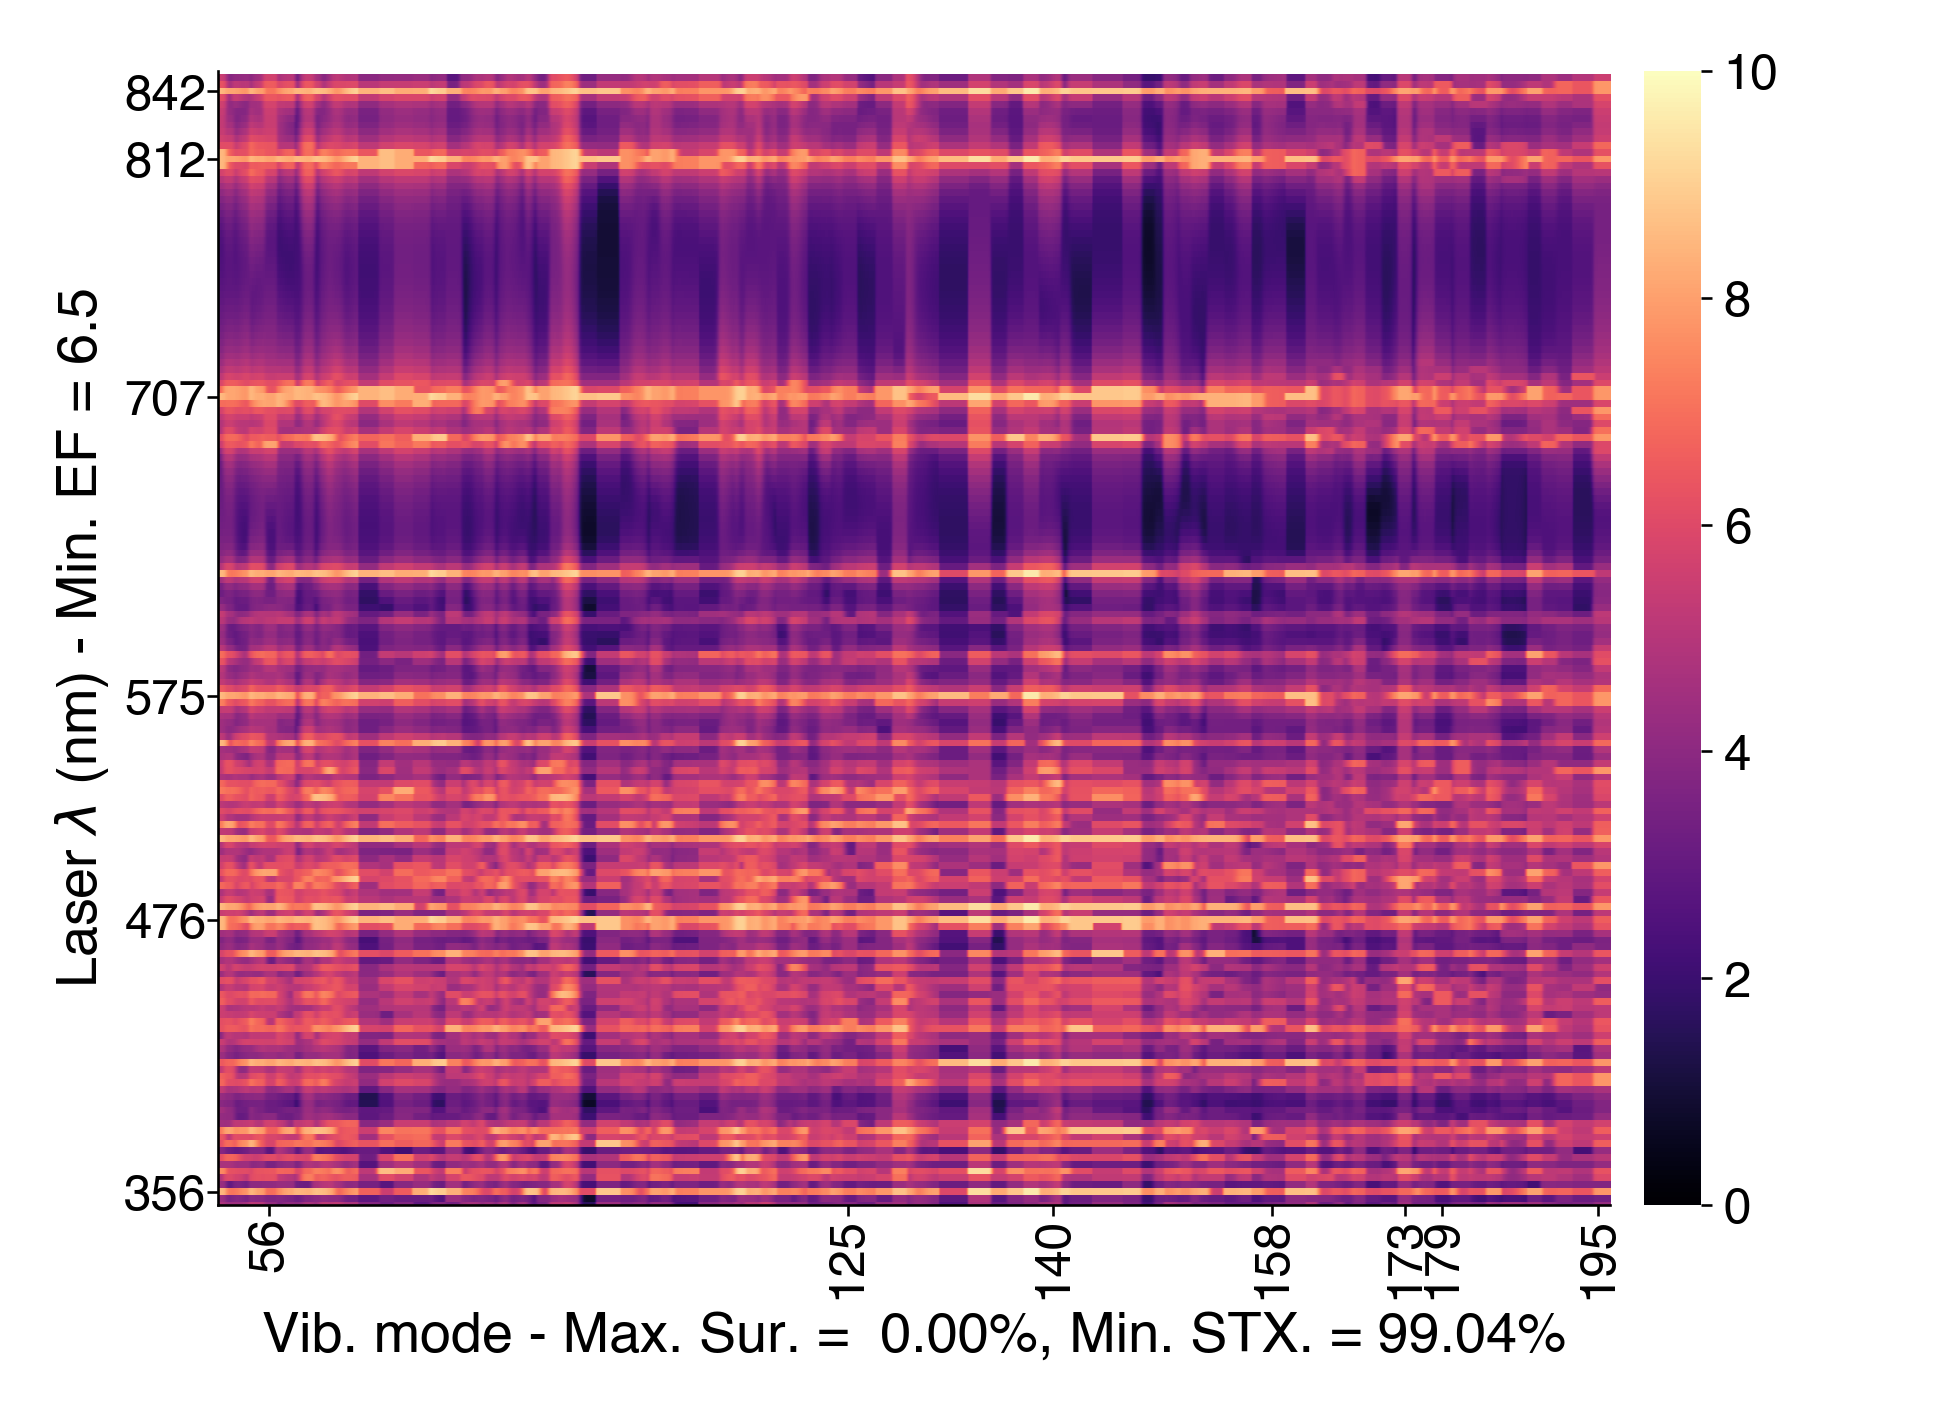
\includegraphics{comb-asn12}
    \caption[Combined resonance graph for AsN12-STX]{Combined resonance graph for AsN12-STX}
    \labfig{comb-asn12}
\end{figure}

\begin{margintable}
    \centering
    \caption[Electronic transitions of AsN12-STX]{Major electronic transitions of AsN12-STX}
    \begin{tabular}{@{}S[table-format=3.1]
                       S[table-format=1.4]@{}}
        \toprule
        {$\lambda$ (\si{\nano\metre})} & {f (a.u.)} \\
        \midrule
        366.8 & 0.0746 \\
        375.0 & 0.0986 \\
        407.7 & 0.1021 \\
        548.3 & 0.1972 \\
        599.8 & 0.0117 \\
        638.6 & 0.0052 \\
        794.27 & 0.0089 \\
    \end{tabular}
    \labtab{asn12-transitions}
\end{margintable}

As it can be observed, the laser wavelengths with the highest amplifications can be clearly distinguished at a glance as bright yellow horizontal lines.
Comparing these wavelengths to those of the major electronic transitions found in the UV-vis spectra, most of them are found matching.
The UV-vis spectrum of ANs12-STX and some of its most relevant transitions have been included in \reffig{uv-asn12} and \reftab{asn12-transitions}.
This confirms that the amplification effect is related to the molecule reaching excited electronic states, supporting the theory behind resonance Raman.
While many of the bright horizontal lines of the graph don't have a label, they have great enhancement factors nonetheless; they just weren't marked because the amplification of the selected modes were not particularly high in comparison with the amplification of other less relevant ones.

\begin{figure}
    \includegraphics{uv-asn12}
    \caption[UV-vis spectrum of AsN12-STX]{UV-vis spectrum of AsN12-STX, with its 50 major transitions plotted as vertical lines}
    \labfig{uv-asn12}
\end{figure}

The main reasonings behind this interpretation are valid for the rest of the combined EF graphs, which can be found in \refsec{ap:combined-ef}, and it's possible to quickly visually identify the best laser wavelengths and vibrational modes for all of them.
However, it was also possible to see that one of them presented better properties than others.

\begin{figure}
    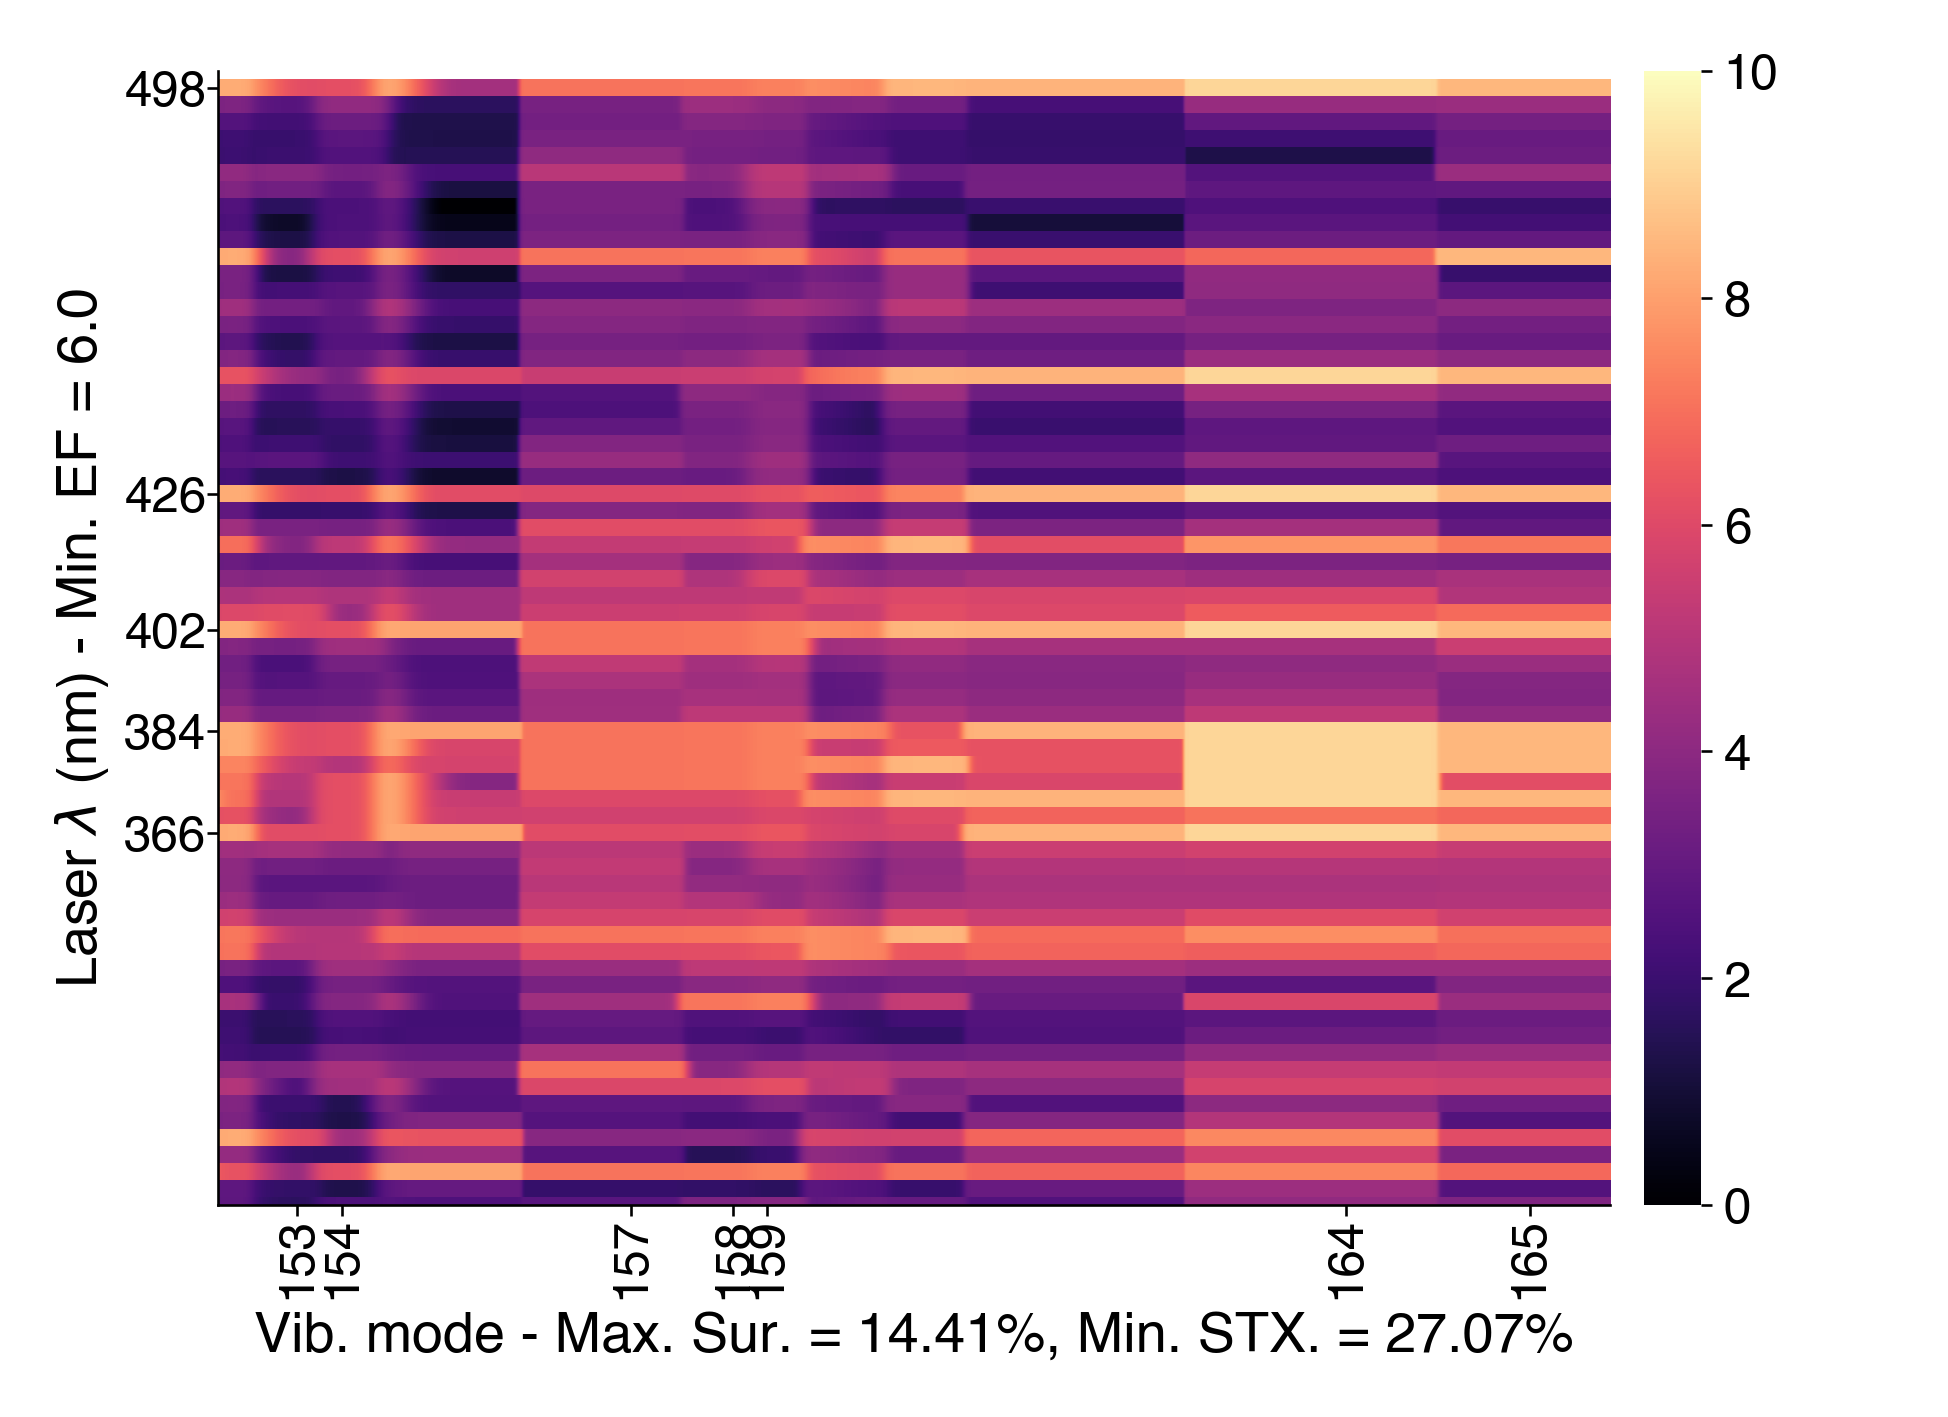
\includegraphics{comb-asn08}
    \caption[Combined resonance graph for AsN08-STX]{Combined resonance graph for AsN08-STX}
    \labfig{comb-asn08}
\end{figure}

Let's take the AsN08-STX system.
Its combined graph is similar to that of AsN12-STX in the sense that it's easy to interpret and it has a similar number of labels.
However, looking at the cutoff values, it can be observed that the ones for AsN08-STX are lower.
For example, the cutoff value for the EF in the AsN08-STX system is \num{6.0}, while in the AsN12-STX system it's \num{6.5}.
From a vibrational mode composition point of view, AsN08-STX's most pure vibrations were only guaranteed to have more than \SI{27.07}{\percent} STX contribution; while for AsN12-STX the labeled modes had over \SI{99.04}{\percent}.
It appeared that the flowers with a higher number of petals allowed for greater amplifications and more pure vibrational modes.
The exception to this tendency was PN12-STX, which had vibrational modes much less pure than the rest of 12-petal systems.

\subsection{Final selection}
While the previous method serves as a convenient way to visualize the best amplifications, it's true that it deviates a little from the usual representations of Raman data.
This final section aims to tie this insight together, and to display it in a more standard way in order to facilitate the comparison and selection of a definitive combination of flower, laser wavelength, and set of vibrational modes.

For this reason, a complementary way of plotting amplified Raman spectra was designed: drawing the amplified RR spectra of all of the previously selected laser wavelengths vertically sorted in a single plot.
The graphs in this section don't include any units of intensity: the reason for choosing these wavelengths, precisely, was that they had high enough amplifications.

\begin{figure*}[h]
    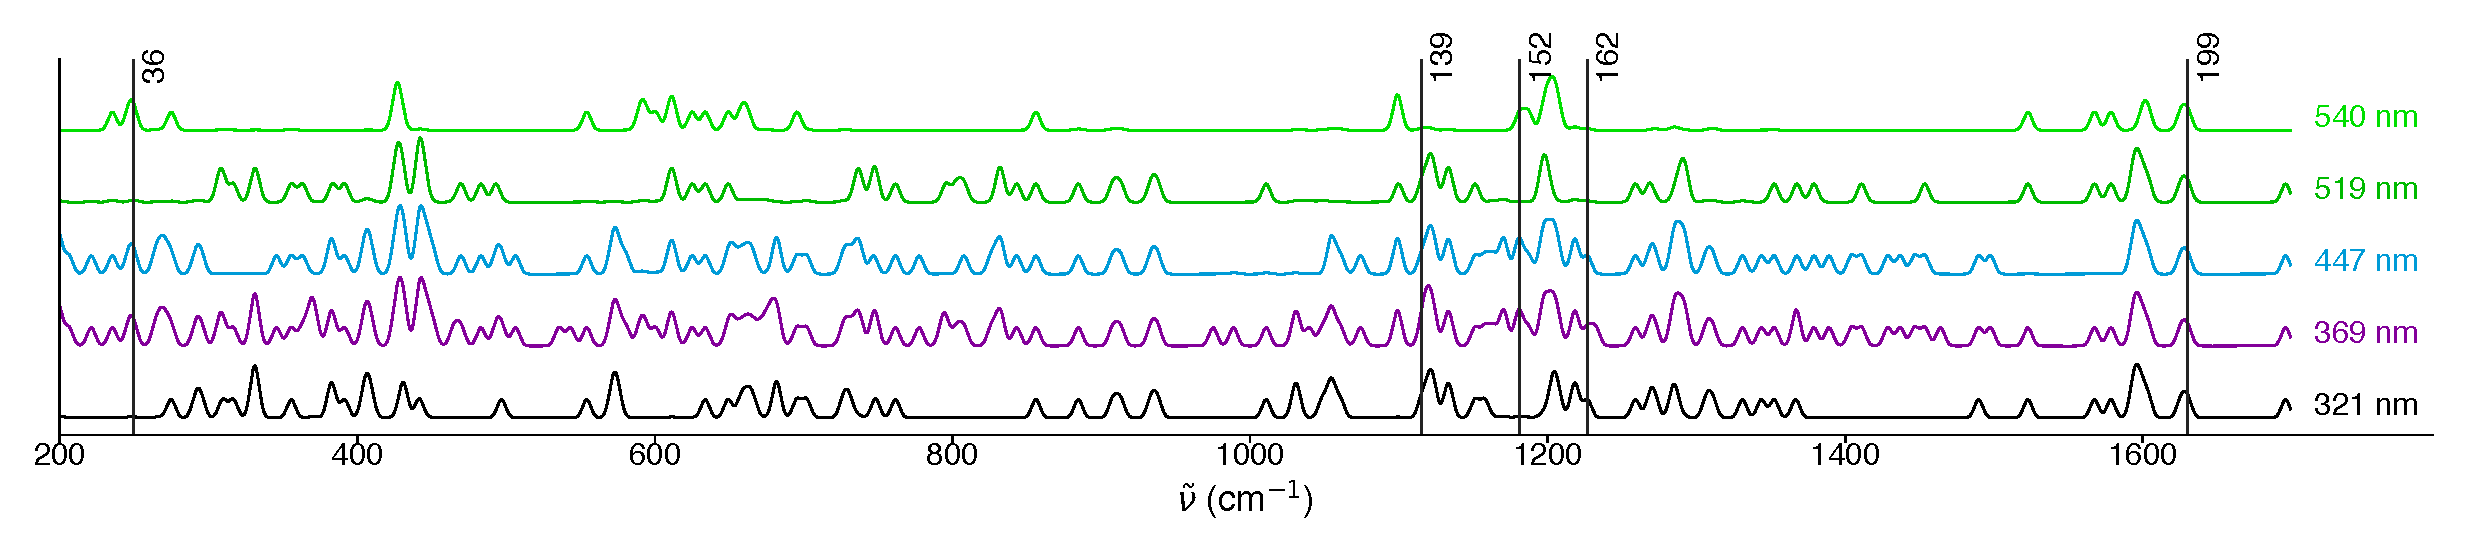
\includegraphics{unfolded-p12}
    \caption[short]{long}
    \labfig{body:unfolded-p12}
\end{figure*}

Taking the P12-STX system as an example due to its clarity, the RR spectra for its selected wavelengths were plotted and displayed in \reffig{body:unfolded-p12}.
Using this type of graph, one can easily compare which modes have the best amplifications at each of the considered wavelengths.
In this case, it can be observed that mode 36 is only visible at \SI{369}{\nano\metre}, \SI{447}{\nano\metre} and \SI{540}{\nano\metre}.
Mode 139 can be detected with all of the laser wavelengths except for \SI{540}{\nano\metre}.
However, mode 162 is only active at \SI{321}{\nano\metre}, \SI{369}{\nano\metre} and \SI{447}{\nano\metre}.
Following this kind of logic, it's possible to select the wavelength that maximizes the number of relevant vibrational modes that are visible.
This set of vibrational modes and this laser wavelength, then, would be the ones that could be used in an analytical setting to detect and quantify the presence of STX in a sample.
In the case of P12-STX, then, the chosen wavelengths could be \SI{369}{\nano\meter} or \SI{447}{\nano\meter}, given that all of the chosen vibrational modes (\num{36}, \num{139}, \num{152}, \num{162} and \num{199}) are visible in their amplified spectra.

All of the RR spectra for the rest of the flower-STX systems can be found in \refsec{ap:rr} along the corresponding commentary.

As a way of clearly displaying these final results and selection, a last way of plotting the Raman data of a single incident laser wavelength was devised.
This one, in addition to displaying the main Raman spectrum and the labels of the main vibrational modes, also included a representation of its numerically calculated derivative.
This type of representation was applied to the P12-STX system using the previously chosen \SI{447}{\nano\meter} incident laser wavelength, and displayed in \reffig{body:final-p12}.

\begin{figure*}[h]
    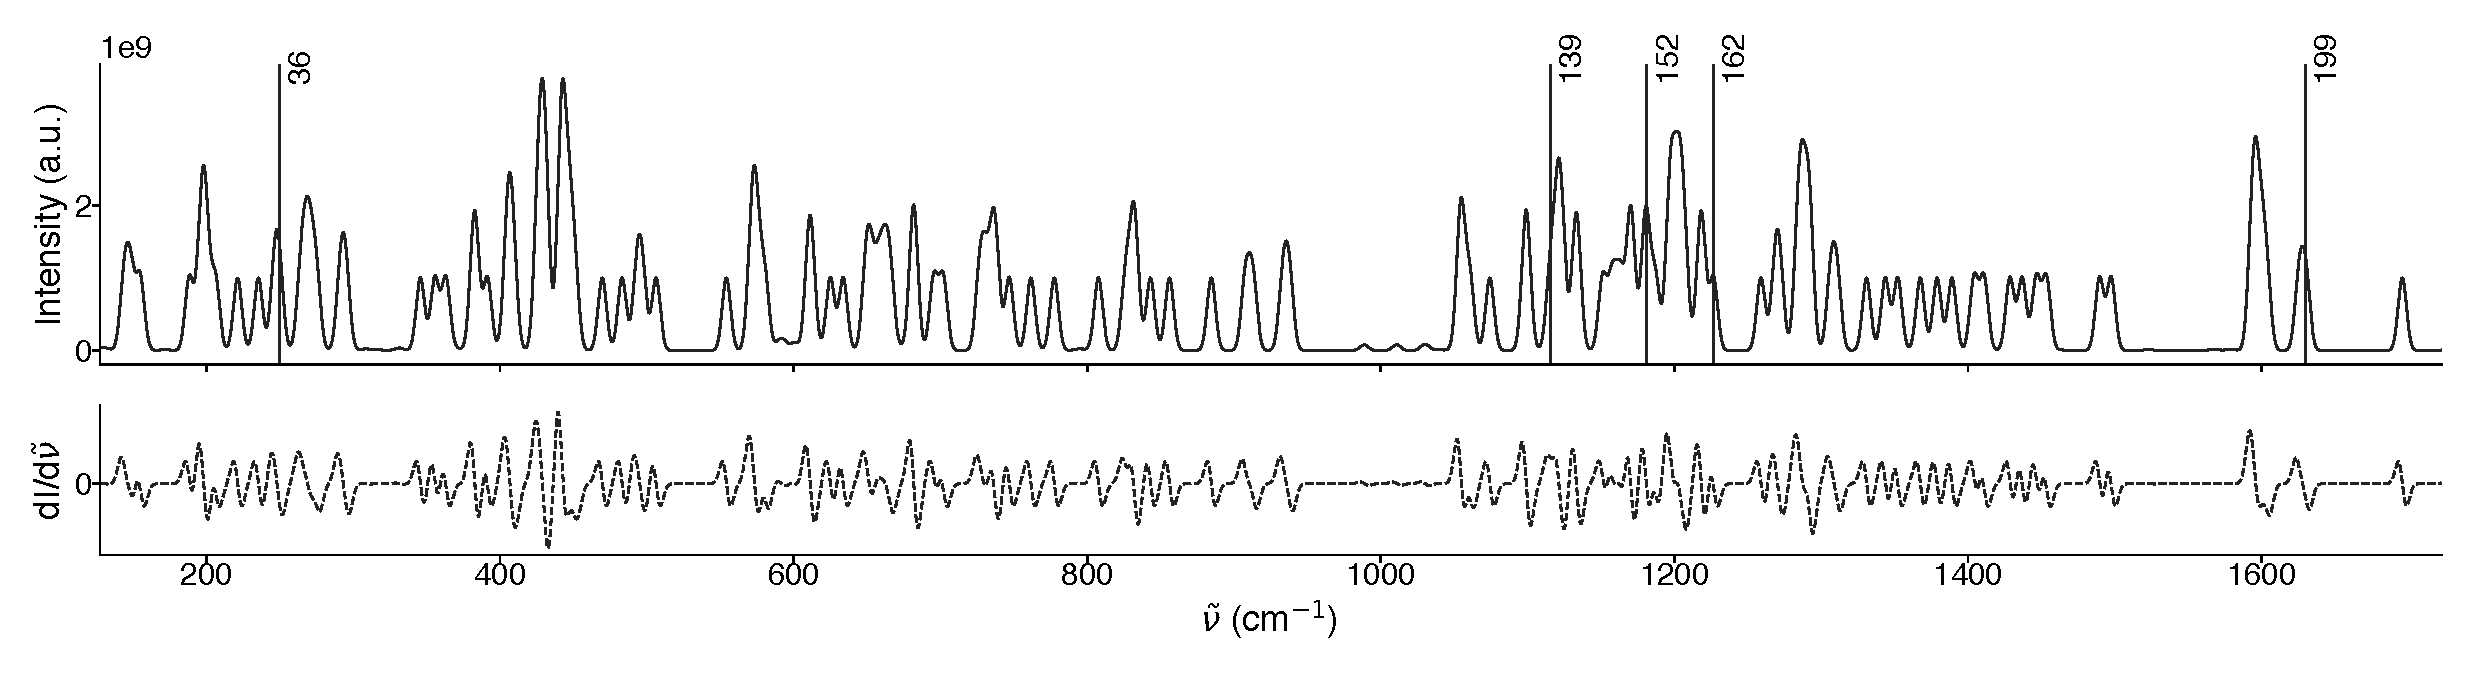
\includegraphics{final-p12}
    \caption[short]{long}
    \labfig{body:final-p12}
\end{figure*}

As it can be observed, the selected vibrational modes are clearly distinguishable, and the shape of the Raman peaks is more clear as there's only one line.
At the chosen incident laser wavelength, they are all highly amplified (in the order of \num{1e9} a.u., with EF values higher than \num{5.4}).
The addition of the derivative makes it easier to locate the peaks and evaluate their cleanliness.


\section{Conclusions}

Again, listing the most important points of this chapter as a form of conclusion:

\begin{itemize}
    \item STX+2 was previously found to be the only protonated species present at the gentle pH of 6 (in contrast with higher pH values, where multiple protonated species coexisted), so the whole study was carried out using this structure.
    \item STX's vibrational spectroscopic profile was described by studying its Raman spectrum and selecting its key vibrations
    \item The electronic spectroscopy of STX was studied by generating its UV-vis spectrum.
    \item STX's UV-vis absorption range, from \SI{120}{\nano\metre} to \SI{200}{\nano\metre}, was considered too low in the spectrum of light to apply resonance Raman amplification in a real life setting. This was the main motivation behind the application of sunflowers as substrates
    \item It was found that there were stable conformations for all of the flower-STX complexes. The importance of these conformers was evaluated using Maxwell-Boltzmann statistics.
    \item Their corrected interaction energy was calculated using the Counterpoise method, and it was found that larger flowers tended to form more stable complexes.
    \item The UV-vis spectra for all of the flower-STX complexes were generated and compared to those of the isolated flowers and STX. It was observed that in all cases the absorption ranges were greatly shifted towards larger wavelengths, but only 8 of the 18 flowers were selected to continue with the study due to their better properties.
    \item A method to quantitatively evaluate the contributions of each of the molecules of a complex to a its compound vibrational modes was developed. It was applied to the flower-STX complexes in order to select the modes with the highest STX contributions.
    \item The enhancement factor, a metric to evaluate the amplifications caused by a laser of a certain wavelength in a RR setting, was defined. It was applied to the flower-STX complexes to select the best lasers based on how much they amplified the intensity of the previously chosen vibrational modes.
    \item A final selection of normal vibrational modes and laser wavelengths was done for each of the 8 flower-STX complexes, and it was displayed in two different forms.
\end{itemize}

In general, the outcome of this chapter was considered a success.
Many of the proposed sunflowers were considered appropriate for the STX molecule resulting in great amplifications of their key modes, and in the end, realistic combinations of vibrations and lasers were selected for each of them.

\setchapterimage[2cm]{../images/header-conclusions.jpg}
%\setchapterpreamble[u]{\margintoc}
\chapter{Summary and final conclusions}
\labch{conclusions}

All in all, the development and results of the work were considered satisfactory.
Translating the proposals made throughout this work to the real world would be no easy task as it would involve many steps and many different areas of expertise: the design of effective synthetic routes for the sunflowers, the preparation of portable devices that could carry them, the selection of a technique to obtain samples contaminated by STX, the development and tuning of analytical techniques based on the resonance effect...
In any case, all of these challenges could be pointed in the right direction and made easier thanks to this previous computational exploration.

Considering only theory and computation, however, the techniques already discussed in this work could be expanded, improved and continued in many ways, such as the following:

\begin{itemize}
    \item Studying the possibilities of using different methods or larger basis sets. The selected calculation level was considered to be a good fit for the problem at hand considering the number of calculations that needed to be done and the available computational power. However, now that the problem is more mature and well known, some of its parts could be better described by translating them to higher levels of computation
    \item Complementing the description of the aromaticity of the sunflowers using alternative techniques such as the study of the anisotropy of the current induced density\sidenote{Most commonly known as ACID\cite{geuenich17,geuenich17-2}}. Aromaticity is a complex property with many dimensions, and observing it from additional points of view could only improve its understanding
    \item Expanding and packaging the NICS python program so it can easily be distributed and applied to study the NICS profile of any non-planar surface-like part of a molecule
    \item Delving deeper into the nature and composition of the electronic transitions of the flowers, the STX and the flower-STX complexes
    \item In a similar line of research, analyzing the transfers of charge that occur within the complexes when these electronic excitations happen. This could serve as a way to explain the magnitude and nature of the observed resonance effects
    \item Investigating the possible fluorescence effects that could arise in a real life resonance Raman measurement using certain laser wavelengths
    \item Determining the nature of the possible implications of SERS effects in the Raman amplifications
    \item Expanding the study to flowers with other different heteroatoms and/or other numbers of petals
    \item Determining the nature of the flower-STX system's non-covalent interactions
    \item Studying the adsorption of the STX to the flowers in a more realistic setting by adding the simulation of a solvent to the calculations
    \item Simulating the interactions that would occur in a system with many molecules of sunflower and STX
\end{itemize}

As many of these suggestions were well beyond the scope or computational availability of this work, they remain as open lines of research, ready to be expanded upon in the future.
At the moment, however, the level of depth attained in this text in particular was considered sufficient for its objectives as an end of master's theses.

Finally, as a way to close off this little book, a piece of the author's mind on the general purpose of a work like this:
The aim of \refch{sunflowers} was to provide insight into this novel family of sunflowers, but also to illustrate a series of characterization techniques that could be utilized to describe a variety of different surface-like systems.
In a similar way, while STX was the protagonist of \refch{stx} due to the previous studies in which the research group was involved, the flowers could be applied to a number of different toxins or molecules with analytical interest.
The procedures shown and proposed all throughout this work are meant to serve as suggestions and references to similar studies: keeping their purposes, strengths and limitations in mind, they could be made useful in many different contexts; and even serve as starting points in the development of better and more sophisticated methodologies well beyond the scope of the author's reach.


\appendix % From here onwards, chapters are numbered with letters, as is the appendix convention

\pagelayout{wide} % No margins
\addpart{Appendix}
\pagelayout{margin} % Restore margins

\pagelayout{marginap}
\chapter{Additional graphs and spectra}

\newpage
\section{NICS of all sunflowers}
This sections includes the results for the NICS calculations described in \refsec{nics} applied to all of the isolated sunflower molecules.

All of the systems except for the As and P families have magnetic properties that hint towards aromaticity.
As08, P08 and P10 are clearly antiaromatic.
As10 has a less clear profile, but also seems to tend to antiaromaticy.
As12 and P12 are the less clear of them all, but also seem to have an antiaromatic magnetic behavior.

\begin{figure*}[h]
\centering
\begin{subfigure}{5.5cm}\centering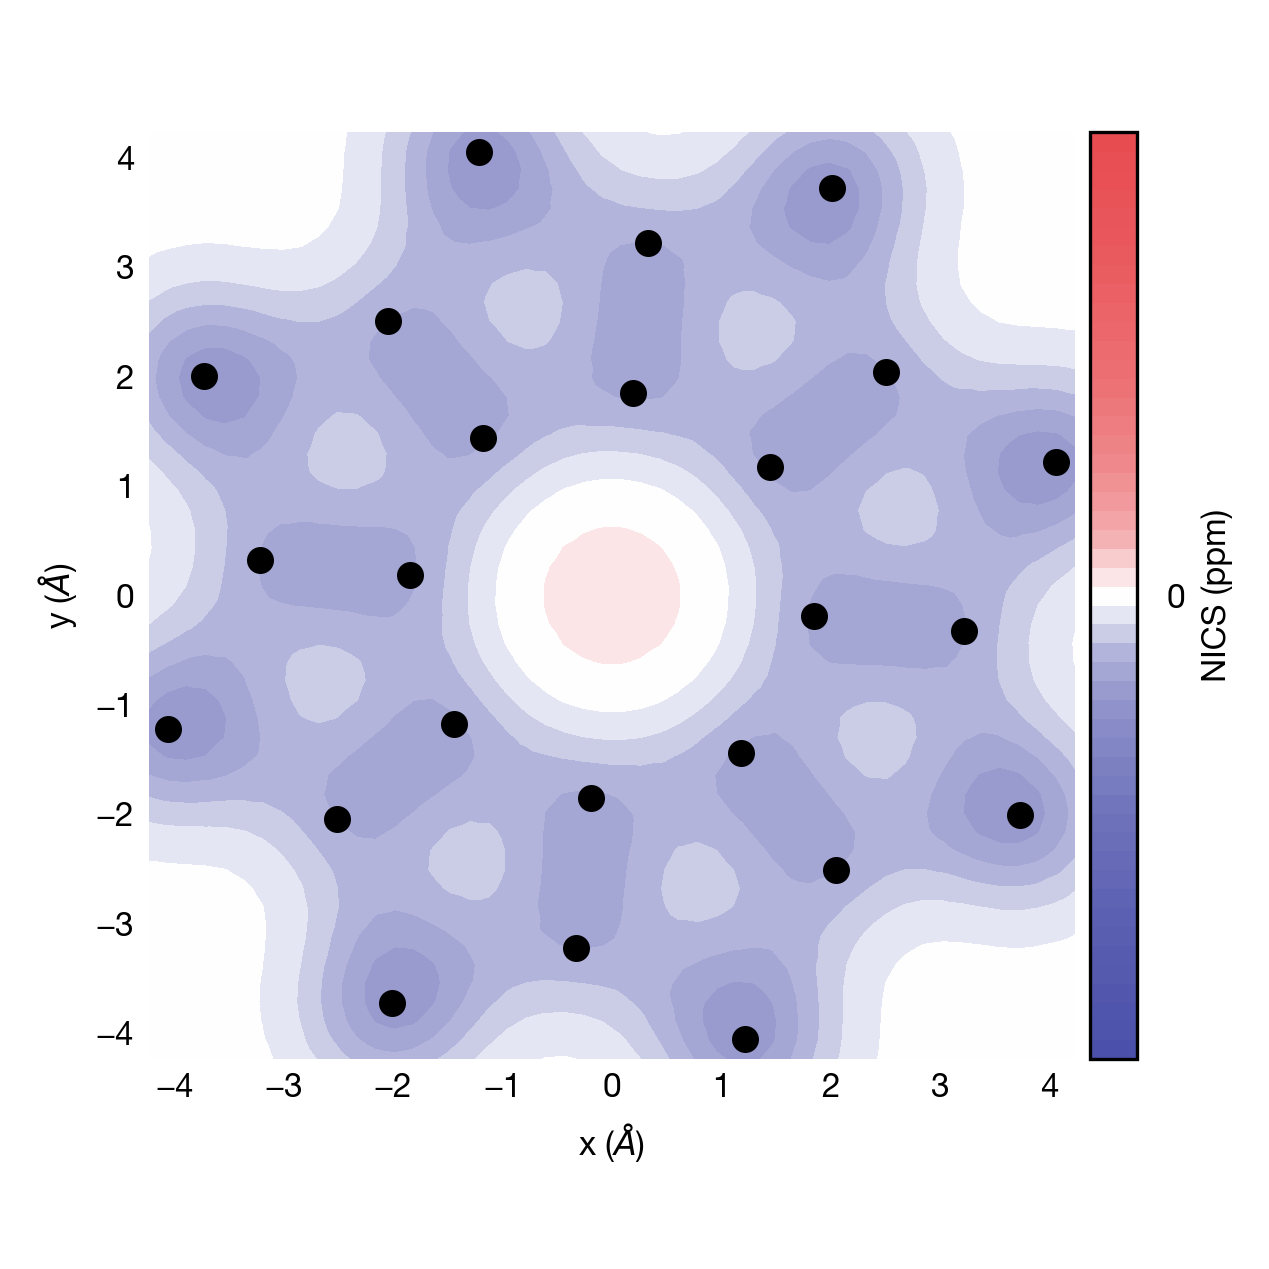
\includegraphics{s08-2d}\caption{NICS 2D projection for S08.\\Aromatic character}\end{subfigure}%
\begin{subfigure}{5.5cm}\centering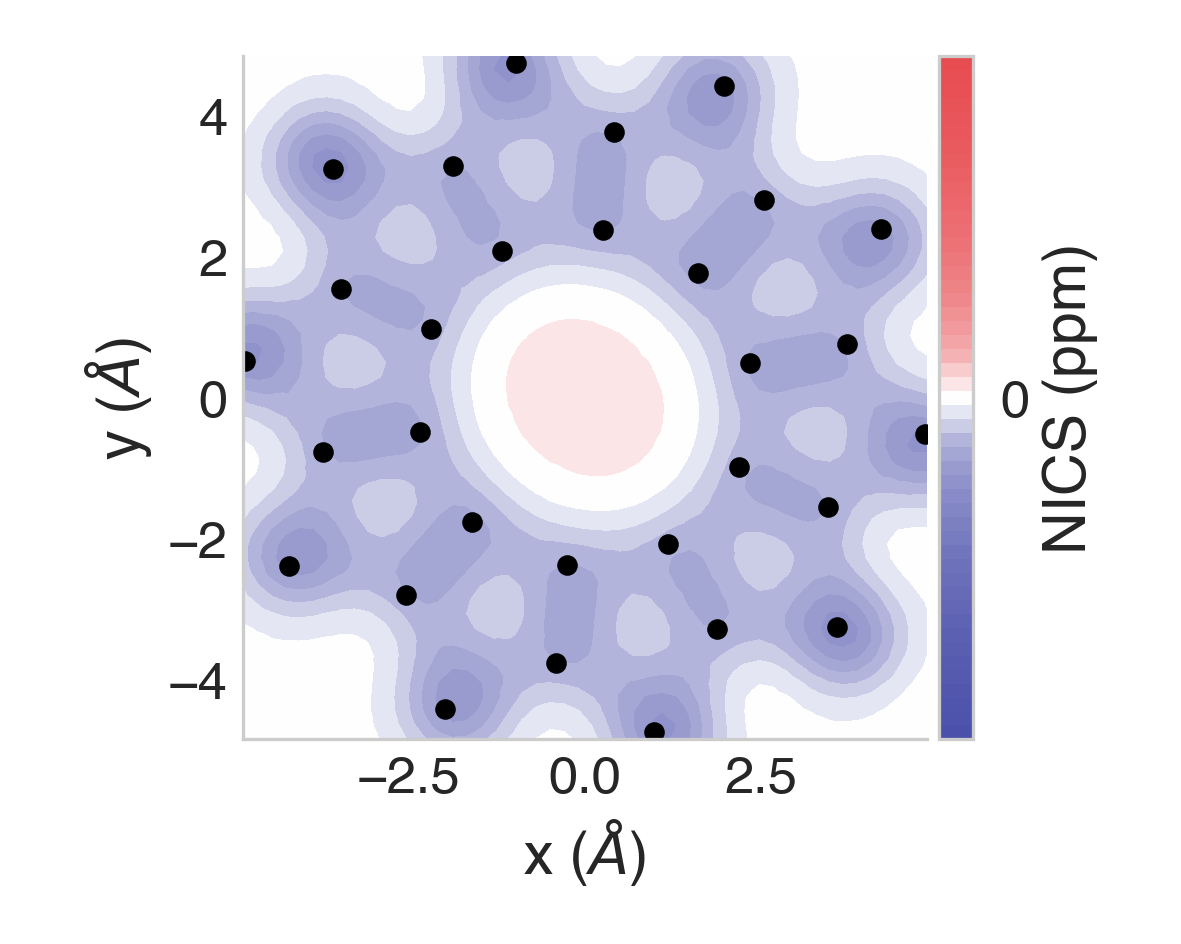
\includegraphics{s10-2d}\caption{NICS 2D projection for S10.\\Aromatic character}\end{subfigure}%
\begin{subfigure}{5.5cm}\centering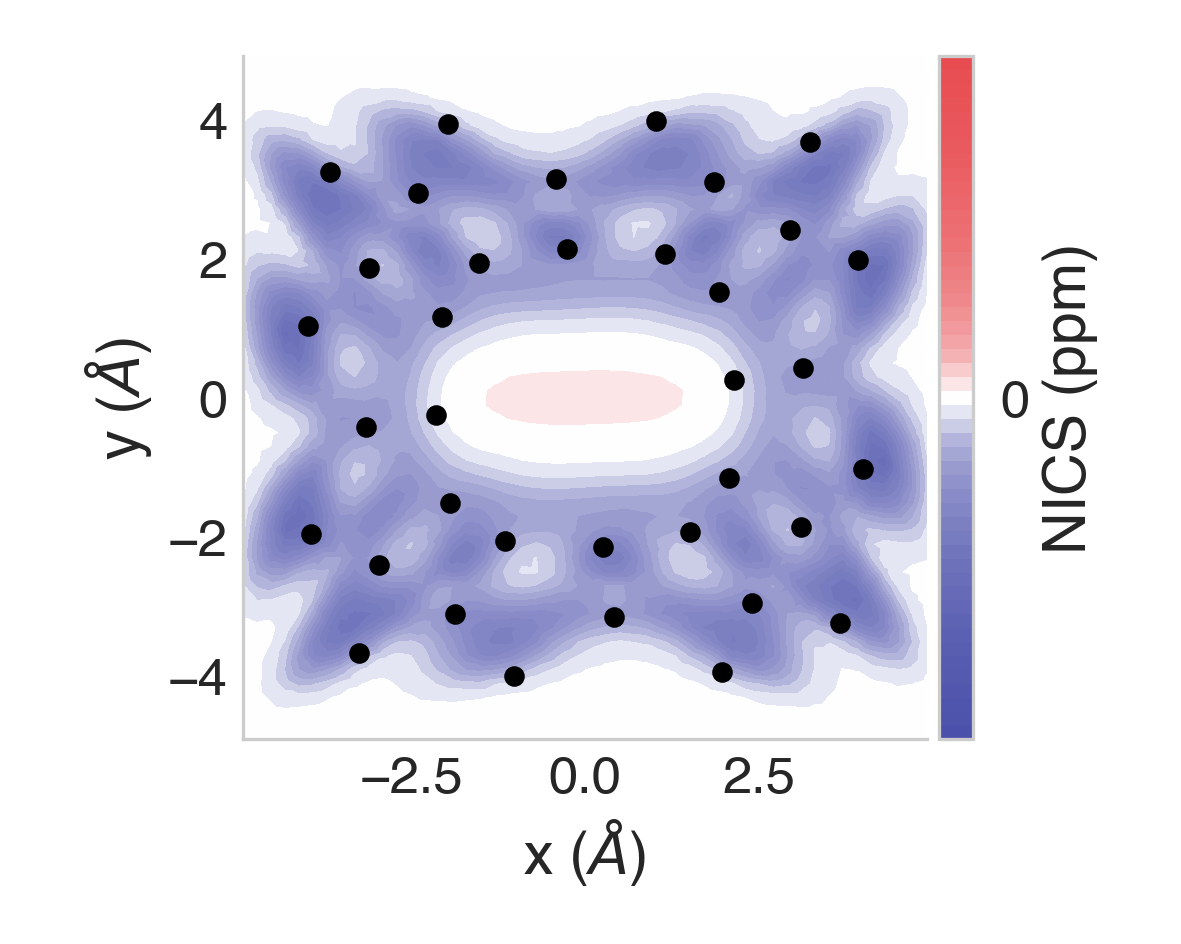
\includegraphics{s12-2d}\caption{NICS 2D projection for S12.\\Aromatic character}\end{subfigure}
\begin{subfigure}{5.5cm}\centering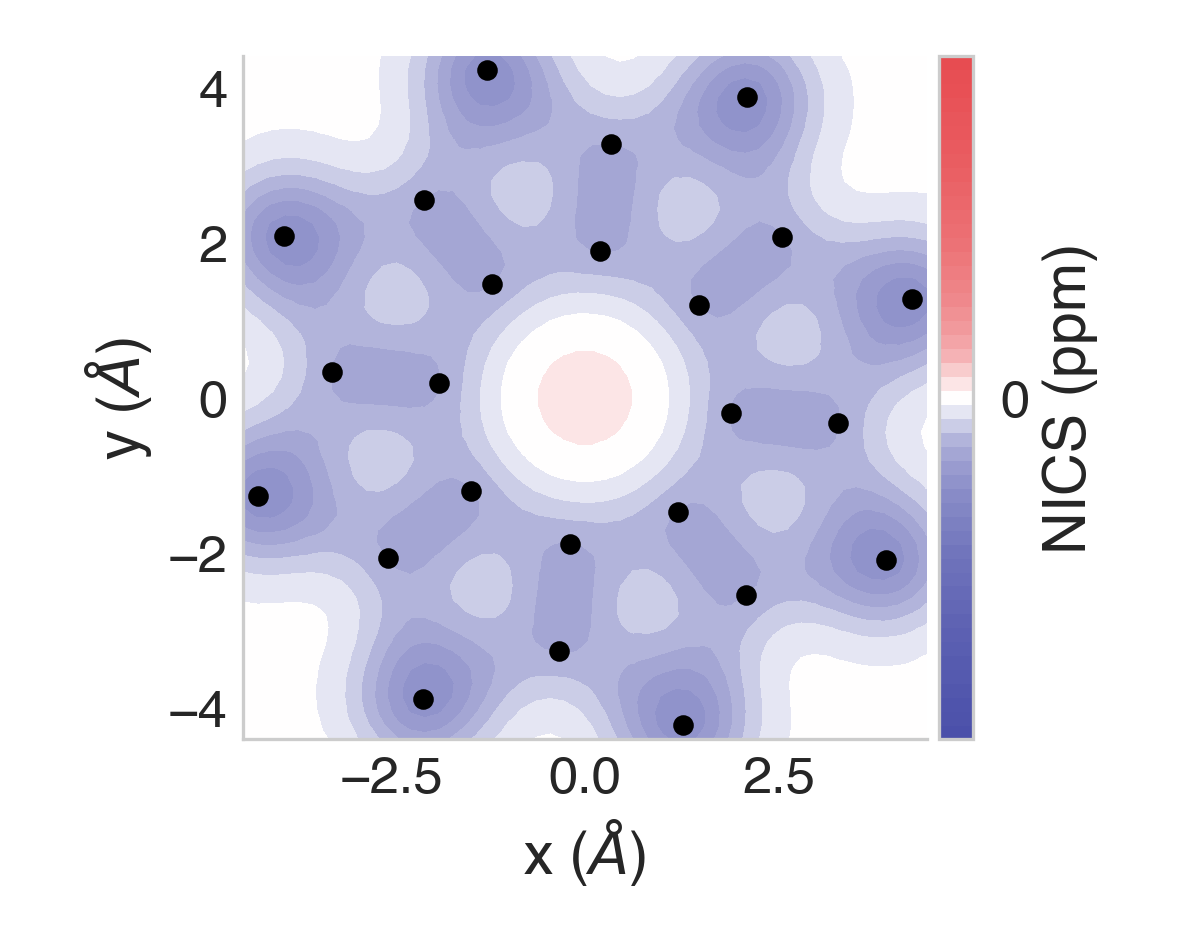
\includegraphics{se08-2d}\caption{NICS 2D projection for Se08.\\Aromatic character}\end{subfigure}%
\begin{subfigure}{5.5cm}\centering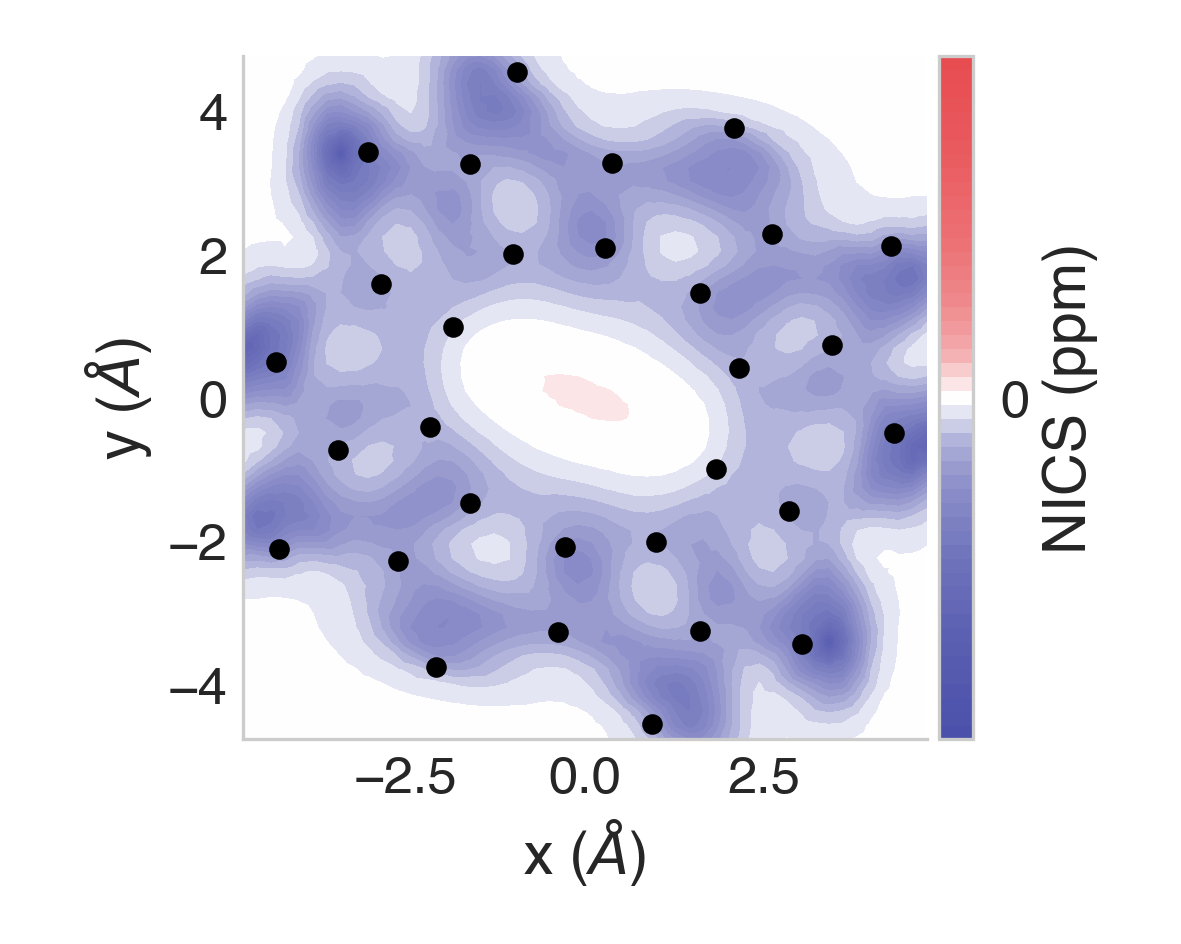
\includegraphics{se10-2d}\caption{NICS 2D projection for Se10.\\Aromatic character}\end{subfigure}%
\begin{subfigure}{5.5cm}\centering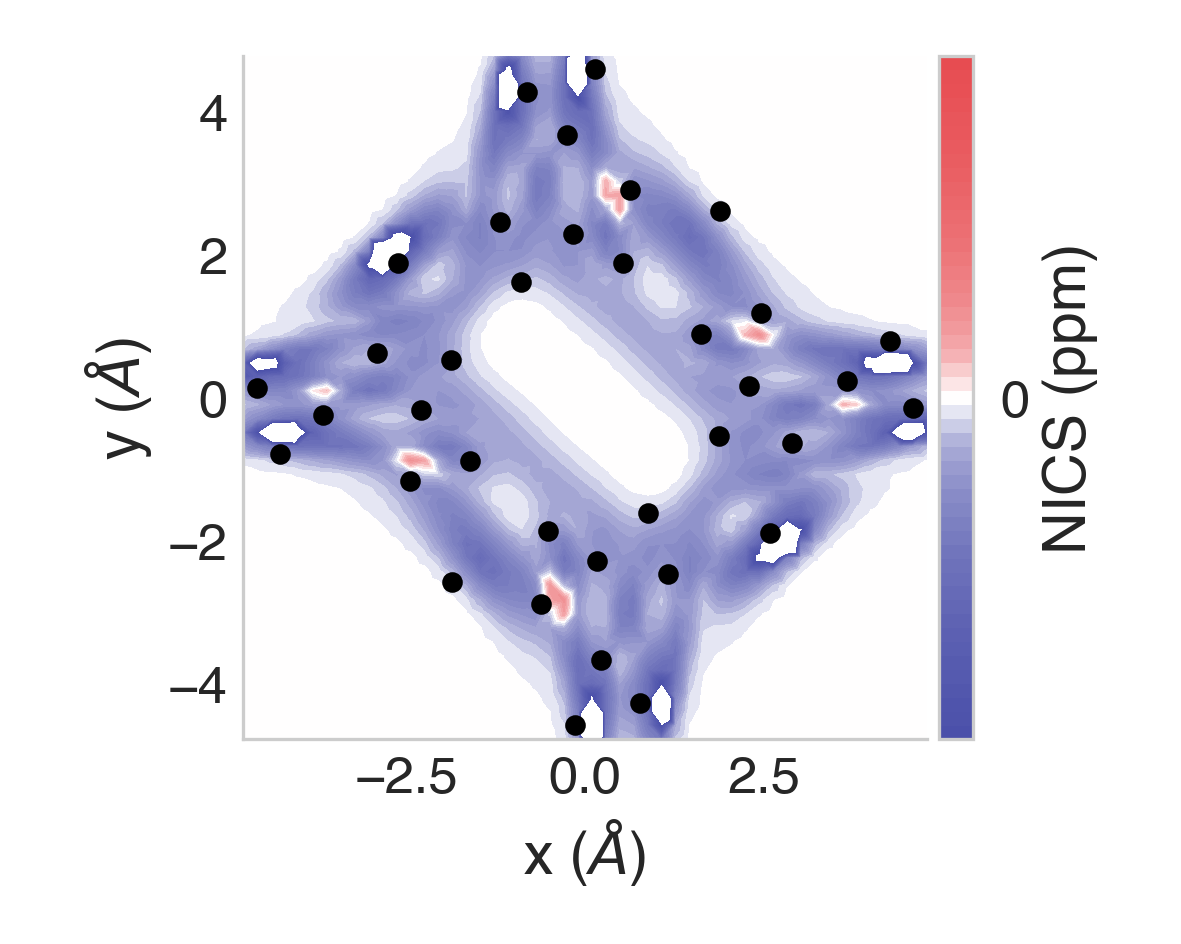
\includegraphics{se12-2d}\caption{NICS 2D projection for Se12.\\Aromatic character}\end{subfigure}
\begin{subfigure}{5.5cm}\centering\includegraphics{as08-2d}\caption{NICS 2D projection for As08.\\Antiaromatic character}\end{subfigure}%
\begin{subfigure}{5.5cm}\centering\includegraphics{as10-2d}\caption{NICS 2D projection for As10.\\Unclear but hints antiaromaticity}\end{subfigure}%
\begin{subfigure}{5.5cm}\centering\includegraphics{as12-2d}\caption{NICS 2D projection for As12.\\Unclear tendency, possibly antiaromatic}\end{subfigure}
\caption[Part 1 of NICS 2D projections]{Part 1 of NICS 2D projections}
\end{figure*}

\newpage

\begin{figure*}[h]
\centering
\begin{subfigure}{5.5cm}\centering\includegraphics{asn08-2d}\caption{NICS 2D projection for AsN08.\\Aromatic character}\end{subfigure}%
\begin{subfigure}{5.5cm}\centering\includegraphics{asn10-2d}\caption{NICS 2D projection for AsN10.\\Aromatic character}\end{subfigure}%
\begin{subfigure}{5.5cm}\centering\includegraphics{asn12-2d}\caption{NICS 2D projection for AsN12.\\Aromatic character}\end{subfigure}
\begin{subfigure}{5.5cm}\centering\includegraphics{p08-2d}\caption{NICS 2D projection for P08.\\Antiaromatic character}\end{subfigure}%
\begin{subfigure}{5.5cm}\centering\includegraphics{p10-2d}\caption{NICS 2D projection for P10.\\Antiaromatic character}\end{subfigure}%
\begin{subfigure}{5.5cm}\centering\includegraphics{p12-2d}\caption{NICS 2D projection for P12.\\Unclear tendency, possibly antiaromatic}\end{subfigure}
\begin{subfigure}{5.5cm}\centering\includegraphics{pn08-2d}\caption{NICS 2D projection for PN08.\\Aromatic character}\end{subfigure}%
\begin{subfigure}{5.5cm}\centering\includegraphics{pn10-2d}\caption{NICS 2D projection for PN10.\\Aromatic character}\end{subfigure}%
\begin{subfigure}{5.5cm}\centering\includegraphics{pn12-2d}\caption{NICS 2D projection for PN12.\\Aromatic character}\end{subfigure}
\caption[Part 2 of NICS 2D projections]{Part 2 of NICS 2D projections}
\end{figure*}


\newpage
\section{Raman spectra of all sunflowers}


\newpage
\section{UV-vis spectra of all sunflowers}
\labsec{ap:uv-vis-flowers}

As described in \refsec{uv-sunflowers}, \refsec{uv-stx} and \refsec{complex-uv}, UV-vis spectra was calculated and plotted for the lone sunflowers, the lone STX, and each of the flower-STX complexes.
The spectrum of each flower and spectrum the complex that it forms with STX have been displayed in the same graph for convenience and to allow for direct comparison.
The spectrum of lone STX has also been added as a reference.

\begin{figure*}[h]
\centering
\begin{subfigure}{8.25cm}\centering\includegraphics{uv-s08}\caption{UV-vis spectrum for S08}\end{subfigure}%
\begin{subfigure}{8.25cm}\centering\includegraphics{uv-se08}\caption{UV-vis spectrum for Se08}\end{subfigure}
\begin{subfigure}{8.25cm}\centering\includegraphics{uv-s10}\caption{UV-vis spectrum for S10}\end{subfigure}%
\begin{subfigure}{8.25cm}\centering\includegraphics{uv-se10}\caption{UV-vis spectrum for Se10}\end{subfigure}
\begin{subfigure}{8.25cm}\centering\includegraphics{uv-s12}\caption{UV-vis spectrum for S12}\end{subfigure}%
\begin{subfigure}{8.25cm}\centering\includegraphics{uv-se12}\caption{UV-vis spectrum for Se12}\end{subfigure}
\caption[Part 1 of flower UV-vis spectra]{Part 1 of flower UV-vis spectra}
\end{figure*}

\newpage

\begin{figure*}[h]
\centering
\begin{subfigure}{8.25cm}\centering\includegraphics{uv-as08}\caption{UV-vis spectrum for As08}\end{subfigure}%
\begin{subfigure}{8.25cm}\centering\includegraphics{uv-asn08}\caption{UV-vis spectrum for AsN08}\end{subfigure}
\begin{subfigure}{8.25cm}\centering\includegraphics{uv-as10}\caption{UV-vis spectrum for As10}\end{subfigure}%
\begin{subfigure}{8.25cm}\centering\includegraphics{uv-asn10}\caption{UV-vis spectrum for AsN10}\end{subfigure}
\begin{subfigure}{8.25cm}\centering\includegraphics{uv-as12}\caption{UV-vis spectrum for As12}\end{subfigure}%
\begin{subfigure}{8.25cm}\centering\includegraphics{uv-asn12}\caption{UV-vis spectrum for AsN12}\end{subfigure}
\caption[Part 2 of flower UV-vis spectra]{Part 2 of flower UV-vis spectra}
\end{figure*}

\newpage

\begin{figure*}[h]
\centering
\begin{subfigure}{8.25cm}\centering\includegraphics{uv-p08}\caption{UV-vis spectrum for P08}\end{subfigure}%
\begin{subfigure}{8.25cm}\centering\includegraphics{uv-pn08}\caption{UV-vis spectrum for PN08}\end{subfigure}
\begin{subfigure}{8.25cm}\centering\includegraphics{uv-p10}\caption{UV-vis spectrum for P10}\end{subfigure}%
\begin{subfigure}{8.25cm}\centering\includegraphics{uv-pn10}\caption{UV-vis spectrum for PN10}\end{subfigure}
\begin{subfigure}{8.25cm}\centering\includegraphics{uv-p12}\caption{UV-vis spectrum for P12}\end{subfigure}%
\begin{subfigure}{8.25cm}\centering\includegraphics{uv-pn12}\caption{UV-vis spectrum for PN12}\end{subfigure}
\caption[Part 3 of flower UV-vis spectra]{Part 3 of flower UV-vis spectra}
\end{figure*}


\newpage
\section{Combined enhancement factor graphs}
\labsec{ap:combined-ef}

\begin{figure*}[h]
\centering
\begin{subfigure}{8.25cm}\centering\includegraphics{comb-as10}\caption{Combined graph for As10-STX}\end{subfigure}%
\begin{subfigure}{8.25cm}\centering\includegraphics{comb-as12}\caption{Combined graph for As12-STX}\end{subfigure}
\begin{subfigure}{8.25cm}\centering\includegraphics{comb-asn08}\caption{Combined graph for AsN08-STX}\end{subfigure}%
\begin{subfigure}{8.25cm}\centering\includegraphics{comb-asn10}\caption{Combined graph for AsN10-STX}\end{subfigure}
\caption[Part 1 of combined EF RR graphs]{Part 1 of combined EF RR graphs}
\end{figure*}

\newpage

\begin{figure*}[h]
\centering
\begin{subfigure}{8.25cm}\centering\includegraphics{comb-asn12}\caption{Combined graph for AsN12-STX}\end{subfigure}%
\begin{subfigure}{8.25cm}\centering\includegraphics{comb-p12}\caption{Combined graph for P12-STX}\end{subfigure}
\begin{subfigure}{8.25cm}\centering\includegraphics{comb-pn10}\caption{Combined graph for PN10-STX}\end{subfigure}%
\begin{subfigure}{8.25cm}\centering\includegraphics{comb-pn12}\caption{Combined graph for PN12-STX}\end{subfigure}
\caption[Part 2 of combined EF RR graphs]{Part 2 of combined EF RR graphs}
\end{figure*}


\newpage
\section{Resonance Raman spectra}
\labsec{ap:rr}

\begin{figure*}[h]
    \includegraphics{unfolded-as10}
    \caption[RR spectra of As10-STX]{RR spectra of As10-STX. Selected $\lambda$: \SI{381}{\nano\metre}, \SI{432}{\nano\metre}, \SI{600}{\nano\metre}}
    \labfig{unfolded-as10}
\end{figure*}
\begin{figure*}[h]
    \includegraphics{unfolded-as12}
    \caption[RR spectra of As12-STX]{RR spectra of As12-STX. All of the lasers performed very similarly}
    \labfig{unfolded-as12}
\end{figure*}
\begin{figure*}[h]
    \includegraphics{unfolded-asn08}
    \caption[RR spectra of AsN08-STX]{RR spectra of AsN08-STX. Selected $\lambda$: \SI{384}{\nano\metre}, \SI{402}{\nano\metre}, \SI{498}{\nano\metre}}
    \labfig{unfolded-asn08}
\end{figure*}
\begin{figure*}[h]
    \includegraphics{unfolded-asn10}
    \caption[RR spectra of AsN10-STX]{RR spectra of AsN10-STX. All of the tested lasers resulted in similar amplifications}
    \labfig{unfolded-asn10}
\end{figure*}

\newpage

\begin{figure*}[h]
    \includegraphics{unfolded-asn12}
    \caption[RR spectra of AsN12-STX]{RR spectra of AsN12-STX. All of the lasers were considered equivalent in terms of amplifications, except for \SI{476}{\nano\metre}, which did not amplify mode 195}
    \labfig{unfolded-asn12}
\end{figure*}
\begin{figure*}[h]
    \includegraphics{unfolded-p12}
    \caption[RR spectra of P12-STX]{RR spectra of P12-STX. Selected $\lambda$: \SI{369}{\nano\metre}, \SI{447}{\nano\metre}}
    \labfig{unfolded-p12}
\end{figure*}
\begin{figure*}[h]
    \includegraphics{unfolded-pn10}
    \caption[RR spectra of PN10-STX]{RR spectra of PN10-STX. Selected $\lambda$: \SI{381}{\nano\metre}, \SI{525}{\nano\metre}}
    \labfig{unfolded-pn10}
\end{figure*}
\begin{figure*}[h]
    \includegraphics{unfolded-pn12}
    \caption[RR spectra of PN12-STX]{RR spectra of PN12-STX. All of the wavelengths were considered suitable}
    \labfig{unfolded-pn12}
\end{figure*}


\newpage
\section{Best Resonance Raman and derivatives}
\labsec{ap:rr-diff}

\begin{figure*}[h]
    \includegraphics{final-as10}
    \caption[RR spectra of As10-STX at \SI{381}{\nano\metre}]{RR spectra of As10-STX at \SI{381}{\nano\metre}}
    \labfig{final-as10}
\end{figure*}
\begin{figure*}[h]
    \includegraphics{final-as12}
    \caption[RR spectra of As12-STX at \SI{543}{\nano\metre}]{RR spectra of As12-STX at \SI{543}{\nano\metre}}
    \labfig{final-as12}
\end{figure*}
\begin{figure*}[h]
    \includegraphics{final-asn08}
    \caption[RR spectra of AsN08-STX at \SI{498}{\nano\metre}]{RR spectra of AsN08-STX at \SI{498}{\nano\metre}}
    \labfig{final-asn08}
\end{figure*}
\begin{figure*}[h]
    \includegraphics{final-asn10}
    \caption[RR spectra of AsN10-STX at \SI{618}{\nano\metre}]{RR spectra of AsN10-STX at \SI{618}{\nano\metre}}
    \labfig{final-asn10}
\end{figure*}

\newpage

\begin{figure*}[h]
    \includegraphics{final-asn12}
    \caption[RR spectra of AsN12-STX at \SI{707}{\nano\metre}]{RR spectra of AsN12-STX at \SI{707}{\nano\metre}}
    \labfig{final-asn12}
\end{figure*}
\begin{figure*}[h]
    \includegraphics{final-p12}
    \caption[RR spectra of P12-STX at \SI{447}{\nano\metre}]{RR spectra of P12-STX at \SI{447}{\nano\metre}}
    \labfig{final-p12}
\end{figure*}
\begin{figure*}[h]
    \includegraphics{final-pn10}
    \caption[RR spectra of PN10-STX at \SI{525}{\nano\metre}]{RR spectra of PN10-STX at \SI{525}{\nano\metre}}
    \labfig{final-pn10}
\end{figure*}
\begin{figure*}[h]
    \includegraphics{final-pn12}
    \caption[RR spectra of PN12-STX at \SI{616}{\nano\metre}]{RR spectra of PN12-STX at \SI{616}{\nano\metre}}
    \labfig{final-pn12}
\end{figure*}

\pagelayout{margin}

%----------------------------------------------------------------------------------------

\backmatter % Denotes the end of the main document content
\setchapterstyle{plain} % Output plain chapters from this point onwards

%----------------------------------------------------------------------------------------
%	BIBLIOGRAPHY
%----------------------------------------------------------------------------------------

% The bibliography needs to be compiled with biber using your LaTeX editor, or on the command line with 'biber main' from the template directory

\defbibnote{bibnote}{} % Prepend this text to the bibliography
\printbibliography[heading=bibintoc, title=Bibliography, prenote=bibnote] % Add the bibliography heading to the ToC, set the title of the bibliography and output the bibliography note

%----------------------------------------------------------------------------------------
%	GREEK ALPHABET
% 	Originally from https://gitlab.com/jim.hefferon/linear-algebra
%----------------------------------------------------------------------------------------
%
%\vspace{1cm}
%
%{\usekomafont{chapter}Greek Letters with Pronounciation} \\[2ex]
%\begin{center}
%	\newcommand{\pronounced}[1]{\hspace*{.2em}\small\textit{#1}}
%	\begin{tabular}{l l @{\hspace*{3em}} l l}
%		\toprule
%		Character & Name & Character & Name \\
%		\midrule
%		$\alpha$ & alpha \pronounced{AL-fuh} & $\nu$ & nu \pronounced{NEW} \\
%		$\beta$ & beta \pronounced{BAY-tuh} & $\xi$, $\Xi$ & xi \pronounced{KSIGH} \\
%		$\gamma$, $\Gamma$ & gamma \pronounced{GAM-muh} & o & omicron \pronounced{OM-uh-CRON} \\
%		$\delta$, $\Delta$ & delta \pronounced{DEL-tuh} & $\pi$, $\Pi$ & pi \pronounced{PIE} \\
%		$\epsilon$ & epsilon \pronounced{EP-suh-lon} & $\rho$ & rho \pronounced{ROW} \\
%		$\zeta$ & zeta \pronounced{ZAY-tuh} & $\sigma$, $\Sigma$ & sigma \pronounced{SIG-muh} \\
%		$\eta$ & eta \pronounced{AY-tuh} & $\tau$ & tau \pronounced{TOW (as in cow)} \\
%		$\theta$, $\Theta$ & theta \pronounced{THAY-tuh} & $\upsilon$, $\Upsilon$ & upsilon \pronounced{OOP-suh-LON} \\
%		$\iota$ & iota \pronounced{eye-OH-tuh} & $\phi$, $\Phi$ & phi \pronounced{FEE, or FI (as in hi)} \\
%		$\kappa$ & kappa \pronounced{KAP-uh} & $\chi$ & chi \pronounced{KI (as in hi)} \\
%		$\lambda$, $\Lambda$ & lambda \pronounced{LAM-duh} & $\psi$, $\Psi$ & psi \pronounced{SIGH, or PSIGH} \\
%		$\mu$ & mu \pronounced{MEW} & $\omega$, $\Omega$ & omega \pronounced{oh-MAY-guh} \\
%		\bottomrule
%	\end{tabular} \\[1.5ex]
%	Capitals shown are the ones that differ from Roman capitals.
%\end{center}
%
%----------------------------------------------------------------------------------------
%	GLOSSARY
%----------------------------------------------------------------------------------------

% The glossary needs to be compiled on the command line with 'makeglossaries main' from the template directory

\newglossaryentry{computer}{
	name=computer,
	description={is a programmable machine that receives input, stores and manipulates data, and provides output in a useful format}
}

% Glossary entries (used in text with e.g. \acrfull{fpsLabel} or \acrshort{fpsLabel})
\newacronym[longplural={Frames per Second}]{fpsLabel}{FPS}{Frame per Second}
\newacronym[longplural={Tables of Contents}]{tocLabel}{TOC}{Table of Contents}

\setglossarystyle{listgroup} % Set the style of the glossary (see https://en.wikibooks.org/wiki/LaTeX/Glossary for a reference)
\printglossary[title=Special Terms, toctitle=List of Terms] % Output the glossary, 'title' is the chapter heading for the glossary, toctitle is the table of contents heading

%----------------------------------------------------------------------------------------
%	INDEX
%----------------------------------------------------------------------------------------

% The index needs to be compiled on the command line with 'makeindex main' from the template directory

\printindex % Output the index

%----------------------------------------------------------------------------------------
%	BACK COVER
%----------------------------------------------------------------------------------------

% If you have a PDF/image file that you want to use as a back cover, uncomment the following lines

%\clearpage
%\thispagestyle{empty}
%\null%
%\clearpage
%\includepdf{cover-back.pdf}

%----------------------------------------------------------------------------------------

\end{document}
